% ============================================================
% Avance 7: Resumen Ejecutivo — EpiForecast-MX
% Equipo 01 | MNA | Tec de Monterrey
% Marzo 2026
% ============================================================
\documentclass[12pt, letterpaper]{article}

% --- Codificación y fuentes ---
\usepackage[utf8]{inputenc}
\usepackage[T1]{fontenc}
\usepackage{lmodern}
\usepackage[spanish, es-tabla]{babel}

% --- Micro-tipografia ---
\IfFileExists{microtype.sty}{\usepackage[tracking=true, kerning=true, spacing=true]{microtype}}{}

% --- Geometria ---
\usepackage[letterpaper, margin=2.5cm, top=3cm, bottom=2.5cm]{geometry}
\setlength{\headheight}{14pt}
\setlength{\emergencystretch}{3em}

% --- Gráficos y figuras ---
\usepackage{graphicx}
\graphicspath{{../FigResumenEjecutivo/}{FigResumenEjecutivo/}{FigurasConclu/}{FigurasTableau/}}
\usepackage{float}
\usepackage{subcaption}

% --- Tablas ---
\usepackage{booktabs}
\usepackage{tabularx}
\usepackage{longtable}
\usepackage{array}

% --- Colores ---
\usepackage{xcolor}
\usepackage{colortbl}

% Paleta institucional IMSS
\definecolor{burgundy}{HTML}{9B2242}
\definecolor{darkburgundy}{HTML}{6F1D46}
\definecolor{teal}{HTML}{00524E}
\definecolor{lightteal}{HTML}{3D8B84}
\definecolor{darkteal}{HTML}{173F35}
\definecolor{gold}{HTML}{B58500}
\definecolor{coolgray}{HTML}{97999B}
\definecolor{imssblue}{HTML}{003A70}
\definecolor{cream}{HTML}{F5EDE0}
\definecolor{lightgreen}{HTML}{E6F4EA}
\definecolor{lightyellow}{HTML}{FEF7E0}
\definecolor{lightred}{HTML}{FDE8E8}

% Colores por motor de pronóstico
\definecolor{cprophet}{HTML}{004D40}
\definecolor{cdeepar}{HTML}{880E4F}
\definecolor{censemble}{HTML}{FF6F00}
\definecolor{cstacking}{HTML}{1A237E}

% --- Encabezados y pies ---
\usepackage{fancyhdr}
\pagestyle{fancy}
\fancyhf{}
\fancyhead[L]{\small\textcolor{coolgray}{EpiForecast-MX | Avance~7: Resumen Ejecutivo}}
\fancyhead[R]{\small\textcolor{coolgray}{Equipo 01 | MNA | Tec de Monterrey}}
\fancyfoot[C]{\thepage}
\fancyfoot[R]{\small\textcolor{coolgray}{Marzo 2026}}
\renewcommand{\headrulewidth}{0.4pt}
\renewcommand{\footrulewidth}{0.2pt}

% --- Titulos de sección (requiere titlesec en Overleaf) ---
\IfFileExists{titlesec.sty}{%
  \usepackage{titlesec}
  \titleformat{\section}
    {\Large\bfseries\color{teal}}{\thesection.}{0.5em}{}[\vspace{-0.5em}\textcolor{teal}{\rule{\textwidth}{1pt}}]
  \titleformat{\subsection}
    {\large\bfseries\color{burgundy}}{\thesubsection}{0.5em}{}
  \titleformat{\subsubsection}
    {\normalsize\bfseries\color{darkteal}}{\thesubsubsection}{0.5em}{}
}{}

% --- Listas ---
\IfFileExists{enumitem.sty}{\usepackage{enumitem}}{}

% --- Matematicas ---
\usepackage{amsmath, amssymb}

% --- Captions ---
\usepackage{caption}
\captionsetup{
    font={small, color=coolgray},
    labelfont={bf, color=coolgray},
    justification=centering
}

% --- Cajas destacadas ---
% Usa tcolorbox si está disponible (Overleaf), sino usa fallback simple
\newif\ifhavetcolorbox
\IfFileExists{tcolorbox.sty}{\havetcolorboxtrue}{\havetcolorboxfalse}

\ifhavetcolorbox
  \usepackage[most]{tcolorbox}
  \newtcolorbox{insightbox}[1][]{
    colback=lightgreen, colframe=teal,
    left=8pt, right=8pt, top=6pt, bottom=6pt,
    boxrule=0pt, leftrule=4pt, arc=0pt,
    before upper={\setlength{\emergencystretch}{5em}}, #1
  }
  \newtcolorbox{warningbox}[1][]{
    colback=lightyellow, colframe=gold,
    left=8pt, right=8pt, top=6pt, bottom=6pt,
    boxrule=0pt, leftrule=4pt, arc=0pt,
    before upper={\setlength{\emergencystretch}{5em}}, #1
  }
  \newtcolorbox{criticalbox}[1][]{
    colback=lightred, colframe=burgundy,
    left=8pt, right=8pt, top=6pt, bottom=6pt,
    boxrule=0pt, leftrule=4pt, arc=0pt,
    before upper={\setlength{\emergencystretch}{5em}}, #1
  }
  \newtcolorbox{kpibox}[1][]{
    colback=white, colframe=gold, boxrule=2pt, arc=6pt,
    left=12pt, right=12pt, top=8pt, bottom=8pt,
    before upper={\setlength{\emergencystretch}{5em}}, #1
  }
\else
  % Fallback: cajas simples con colorbox
  \newsavebox{\boxcontents}
  \newenvironment{insightbox}[1][]{\par\medskip\begin{lrbox}{\boxcontents}\begin{minipage}{\dimexpr\textwidth-12pt}\setlength{\emergencystretch}{5em}\setlength{\parskip}{6pt}}{\end{minipage}\end{lrbox}\noindent\colorbox{lightgreen}{\usebox{\boxcontents}}\par\medskip}
  \newenvironment{warningbox}[1][]{\par\medskip\begin{lrbox}{\boxcontents}\begin{minipage}{\dimexpr\textwidth-12pt}\setlength{\emergencystretch}{5em}\setlength{\parskip}{6pt}}{\end{minipage}\end{lrbox}\noindent\colorbox{lightyellow}{\usebox{\boxcontents}}\par\medskip}
  \newenvironment{criticalbox}[1][]{\par\medskip\begin{lrbox}{\boxcontents}\begin{minipage}{\dimexpr\textwidth-12pt}\setlength{\emergencystretch}{5em}\setlength{\parskip}{6pt}}{\end{minipage}\end{lrbox}\noindent\colorbox{lightred}{\usebox{\boxcontents}}\par\medskip}
  \newenvironment{kpibox}[1][]{\par\medskip\begin{lrbox}{\boxcontents}\begin{minipage}{\dimexpr\textwidth-12pt}\setlength{\emergencystretch}{5em}\setlength{\parskip}{6pt}}{\end{minipage}\end{lrbox}\noindent\fbox{\usebox{\boxcontents}}\par\medskip}
\fi

% --- Iconos ---
\usepackage{pifont}
\IfFileExists{fontawesome5.sty}{\usepackage{fontawesome5}}{}

% --- Espaciado ---
\usepackage{parskip}
\usepackage{setspace}

% --- Pie de página ---
\IfFileExists{footmisc.sty}{\usepackage[bottom]{footmisc}}{}

% --- URLs ---
\IfFileExists{xurl.sty}{\usepackage{xurl}}{}

% --- Hyperlinks ---
\usepackage[breaklinks=true]{hyperref}
\hypersetup{
    colorlinks=true,
    linkcolor=teal,
    citecolor=burgundy,
    urlcolor=imssblue,
    bookmarksopen=true,
    pdftitle={EpiForecast-MX | Avance~7: Resumen Ejecutivo},
    pdfauthor={Equipo 01 | MNA Tec de Monterrey},
}

% --- TikZ ---
\usepackage{tikz}
\usetikzlibrary{arrows.meta, positioning, shapes.geometric, fit, calc, decorations.pathreplacing, babel}

% --- Landscape ---
\usepackage{pdflscape}

% --- Multicol ---
\usepackage{multicol}

% --- Bibliografia ---
% Nota: las referencias se manejan manualmente en formato APA 7
% (mismo estilo que Avance~6). El archivo references_avance7.bib
% está disponible para compilación con biblatex en Overleaf si se prefiere.

% --- Comandos personalizados ---
\newcommand{\smape}{\textnormal{\textsc{smape}}}
\newcommand{\mase}{\textnormal{\textsc{mase}}}
\newcommand{\rmse}{\textnormal{\textsc{rmse}}}
\newcommand{\mae}{\textnormal{\textsc{mae}}}
\newcommand{\mape}{\textnormal{\textsc{mape}}}
\newcommand{\imss}{\textnormal{\textsc{imss}}}
% Badges de riesgo con color
\newcommand{\riskHigh}{\cellcolor{lightred}\textbf{\textcolor{burgundy}{Alta}}}
\newcommand{\riskMed}{\cellcolor{lightyellow}\textbf{\textcolor{gold}{Media}}}
\newcommand{\riskLow}{\cellcolor{lightgreen}\textbf{\textcolor{darkteal}{Baja}}}
\newcommand{\tabref}[1]{Tabla~\ref{#1}}
\newcommand{\figref}[1]{Figura~\ref{#1}}
\newcommand{\secref}[1]{Sección~\ref{#1}}
\newcommand{\sepsection}{\vspace{0.5cm}\noindent\textcolor{coolgray}{\rule{\textwidth}{0.3pt}}\vspace{0.3cm}}

% ============================================================
\begin{document}
\shorthandoff{<>}

% ============================================================
% PORTADA
% ============================================================
\thispagestyle{empty}
% --- Fondo TikZ de la portada ---
\begin{tikzpicture}[remember picture, overlay]
  % Franja superior blanca para logos (1.8cm)
  \fill[white] (current page.north west) rectangle ([yshift=-1.8cm]current page.north east);
  % Linea gold de transicion entre zona blanca y burgundy
  \fill[gold] ([yshift=-1.8cm]current page.north west) rectangle ([yshift=-1.95cm]current page.north east);
  % Bloque burgundy con degradado (9cm)
  \shade[top color=burgundy, bottom color=darkburgundy]
    ([yshift=-1.95cm]current page.north west) rectangle ([yshift=-11.5cm]current page.north east);
  % Patron de puntos decorativo (watermark sutil)
  \foreach \x in {-8,-7,...,8} {
    \foreach \y in {0,1,...,5} {
      \fill[white, opacity=0.03] ([yshift=-2.5cm-\y*1.5cm, xshift=\x*2.2cm]current page.north) circle (0.8pt);
    }
  }
  % Franja teal (0.8cm)
  \fill[teal] ([yshift=-11.5cm]current page.north west) rectangle ([yshift=-12.3cm]current page.north east);
  % Franja gold (0.4cm)
  \fill[gold] ([yshift=-12.3cm]current page.north west) rectangle ([yshift=-12.7cm]current page.north east);
  % Franja inferior burgundy
  \fill[burgundy] ([yshift=1.2cm]current page.south west) rectangle (current page.south east);
\end{tikzpicture}

% --- Logos institucionales ---
\vspace*{-1.0cm}
\noindent
\begin{minipage}{0.3\textwidth}
\raggedright
\setlength{\fboxsep}{4pt}\setlength{\fboxrule}{0pt}%
\fcolorbox{white}{white}{
\includegraphics[height=1.2cm]{logo_imss.png}}
\end{minipage}%
\hfill
\begin{minipage}{0.3\textwidth}
\raggedleft
\setlength{\fboxsep}{4pt}\setlength{\fboxrule}{0pt}%
\fcolorbox{white}{white}{
\includegraphics[height=1.2cm]{logo_tec.png}}
\end{minipage}

% --- Titulo principal (dentro del bloque burgundy) ---
\vspace{1.0cm}

\begin{center}
{\color{white}\fontsize{12}{16}\selectfont\textsc{Instituto Mexicano del Seguro Social $\bullet$ Tecnológico de Monterrey}}\\[0.2cm]
{\color{white!70}\fontsize{10}{14}\selectfont Maestría en Inteligencia Artificial Aplicada | Proyecto Integrador | Equipo 01}\\[1.2cm]
{\color{white}\fontsize{30}{36}\selectfont\bfseries E\kern0.5pt p\kern0.5pt i\kern0.5pt F\kern0.5pt o\kern0.5pt r\kern0.5pt e\kern0.5pt c\kern0.5pt a\kern0.5pt s\kern0.5pt t\kern0.5pt -\kern0.5pt M\kern0.5pt X}\\[0.5cm]
{\color{gold}\fontsize{14}{20}\selectfont\bfseries\itshape Generalización de modelos nacionales de pronóstico\\
epidemiológico hacia un enfoque modular con desagregación\\
por sexo y entidad federativa en México}\\[1.0cm]
\end{center}

% --- Avance~7 (debajo de franjas) ---
\vspace{1.3cm}

\begin{center}
{\color{teal}\fontsize{20}{26}\selectfont\bfseries AVANCE 7: RESUMEN EJECUTIVO}\\[1.0cm]
\end{center}

% --- Mini-KPIs en portada ---
\begin{center}
\setlength{\tabcolsep}{8pt}
\begin{tabular}{cccc}
\textcolor{burgundy}{\fontsize{22}{26}\selectfont\bfseries 333} &
\textcolor{burgundy}{\fontsize{22}{26}\selectfont\bfseries 94.9\%} &
\textcolor{burgundy}{\fontsize{22}{26}\selectfont\bfseries 52} &
\textcolor{burgundy}{\fontsize{22}{26}\selectfont\bfseries 506} \\
{\scriptsize modelos en} & {\scriptsize superan la línea} & {\scriptsize semanas de} & {\scriptsize USD costo} \\
{\scriptsize producción} & {\scriptsize base naive} & {\scriptsize horizonte} & {\scriptsize operativo anual} \\
\end{tabular}
\end{center}

\vspace{2.5cm}

% --- Bloque de autores ---
\begin{center}
\small
\begin{tabular}{ll}
\textcolor{burgundy}{\bfseries Autores:} & Javier A. Rebull Saucedo \textcolor{coolgray}{(A01795838)} \\
 & Juan Carlos Perez Nava \textcolor{coolgray}{(A01795941)} \\
 & Luis G. Sanchez Salazar \textcolor{coolgray}{(A01232963)} \\[0.3cm]
\textcolor{burgundy}{\bfseries Asesora:} & Dra.~Grettel Barcelo Alonso \\[0.15cm]
\textcolor{burgundy}{\bfseries Expertas IMSS:} & Dra.~Ruth Perez-Hernandez | Dra.~Lina Diaz Castro \\[0.3cm]
\textcolor{burgundy}{\bfseries Fecha:} & Marzo 2026 \\
\end{tabular}
\end{center}

\vspace{0.3cm}

% --- URL en franja inferior ---
\begin{tikzpicture}[remember picture, overlay]
  \node[anchor=south, yshift=0.3cm] at (current page.south) {%
    \color{white}\normalsize\texttt{proyectointegrador.org} \quad
    {\color{gold}\small|}  \quad
    {\color{white!80}\small EpiForecast-MX \textbar{} Equipo 01}%
  };
\end{tikzpicture}

\newpage

% ============================================================
% INDICES
% ============================================================
\tableofcontents
\newpage
\listoffigures
\listoftables
\newpage

% ============================================================
% PAGINA KPIs "AT A GLANCE"
% ============================================================
\thispagestyle{empty}
\vspace*{1cm}
\begin{center}
{\color{teal}\fontsize{22}{28}\selectfont\bfseries EpiForecast-MX en Números}\\[0.3cm]
{\color{coolgray}\normalsize Indicadores clave del sistema de pronóstico epidemiológico}
\end{center}

\vspace{1.0cm}

\begin{center}
\setlength{\fboxsep}{15pt}

% Fila 1: tres KPIs
\noindent
\begin{minipage}[t]{0.31\textwidth}
\centering
\colorbox{lightred}{%
\begin{minipage}[c][3.5cm]{\dimexpr\textwidth-30pt}
\centering
{\color{burgundy}\fontsize{36}{40}\selectfont\bfseries 333}\\[0.3cm]
{\small\bfseries Modelos en Producción}\\[0.15cm]
{\scriptsize\color{coolgray} 37~geografías $\times$ 3~condiciones $\times$ 3~segmentos}
\end{minipage}}
\end{minipage}\hfill
\begin{minipage}[t]{0.31\textwidth}
\centering
\colorbox{lightgreen}{%
\begin{minipage}[c][3.5cm]{\dimexpr\textwidth-30pt}
\centering
{\color{teal}\fontsize{36}{40}\selectfont\bfseries 94.9\%}\\[0.3cm]
{\small\bfseries Superan Línea Base}\\[0.15cm]
{\scriptsize\color{coolgray} \smape{} mediana: 23.66\% | \mase{}: 0.30}
\end{minipage}}
\end{minipage}\hfill
\begin{minipage}[t]{0.31\textwidth}
\centering
\colorbox{lightyellow}{%
\begin{minipage}[c][3.5cm]{\dimexpr\textwidth-30pt}
\centering
{\color{gold}\fontsize{36}{40}\selectfont\bfseries 52}\\[0.3cm]
{\small\bfseries Semanas de Horizonte}\\[0.15cm]
{\scriptsize\color{coolgray} Cobertura nacional, 32~entidades}
\end{minipage}}
\end{minipage}

\vspace{0.8cm}

% Fila 2: tres KPIs
\noindent
\begin{minipage}[t]{0.31\textwidth}
\centering
\colorbox{lightyellow}{%
\begin{minipage}[c][3.5cm]{\dimexpr\textwidth-30pt}
\centering
{\color{gold}\fontsize{30}{36}\selectfont\bfseries 165,449}\\[0.3cm]
{\small\bfseries Casos Pronosticados/Año}\\[0.15cm]
{\scriptsize\color{coolgray} Depresión, Parkinson, Alzheimer (Nacional)}
\end{minipage}}
\end{minipage}\hfill
\begin{minipage}[t]{0.31\textwidth}
\centering
\colorbox{lightgreen}{%
\begin{minipage}[c][3.5cm]{\dimexpr\textwidth-30pt}
\centering
{\color{teal}\fontsize{30}{36}\selectfont\bfseries \$240\,--\,\$506}\\[0.3cm]
{\small\bfseries USD Costo Anual}\\[0.15cm]
{\scriptsize\color{coolgray} Equivale a 4~consultas de especialidad}
\end{minipage}}
\end{minipage}\hfill
\begin{minipage}[t]{0.31\textwidth}
\centering
\colorbox{lightred}{%
\begin{minipage}[c][3.5cm]{\dimexpr\textwidth-30pt}
\centering
{\color{burgundy}\fontsize{36}{40}\selectfont\bfseries 92\%}\\[0.3cm]
{\small\bfseries Ahorro GPU}\\[0.15cm]
{\scriptsize\color{coolgray} Reentrenamiento trimestral vs.~semanal}
\end{minipage}}
\end{minipage}

\end{center}

\vspace{1.0cm}

% Barra de motores
\begin{center}
{\color{coolgray}\small Distribución de motores ganadores en las 333~series de producción}\\[0.3cm]
\begin{tikzpicture}
  % Barra de proporción
  \fill[cdeepar] (0,0) rectangle (0.733*14,0.7);
  \fill[cprophet] (0.733*14,0) rectangle ({(0.733+0.165)*14},0.7);
  \fill[censemble] ({(0.733+0.165)*14},0) rectangle ({(0.733+0.165+0.096)*14},0.7);
  \fill[cstacking] ({(0.733+0.165+0.096)*14},0) rectangle (14,0.7);
  % Labels
  \node[white, font=\small\bfseries] at (0.733*7, 0.35) {DeepAR 73.3\%};
  \node[white, font=\tiny\bfseries] at ({(0.733+0.165/2)*14}, 0.35) {Prophet};
  \node[white, font=\tiny] at ({(0.733+0.165+0.096/2)*14}, 0.35) {Ens.};
\end{tikzpicture}\\[0.2cm]
{\scriptsize\color{coolgray}
\textcolor{cdeepar}{\rule{8pt}{8pt}}~DeepAR 73.3\% (244) \quad
\textcolor{cprophet}{\rule{8pt}{8pt}}~Prophet 16.5\% (55) \quad
\textcolor{censemble}{\rule{8pt}{8pt}}~Ensemble 9.6\% (32) \quad
\textcolor{cstacking}{\rule{8pt}{8pt}}~Stacking 0.6\% (2)}
\end{center}

\newpage

% ============================================================
% ABSTRACT
% ============================================================
\section*{Abstract}\label{sec:abstract}
\addcontentsline{toc}{section}{Abstract}

EpiForecast-MX es una plataforma de inteligencia epidemiológica desarrollada en colaboración con el Instituto Mexicano del Seguro Social (\imss{}) para pronosticar la incidencia semanal de tres condiciones neurológicas y de salud mental: Depresión (F32), Parkinson (G20) y Alzheimer (G30). El sistema abarca las 32~entidades federativas de México, desagregado por sexo, con un horizonte de predicción de 52~semanas.

La arquitectura multi-motor evalúa cuatro algoritmos de aprendizaje automático (DeepAR, Prophet, Ensemble (Prophet + XGBoost) y Stacking (Prophet + ETS + LightGBM + Ridge)) sobre 1,332 combinaciones, seleccionando automáticamente el mejor modelo para cada una de las 333~series de producción. DeepAR domina con el 73.3\% de las selecciones, seguido por Prophet (16.5\%), Ensemble (9.6\%) y Stacking (0.6\%). El sistema alcanza una mediana global de \smape{} de 23.66\% y un \mase{} de 0.30, superando la línea base naive en el 94.9\% de las series.

La plataforma opera sobre infraestructura MLOps completa (AWS SageMaker, DVC, GitHub Actions) con un costo operativo anual proyectado de 240--506~USD. El ecosistema incluye un dashboard interactivo Tableau para tomadores de decisiones, una consola CLI para el equipo técnico y un asistente conversacional web para médicos y público general. Este documento sintetiza los hallazgos de siete avances de desarrollo, presenta un análisis costo--beneficio por fase CRISP-ML(Q) y mapea los riesgos asociados al despliegue de modelos de aprendizaje automático en el sector salud.

\vspace{0.5cm}
\noindent\textbf{\textcolor{burgundy}{Palabras clave:}} pronóstico epidemiológico, aprendizaje automático, series de tiempo, IMSS, DeepAR, Prophet, CRISP-ML(Q), salud pública, México, MLOps.

\sepsection

% ============================================================
% PAGINA DE CITA
% ============================================================
\newpage
\thispagestyle{empty}
\vspace*{\fill}
\begin{center}
\begin{minipage}{0.85\textwidth}
\begin{center}
{\color{burgundy}\fontsize{70}{70}\selectfont\textbf{``}}\\[0.5cm]
{\color{darkteal}\fontsize{18}{26}\selectfont\itshape
Si la causa latente de las epidemias no puede descubrirse, el modo en que opera puede investigarse. Las leyes de su acción pueden determinarse por observación, así como las circunstancias en que las epidemias surgen o por las cuales pueden ser controladas.}\\[0.8cm]
{\color{coolgray}\normalsize --- William Farr, 1840}
\end{center}
\end{minipage}
\end{center}
\vspace*{\fill}
\newpage

% ============================================================
% 1. INTRODUCCION
% ============================================================
\section{Introducción}\label{sec:introduccion}

Pronosticar el clima a siete días cuesta miles de millones de dólares en supercomputadoras. Pronosticar la demanda de atención en salud mental para 80~millones de mexicanos, con 52~semanas de anticipación y cobertura en las 32~entidades federativas, cuesta menos que cuatro consultas de neurología al año. Esa es la promesa, y la realidad operativa, de EpiForecast-MX.

Para el \imss{}, anticipar la demanda de atención médica no es un ejercicio académico: es la diferencia entre tener suficientes consultorios de psiquiatría en Jalisco la próxima primavera o dejar a cientos de pacientes con depresión en lista de espera; entre distribuir medicamento antiparkinsoniano a tiempo en Nuevo León o enfrentar desabastos que afectan la calidad de vida de miles de personas.

Hasta ahora, el \imss{} ha operado de manera \textbf{reactiva} frente a las enfermedades neurológicas y de salud mental. Los datos del Sistema Nacional de Vigilancia Epidemiológica (SINAVE) se recopilan semanalmente, pero su uso se limita a reportes descriptivos del pasado. No existe un sistema institucional que transforme esos datos en \textbf{pronósticos accionables} a mediano plazo.

EpiForecast-MX nace para cerrar esa brecha. Es la primera plataforma de pronóstico epidemiológico multi-modelo del \imss{} que predice, con un horizonte de 52~semanas, la incidencia semanal de tres condiciones del sistema nervioso clasificadas en la CIE-10:

\begin{itemize}
  \item \textbf{Depresión (F32):} el padecimiento con mayor volumen (más de 155,000~casos pronosticados al año a nivel nacional), con un diferencial de género marcado donde las mujeres representan aproximadamente el 70\% de los casos.
  \item \textbf{Parkinson (G20):} la segunda enfermedad neurodegenerativa más común a nivel mundial, con impacto creciente por el envejecimiento poblacional en México.
  \item \textbf{Alzheimer (G30):} condición de baja incidencia registrada pero con enorme carga económica y social, donde el subregistro es un desafío conocido.
\end{itemize}

El proyecto fue desarrollado por un equipo interdisciplinario de la Maestría en Inteligencia Artificial Aplicada (MNA) del Tecnológico de Monterrey, en colaboración directa con investigadoras del \imss{}, la Dra.~Ruth Perez-Hernandez y la Dra.~Lina Diaz Castro, quienes aportaron la visión clínica y el contexto institucional indispensable para que los modelos tengan relevancia práctica.

Este resumen ejecutivo sintetiza siete meses de trabajo intensivo, desde la comprensión del problema hasta la propuesta de despliegue en producción, con el objetivo de presentar a los tomadores de decisiones del \imss{} una visión clara del \textbf{valor entregado}, los \textbf{costos asociados} y los \textbf{riesgos a considerar}.

% ============================================================
% 2. SINTESIS DEL PROBLEMA
% ============================================================
\newpage
\section{Síntesis del problema}\label{sec:problema}

\subsection{El contexto epidemiológico}

Las enfermedades neurológicas representan la principal causa de discapacidad a nivel mundial (IHME, 2021). En México, la transición demográfica, con una población que envejece rápidamente, intensifica la presión sobre los servicios de neurología y psiquiatría del \imss{}, que atiende a más del 50\% de la población asegurada del país (IMSS, 2024).

La Organización Mundial de la Salud estima que más de 8.5~millones de personas viven con Parkinson globalmente, cifra que se ha duplicado en los últimos 25~años; la discapacidad y mortalidad por esta enfermedad crecen más rápido que las de cualquier otro trastorno neurológico (OMS, 2022). Para Alzheimer, se estiman entre 1.3 y 1.8~millones de personas afectadas en México, con un costo anual que supera los 115,000~millones de pesos por familia (ADI, 2015). La depresión afecta a entre 8 y 10~millones de mexicanos, y la OMS ha demostrado que cada dólar invertido en tratamiento de depresión y ansiedad genera un retorno de 4~dólares en salud y productividad (OMS, 2016).

\subsection{La brecha operativa}

El \imss{} recopila datos epidemiológicos semanales a través del SINAVE desde 2014, generando un acervo histórico de más de una década. Sin embargo, estos datos se han utilizado principalmente de forma \textbf{descriptiva}: reportes sobre lo que \emph{ya ocurrió}, no sobre lo que \emph{está por ocurrir}. Las limitaciones identificadas al inicio del proyecto incluyen:

\begin{enumerate}
  \item \textbf{Ausencia de capacidad predictiva:} no existía un sistema que generara pronósticos de incidencia a mediano o largo plazo para estas tres condiciones.
  \item \textbf{Datos en formato PDF:} los boletines SINAVE se publican como documentos PDF, requiriendo un pipeline de extracción automatizada.
  \item \textbf{Complejidad geográfica:} 32~entidades federativas con patrones epidemiológicos heterogéneos, donde un modelo único no puede capturar todas las dinámicas locales.
  \item \textbf{Anomalías COVID-19:} el periodo 2020--2022 introdujo disrupciones severas en los patrones de reporte epidemiológico, exigiendo estrategias específicas de tratamiento de datos.
\end{enumerate}

\subsection{El impacto potencial}

Un sistema de pronóstico confiable permite al \imss{}:

\begin{insightbox}
\textbf{Planificación de recursos:} distribuir consultorios, especialistas y turnos de atención basándose en la demanda proyectada, no en la inercia histórica.\\[0.3cm]
\textbf{Gestión farmacológica:} anticipar la demanda de medicamentos antiparkinsonianos, antidepresivos e inhibidores de colinesterasa para evitar desabastos y reducir desperdicios.\\[0.3cm]
\textbf{Equidad en atención:} identificar disparidades por género y región, asegurando que la distribución de recursos refleje las necesidades reales de cada entidad.\\[0.3cm]
\textbf{Política pública basada en evidencia:} proporcionar a la Secretaría de Salud proyecciones que sustenten decisiones presupuestales y programas de prevención.
\end{insightbox}

% ============================================================
% 3. HALLAZGOS CLAVE DEL EDA
% ============================================================
\newpage
\section{Hallazgos clave del análisis exploratorio}\label{sec:eda}

El análisis exploratorio de datos (EDA), presentado en detalle en el Avance~1 (Rebull et al., 2026a), reveló patrones epidemiológicos fundamentales que guiaron toda la estrategia de modelado. A continuación se sintetizan los hallazgos más significativos.

\subsection{Depresión domina en volumen; Alzheimer en complejidad}

La depresión (F32) representa el 94.3\% del volumen total de casos pronosticados a nivel nacional (155,966 de 165,449~casos para el horizonte 2026--2027), lo que refleja tanto la alta prevalencia del padecimiento como la solidez de los datos disponibles. En contraste, el Alzheimer (G30) registra una incidencia semanal extremadamente baja en muchos estados (frecuentemente menor a 5~casos por semana), lo que genera un desafío estadístico: las métricas porcentuales como \smape{} se inflan artificialmente ante valores cercanos a cero, aunque el error absoluto real sea inferior a un caso.

\subsection{Estacionalidad y tendencias diferenciadas}

\begin{figure}[H]
\centering
\makebox[\textwidth][c]{%
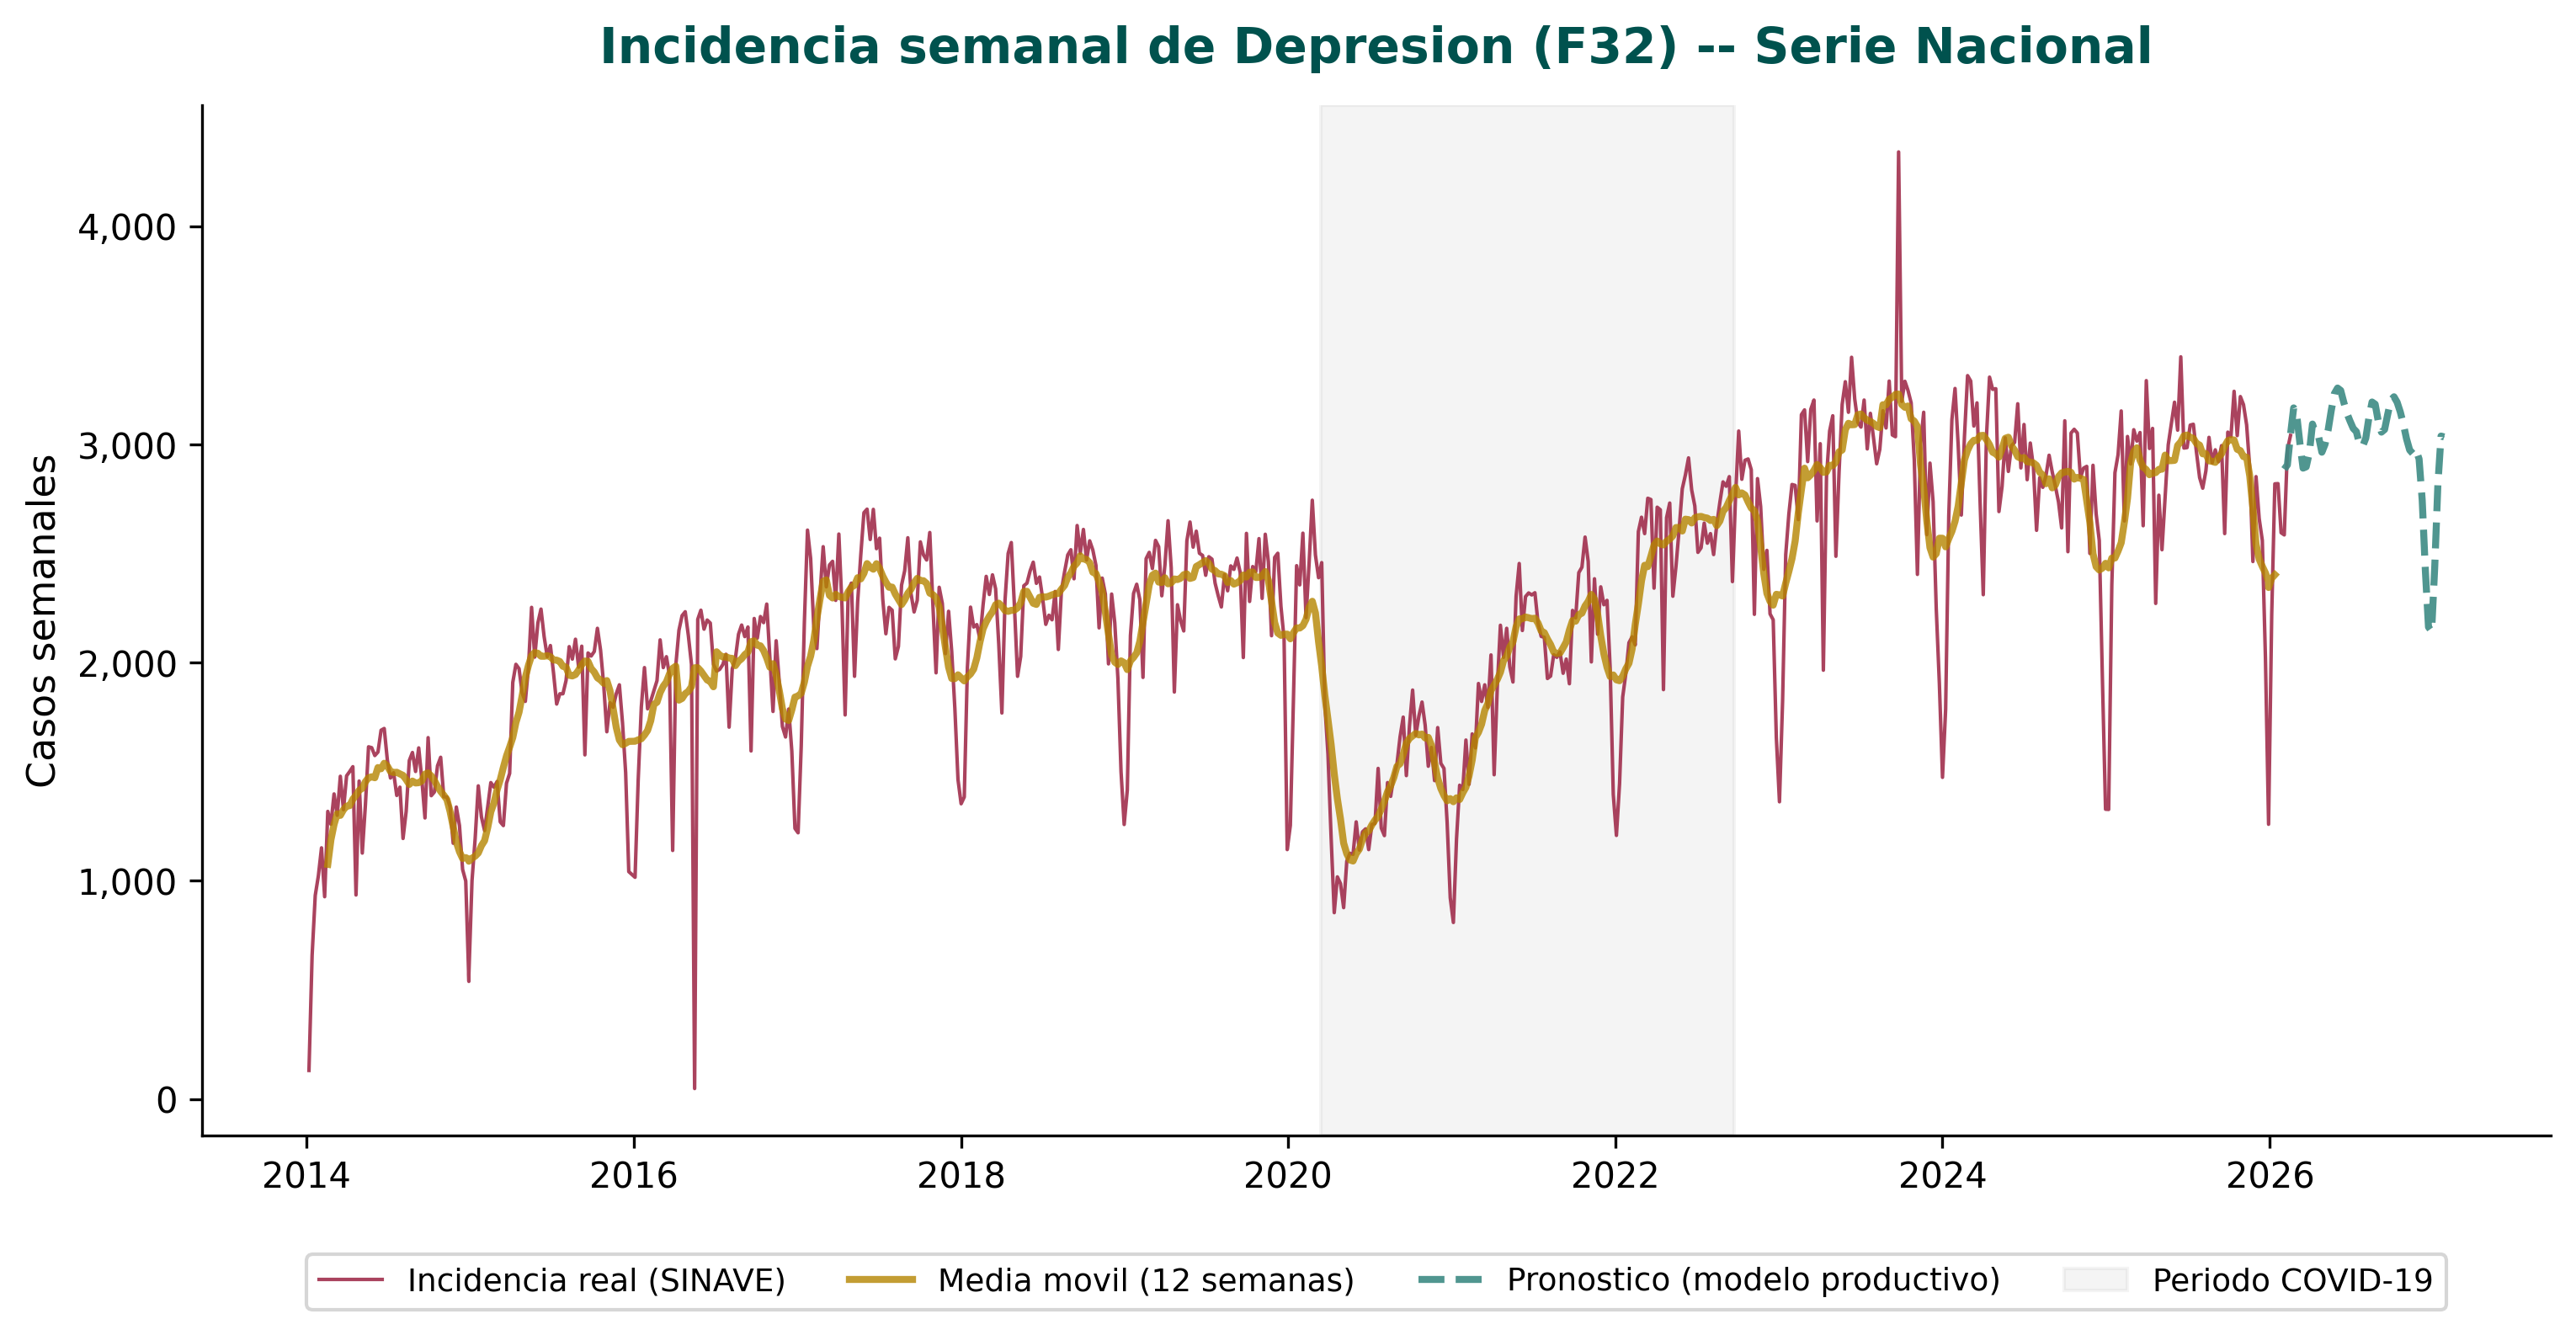
\includegraphics[width=1.15\textwidth]{eda_serie_temporal.png}}
\caption[Serie temporal de Depresión (F32) -- Nacional.]{Incidencia semanal de Depresión (F32) a nivel nacional, 2014--2025. Se observa una tendencia creciente pre-pandemia, la disrupción COVID-19 (franja sombreada, 2020--2022) y la recuperación posterior con un nuevo régimen de crecimiento.}
\label{fig:eda_serie}
\end{figure}

Como se observa en la \figref{fig:eda_serie}, la depresión presenta picos estacionales entre febrero y mayo, coincidiendo con el inicio del año escolar y laboral. La caída durante el periodo COVID-19 refleja una disminución en el reporte, no en la incidencia real. La recuperación post-pandemia muestra un nuevo régimen de crecimiento que supera los niveles pre-pandemia.

\begin{figure}[H]
\centering
\makebox[\textwidth][c]{%
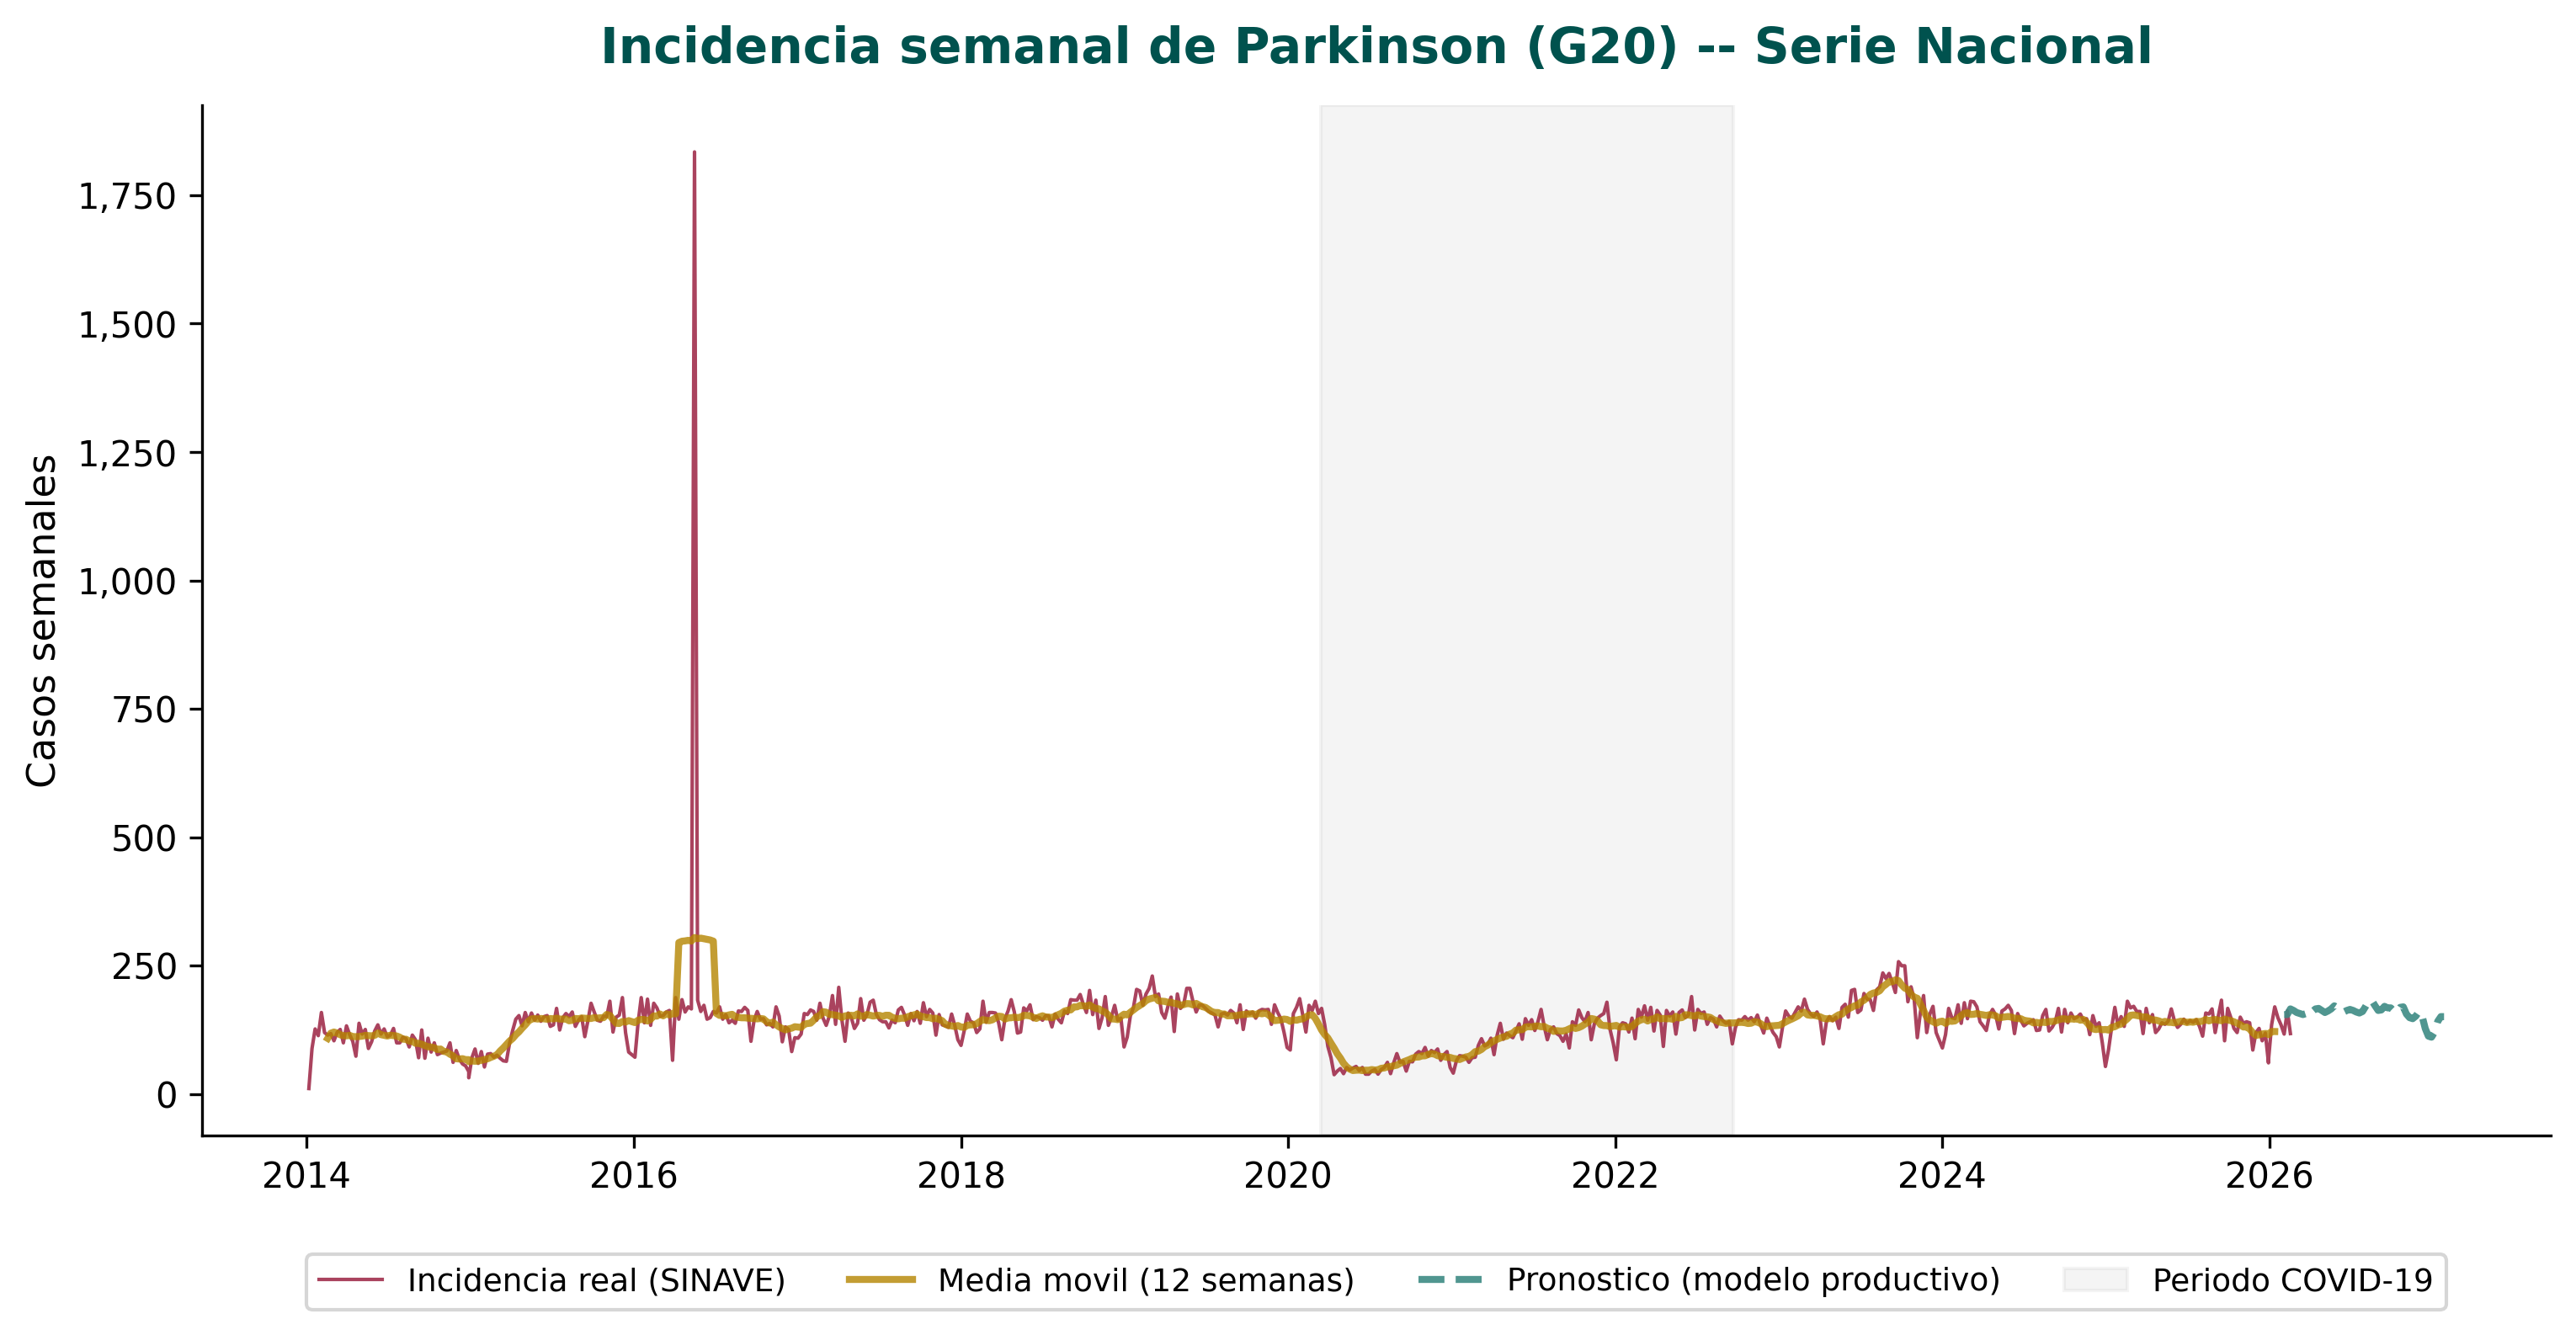
\includegraphics[width=1.15\textwidth]{eda_serie_parkinson.png}}
\caption[Serie temporal de Parkinson (G20) -- Nacional.]{Incidencia semanal de Parkinson (G20) a nivel nacional, 2014--2025. Se observa una tendencia de crecimiento sostenido consistente con el envejecimiento poblacional, con una estacionalidad menos marcada que la depresión.}
\label{fig:eda_parkinson}
\end{figure}

El Parkinson (\figref{fig:eda_parkinson}) muestra una estacionalidad menos marcada pero con incrementos sostenidos año tras año, consistente con el envejecimiento poblacional en México. La disrupción COVID-19 también afectó el reporte, aunque la recuperación fue más gradual.

\begin{figure}[H]
\centering
\makebox[\textwidth][c]{%
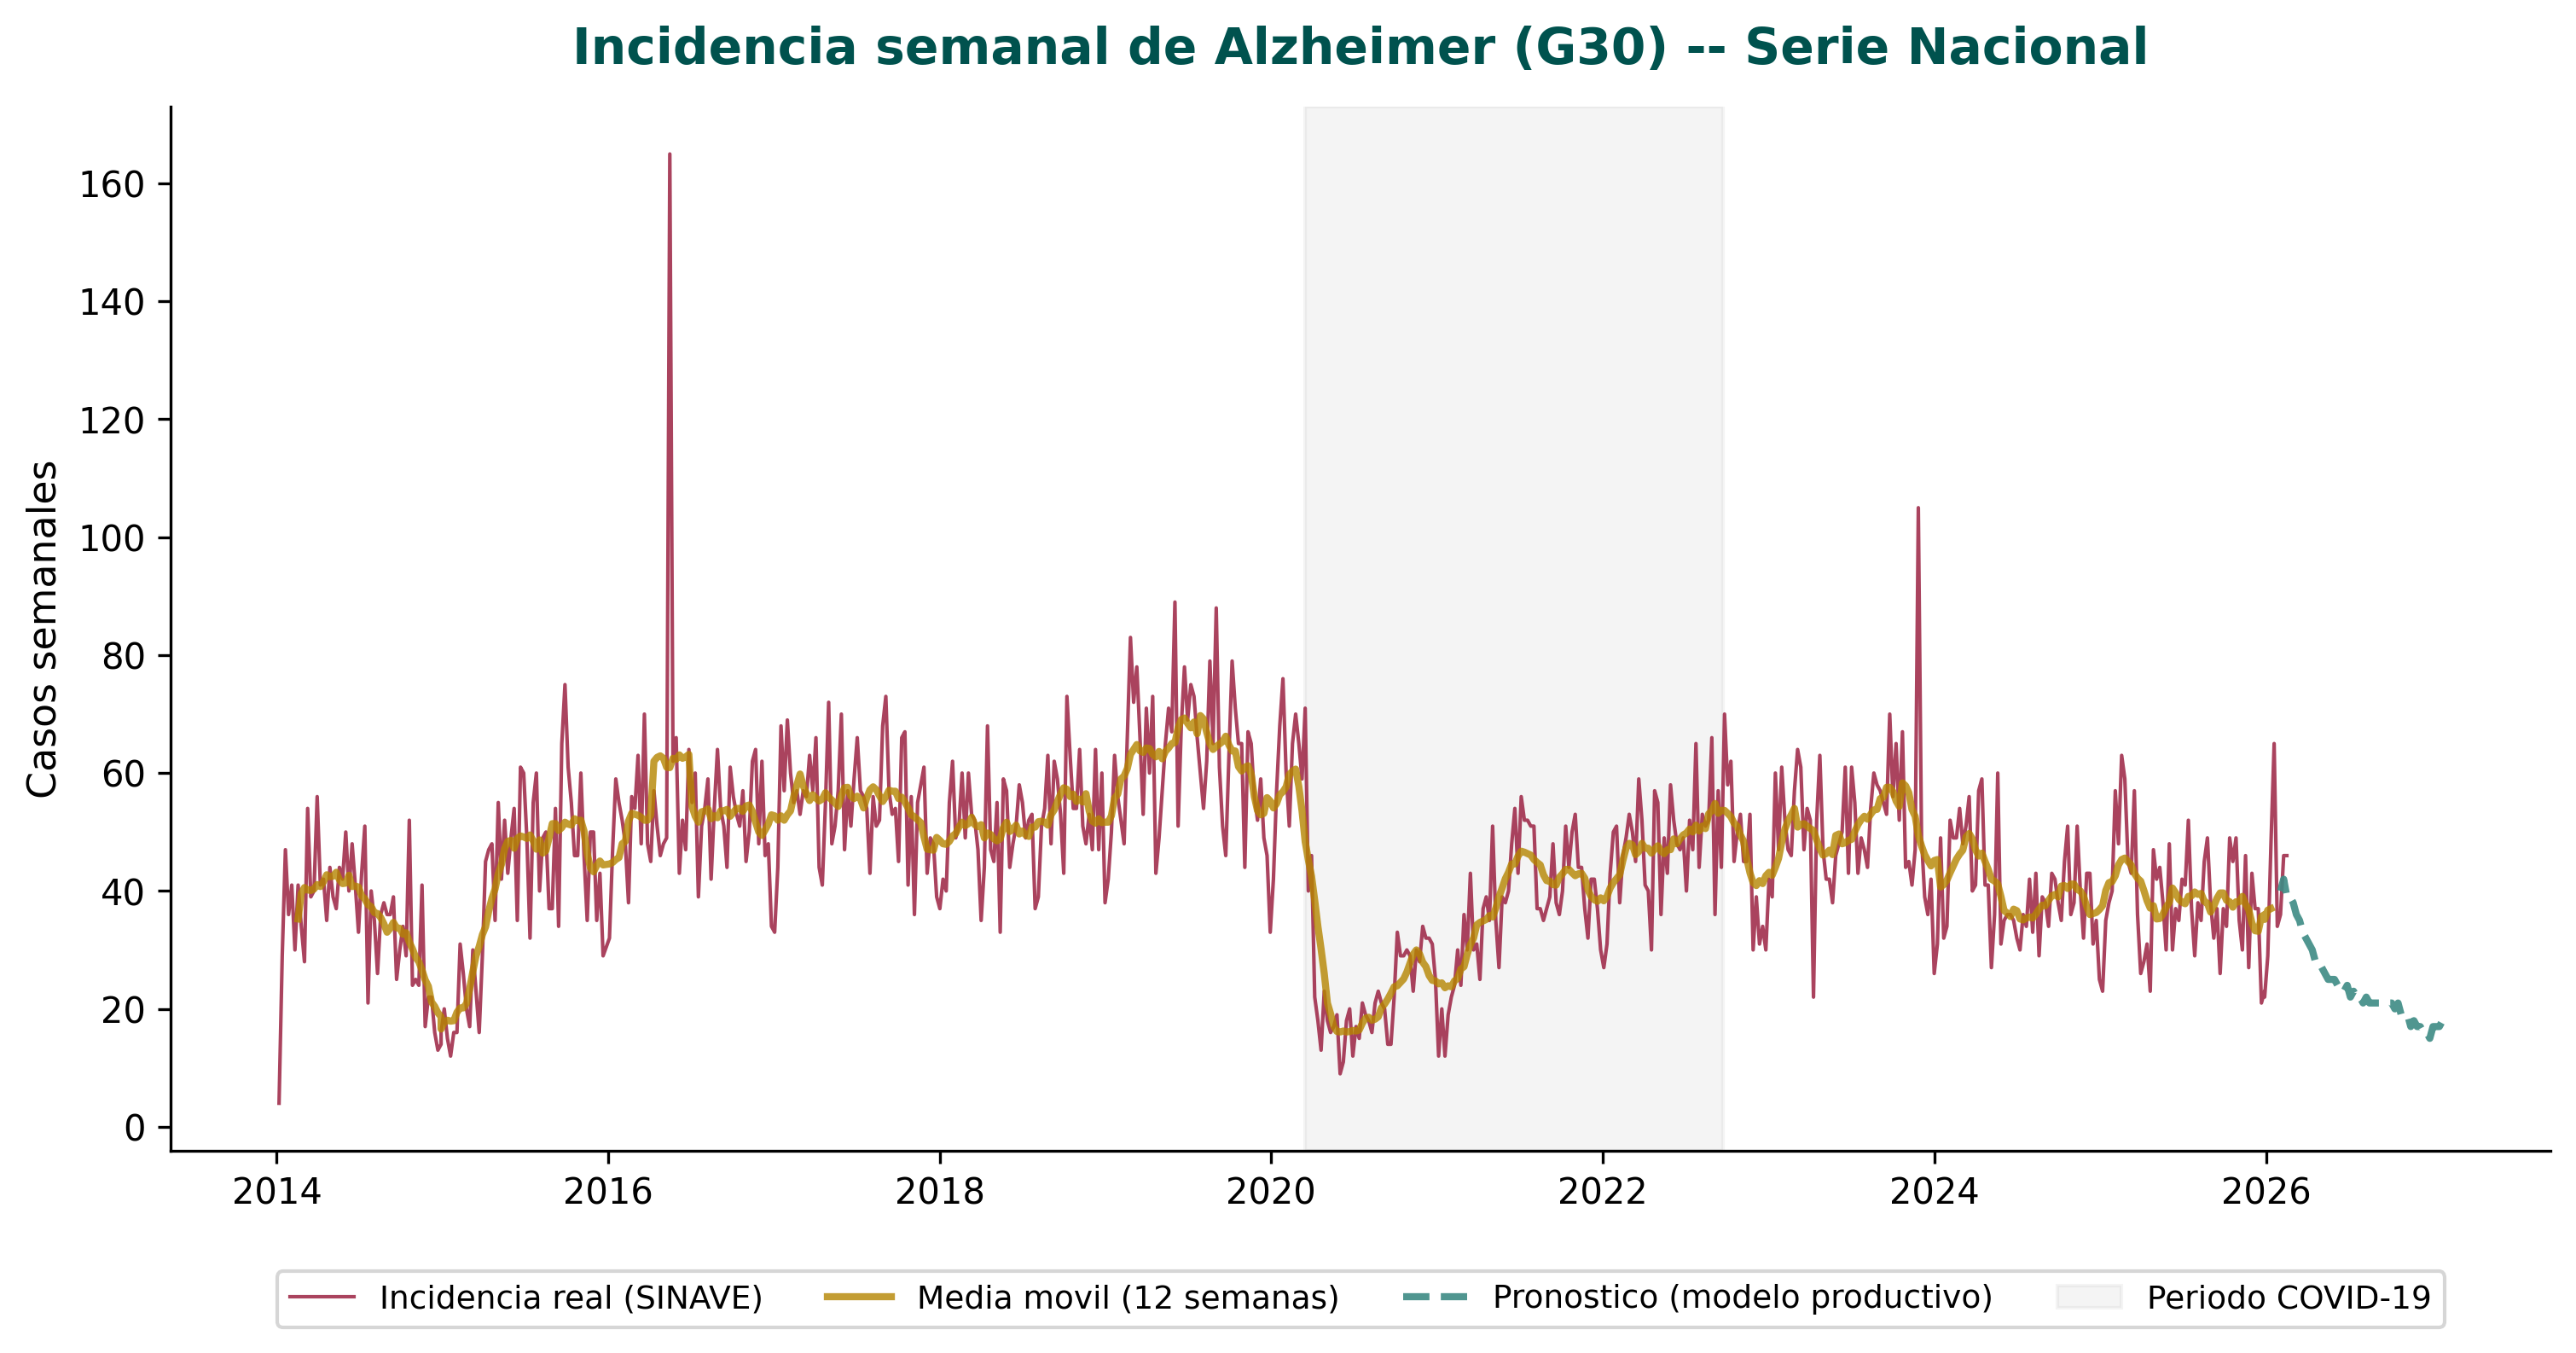
\includegraphics[width=1.15\textwidth]{eda_serie_alzheimer.png}}
\caption[Serie temporal de Alzheimer (G30) -- Nacional.]{Incidencia semanal de Alzheimer (G30) a nivel nacional, 2014--2025. La baja incidencia registrada genera alta volatilidad, con un punto de cambio estructural durante la pandemia.}
\label{fig:eda_alzheimer}
\end{figure}

El Alzheimer (\figref{fig:eda_alzheimer}) exhibe la mayor volatilidad de los tres padecimientos debido a su baja incidencia registrada (frecuentemente menor a 5~casos semanales en muchos estados). Esta característica genera un desafío estadístico particular para los modelos de pronóstico y explica la inflación del \smape{} en este padecimiento.

\subsection{El efecto COVID-19: disrupción, no desaparición}

El periodo 2020--2022 no refleja una disminución real en la incidencia de estas enfermedades, sino una \textbf{caída en el reporte} provocada por la centralización de los servicios de salud en la atención de la emergencia sanitaria. La Dra.~Ruth Perez-Hernandez confirmó que los patrones post-pandemia muestran una recuperación hacia las tendencias pre-pandemia, sin evidencia de un cambio epidemiológico permanente en la depresión y el Parkinson. Para Alzheimer, se adoptó una postura prudente al no concluir cambio de tendencia definitivo.

\subsection{Diferencial por género}

\begin{figure}[H]
\centering
\makebox[\textwidth][c]{%
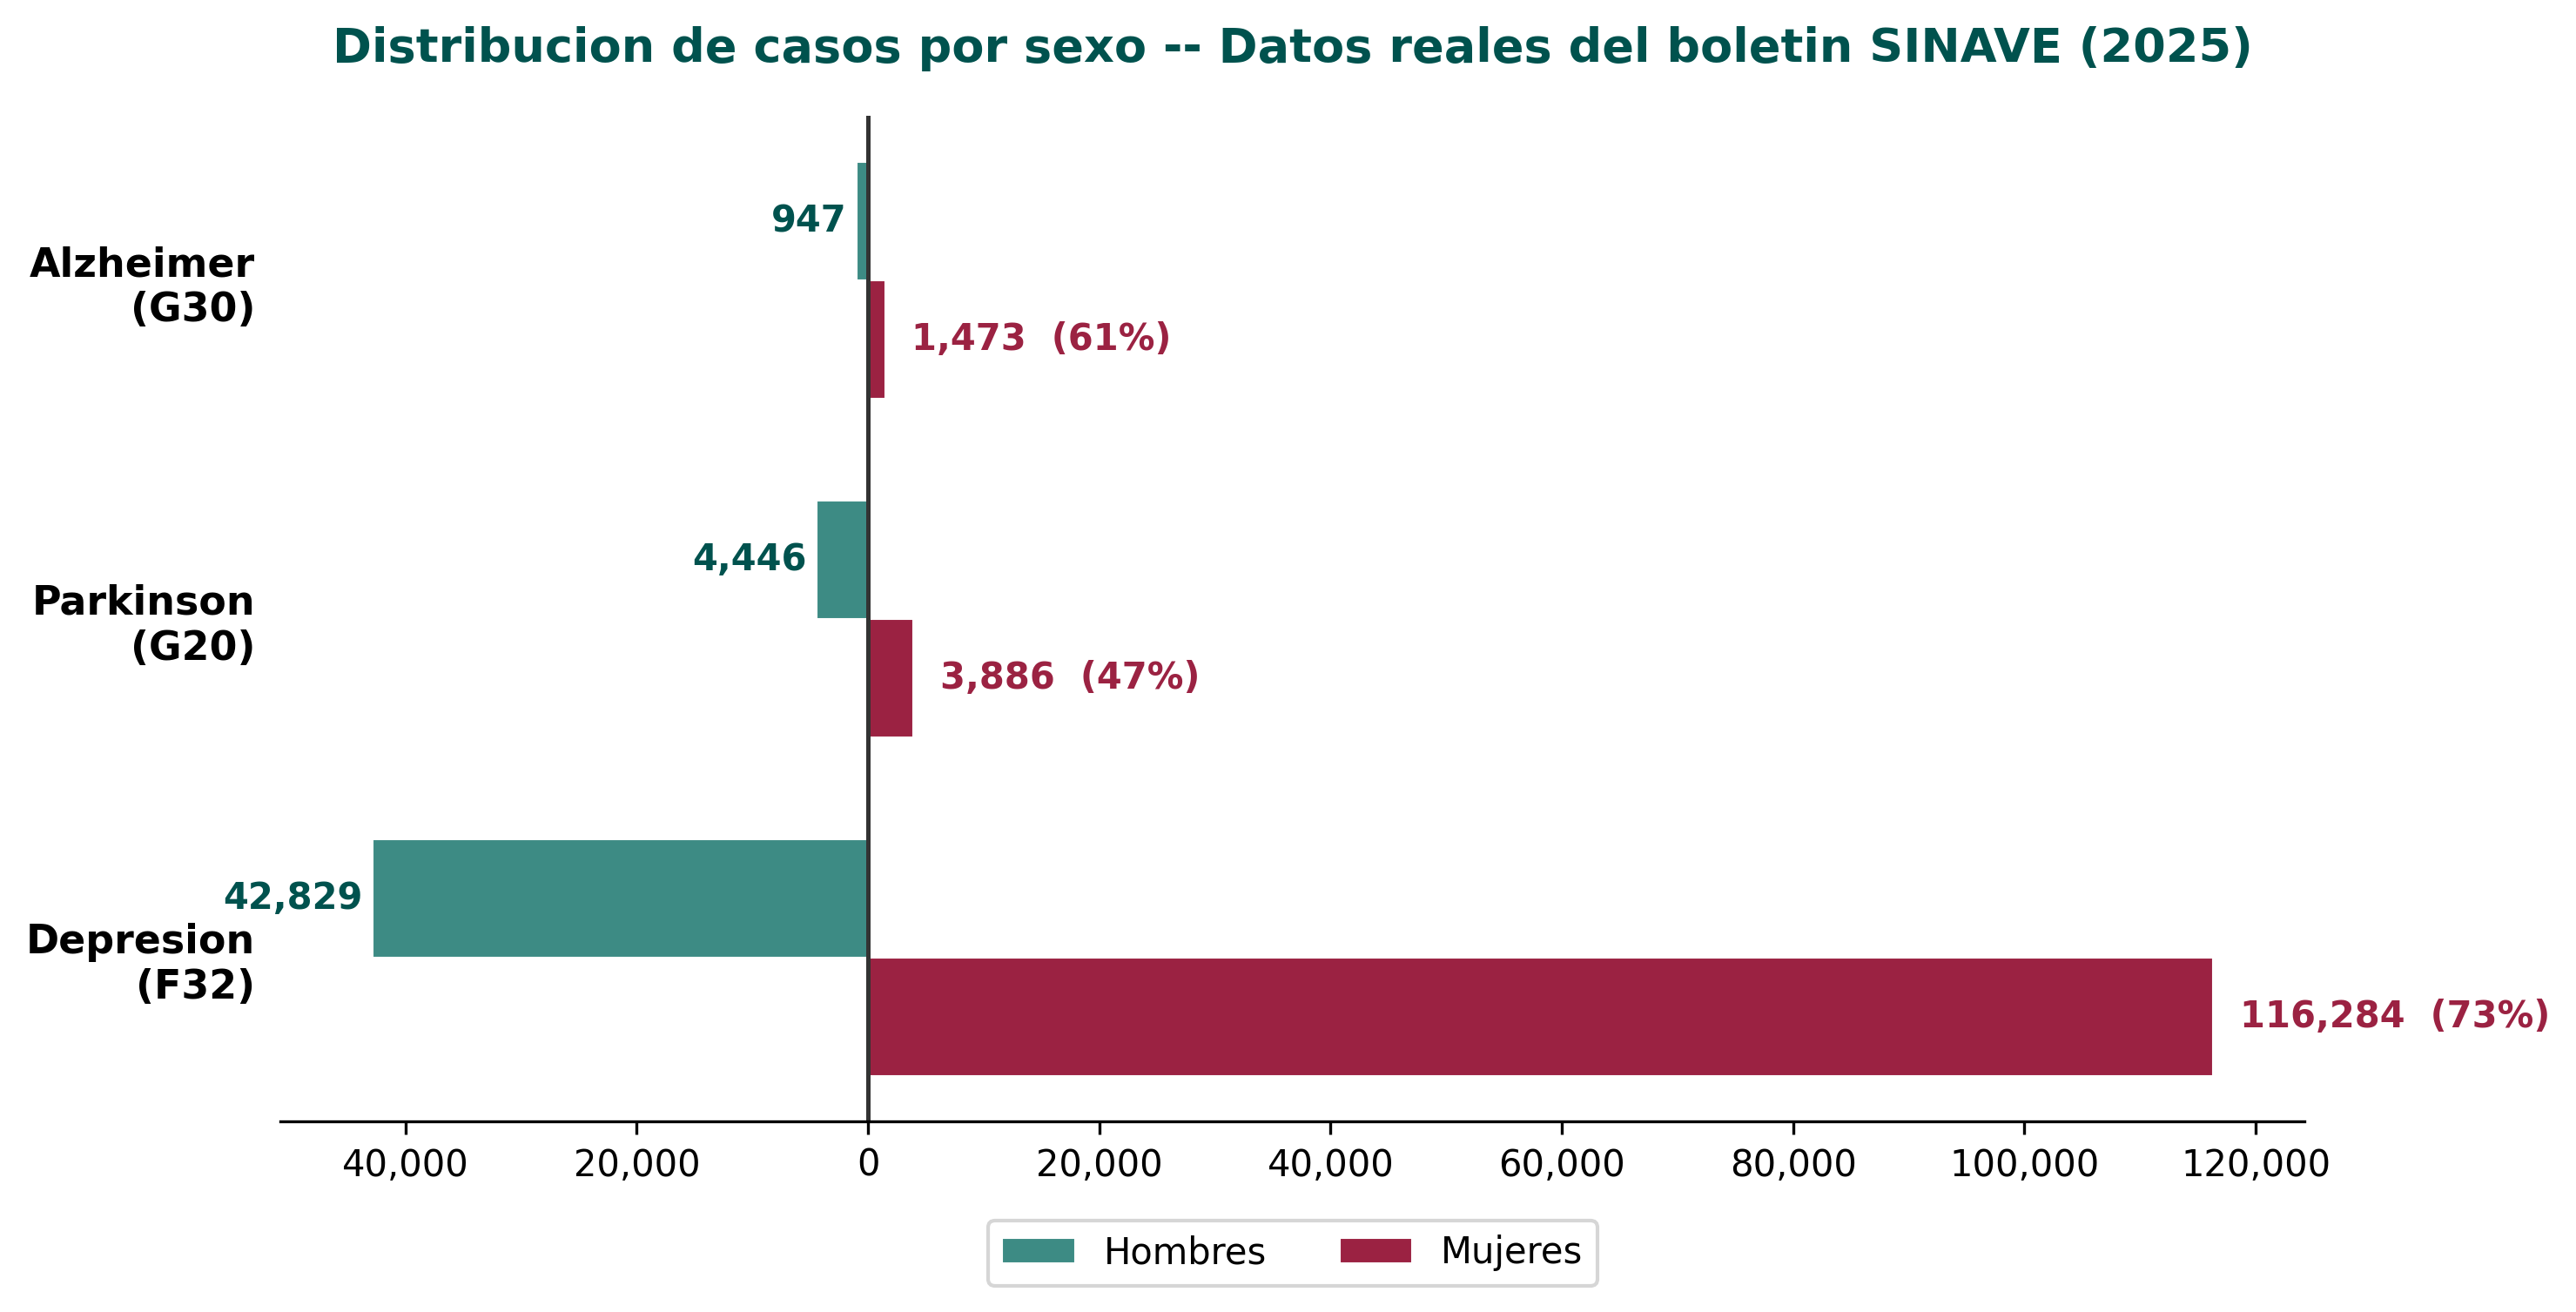
\includegraphics[width=1.05\textwidth]{eda_genero_butterfly.png}}
\caption[Distribución de casos por sexo (datos reales 2025).]{Distribución de casos acumulados por sexo y padecimiento según el boletín SINAVE 2025. En depresión, las mujeres representan el 73\% de los casos; en Alzheimer, el 61\%. Solo en Parkinson la distribución es prácticamente paritaria con ligera predominancia masculina (53\%).}
\label{fig:eda_genero}
\end{figure}

La \figref{fig:eda_genero} muestra la distribución real por sexo registrada en el boletín SINAVE durante 2025. Las mujeres representan el 73.1\% de los casos de depresión (116,284 vs.\ 42,829~casos acumulados), un diferencial que se mantiene en todas las entidades federativas y que la OMS atribuye a factores biológicos, hormonales y de acceso al diagnóstico. En Alzheimer, las mujeres también predominan con el 60.9\% de los casos (1,473 vs.\ 947), consistente con su mayor esperanza de vida. Solo en Parkinson la distribución es prácticamente paritaria: 53.4\% masculina (4,446 vs.\ 3,886), alineado con los factores de riesgo ocupacional y ambiental descritos en la literatura (OMS, 2022). Estos patrones, observados consistentemente en los datos históricos, justificaron la desagregación por sexo en las 333~series de producción: un modelo que ignore el género produciría pronósticos sesgados que no reflejan la realidad clínica.

\subsection{Heterogeneidad geográfica}

\begin{figure}[H]
\centering
\makebox[\textwidth][c]{%
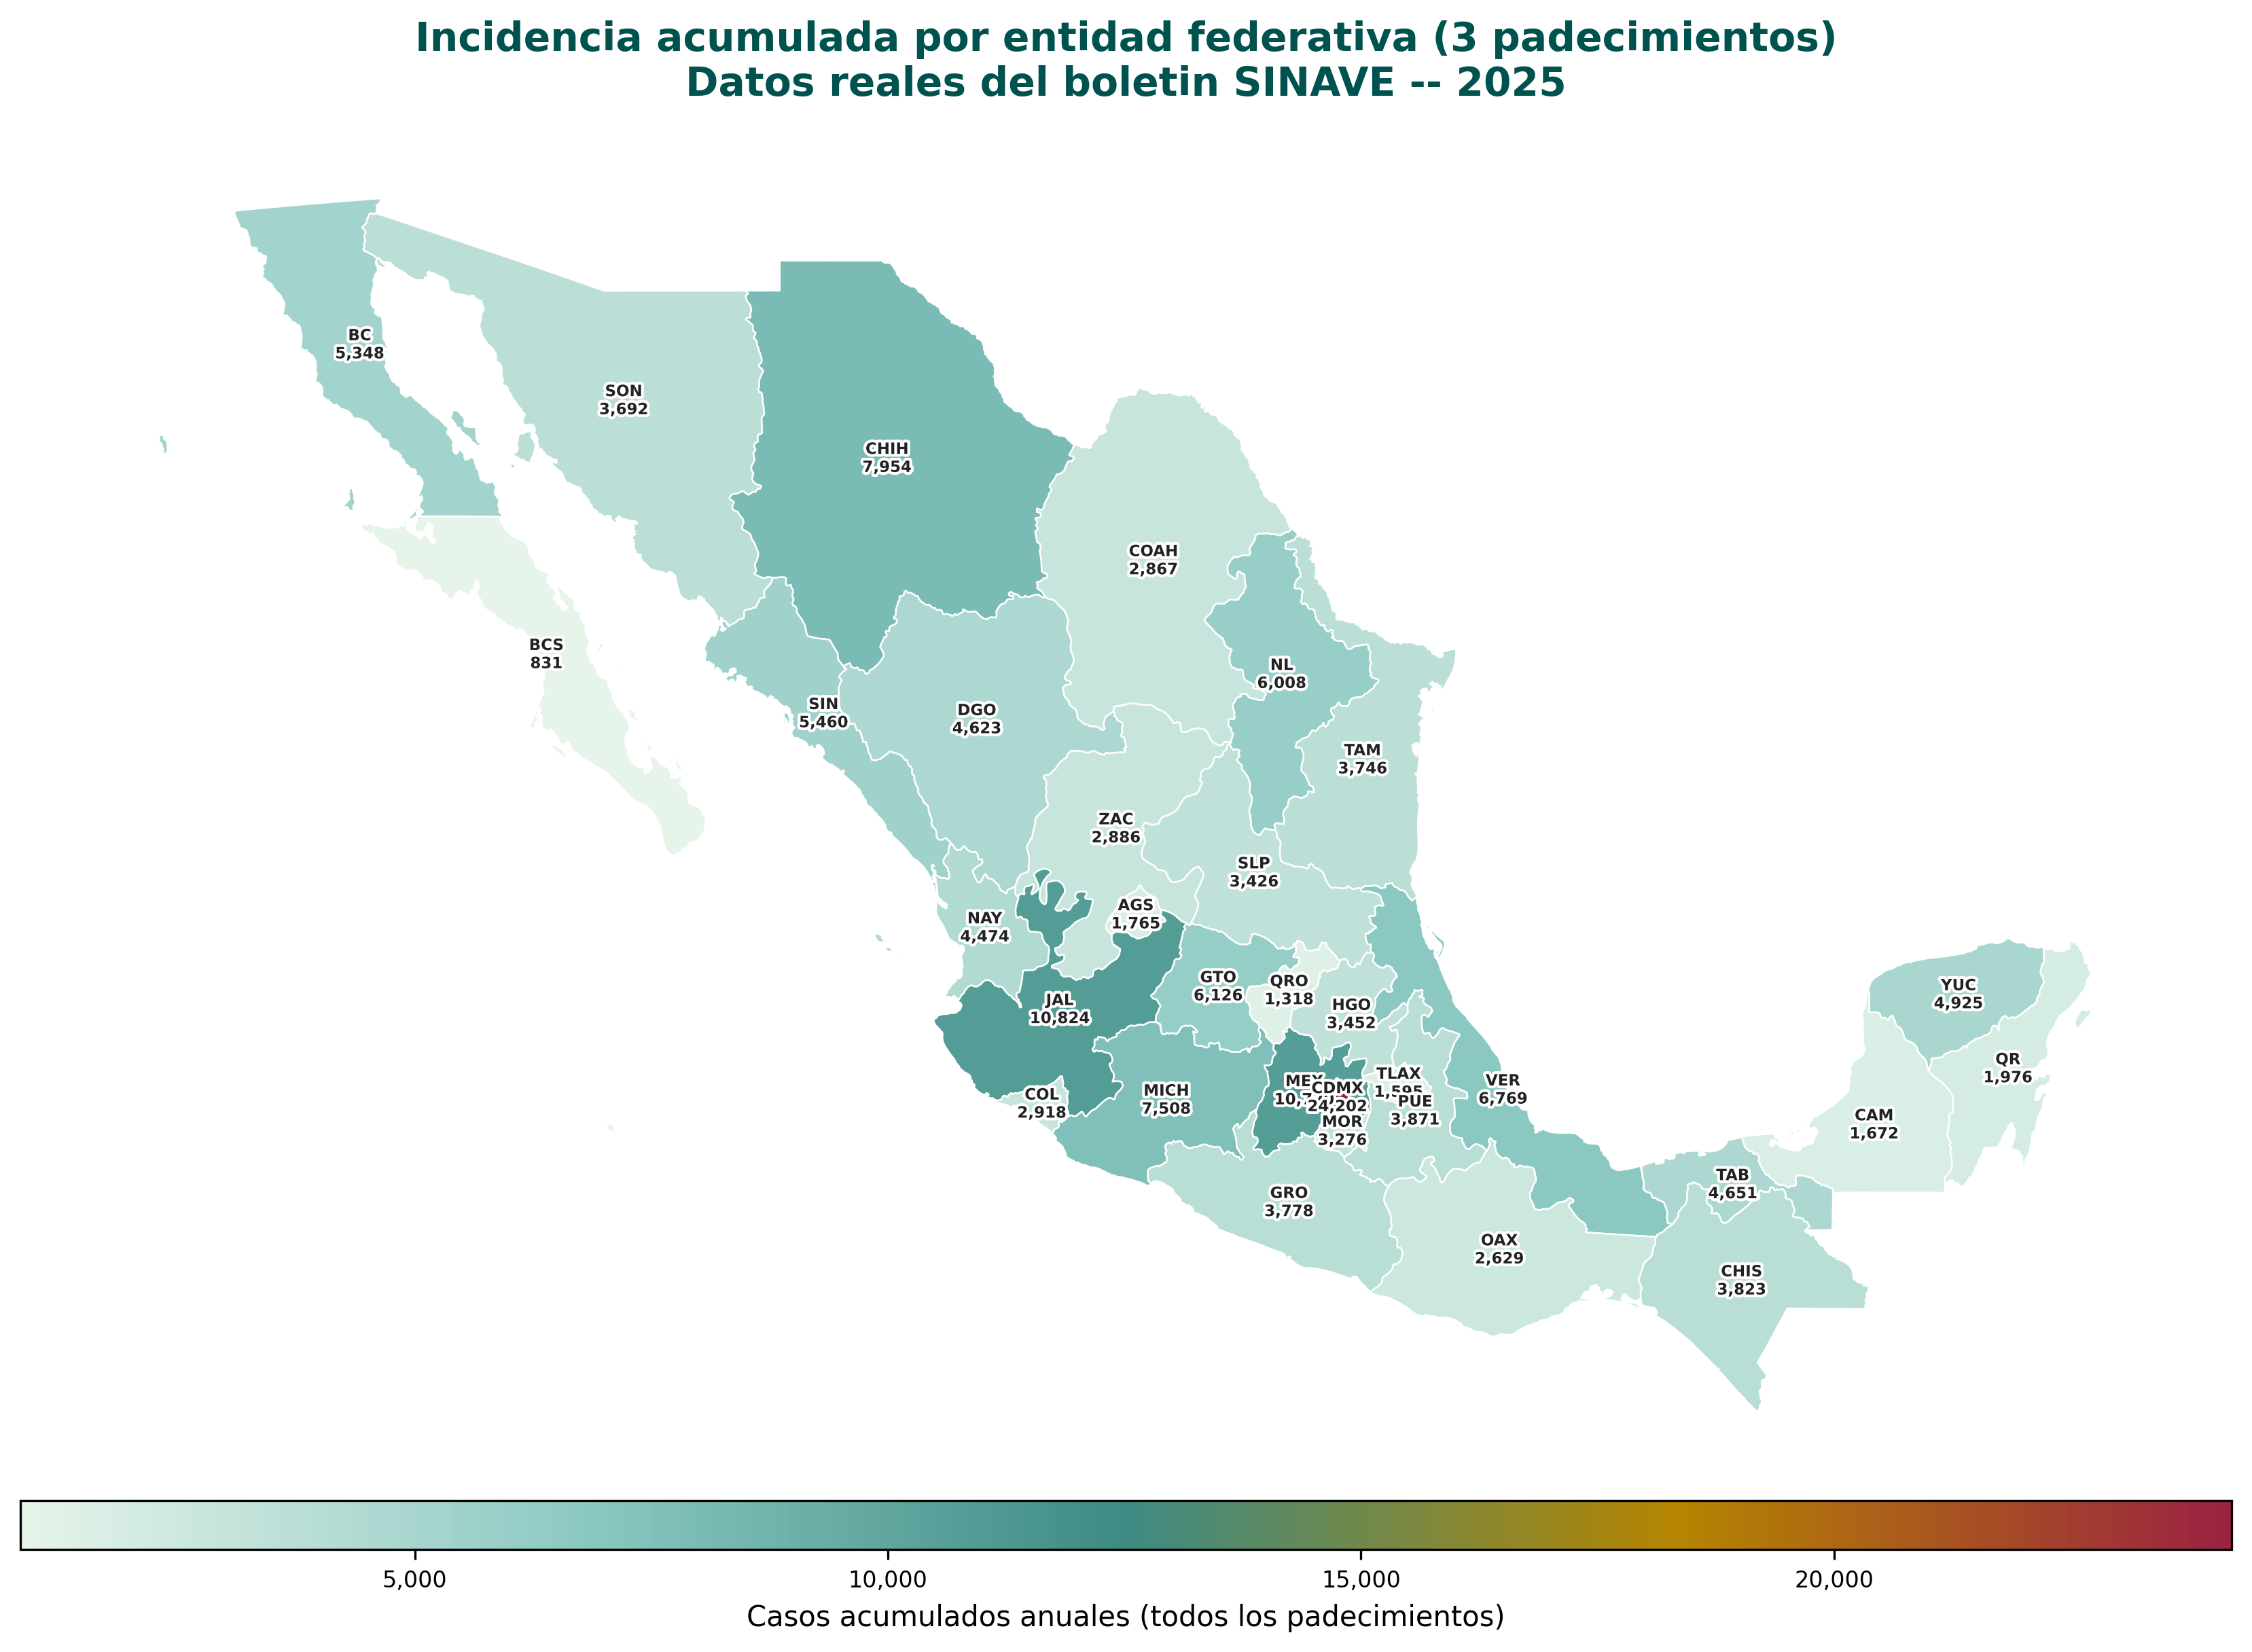
\includegraphics[width=1.05\textwidth]{eda_mapa_mexico.png}}
\caption[Mapa coroplético: incidencia por entidad federativa (2025).]{Distribución geográfica de la incidencia acumulada de los tres padecimientos por entidad federativa, según datos reales del boletín SINAVE 2025. La intensidad del color refleja el volumen total de casos reportados. Se observa una concentración marcada en el centro y occidente del país.}
\label{fig:eda_mapa}
\end{figure}

La \figref{fig:eda_mapa} revela que la carga de enfermedad no se distribuye uniformemente en el territorio nacional. Jalisco (10,824~casos), Estado de México (10,243), Chihuahua (7,954) y Michoacán (7,508) concentran los mayores volúmenes, mientras que estados como Baja California Sur (831), Querétaro (1,318) y Campeche (1,672) presentan cifras significativamente menores. Esta heterogeneidad responde a factores como densidad poblacional, capacidad de detección del sistema de salud y disponibilidad de especialistas.

Un hallazgo relevante del EDA es el \textbf{reporte intermitente} en estados de baja incidencia. La Tabla~\ref{tab:alerta_ceros} identifica las entidades con más del 50\% de semanas epidemiológicas sin casos reportados durante 2025.

\begin{table}[H]
\centering
\caption{Alerta de calidad: entidades con reporte intermitente (2025)}
\label{tab:alerta_ceros}
\small
\renewcommand{\arraystretch}{1.15}
\begin{tabularx}{\textwidth}{l l r r r}
\toprule
\rowcolor{teal!90} \textcolor{white}{\textbf{Padecimiento}} & \textcolor{white}{\textbf{Entidad}} & \textcolor{white}{\textbf{Casos anuales}} & \textcolor{white}{\textbf{Sem. en cero}} & \textcolor{white}{\textbf{\% sin reporte}} \\
\midrule
\rowcolor{lightred} Alzheimer & Tlaxcala          &   5 & 48/53 & \textbf{\textcolor{burgundy}{91\%}} \\
\rowcolor{lightred} Alzheimer & Querétaro         &  10 & 45/53 & \textbf{\textcolor{burgundy}{85\%}} \\
\rowcolor{lightred} Alzheimer & San Luis Potosí   &  10 & 43/53 & \textbf{\textcolor{burgundy}{81\%}} \\
\rowcolor{lightred} Alzheimer & Zacatecas         &  12 & 42/53 & \textbf{\textcolor{burgundy}{79\%}} \\
\rowcolor{lightyellow} Alzheimer & Aguascalientes  &  15 & 39/53 & \textbf{\textcolor{gold}{74\%}} \\
\rowcolor{lightyellow} Alzheimer & Baja California Sur & 18 & 38/53 & \textbf{\textcolor{gold}{72\%}} \\
\rowcolor{lightyellow} Alzheimer & Campeche        &  19 & 38/53 & \textbf{\textcolor{gold}{72\%}} \\
\rowcolor{lightyellow} Alzheimer & Quintana Roo    &  18 & 38/53 & \textbf{\textcolor{gold}{72\%}} \\
\rowcolor{lightyellow} Alzheimer & Yucatán         &  19 & 37/53 & \textbf{\textcolor{gold}{70\%}} \\
Alzheimer & Tabasco            &  25 & 33/53 & 62\% \\
Alzheimer & Guerrero           &  37 & 30/53 & 57\% \\
Alzheimer & Hidalgo            &  36 & 30/53 & 57\% \\
Alzheimer & Chiapas            &  41 & 27/53 & 51\% \\
\midrule
Parkinson & Tlaxcala           &  31 & 30/53 & 57\% \\
Parkinson & Nayarit            &  39 & 29/53 & 55\% \\
\bottomrule
\end{tabularx}
\vspace{0.2cm}
\begin{flushleft}
\footnotesize\textit{Fuente: Boletín Epidemiológico SINAVE, 53~semanas epidemiológicas de 2025.
Las filas en \colorbox{lightred}{\scriptsize rojo} indican estados con $\geq$79\% de semanas sin reporte;
en \colorbox{lightyellow}{\scriptsize amarillo}, entre 70\% y 74\%.
El reporte intermitente puede reflejar subregistro, falta de especialistas o baja prevalencia real.}
\end{flushleft}
\end{table}

Para Alzheimer, 13~entidades reportan cero casos en más del 50\% de las semanas epidemiológicas; Tlaxcala alcanza el 91\% de semanas sin reporte (solo 5~casos anuales). En Parkinson, Tlaxcala y Nayarit superan el 50\% de semanas en cero. Este patrón constituye una señal de alerta para la calidad del dato que el sistema debe manejar con robustez.

\begin{figure}[H]
\centering
\makebox[\textwidth][c]{%
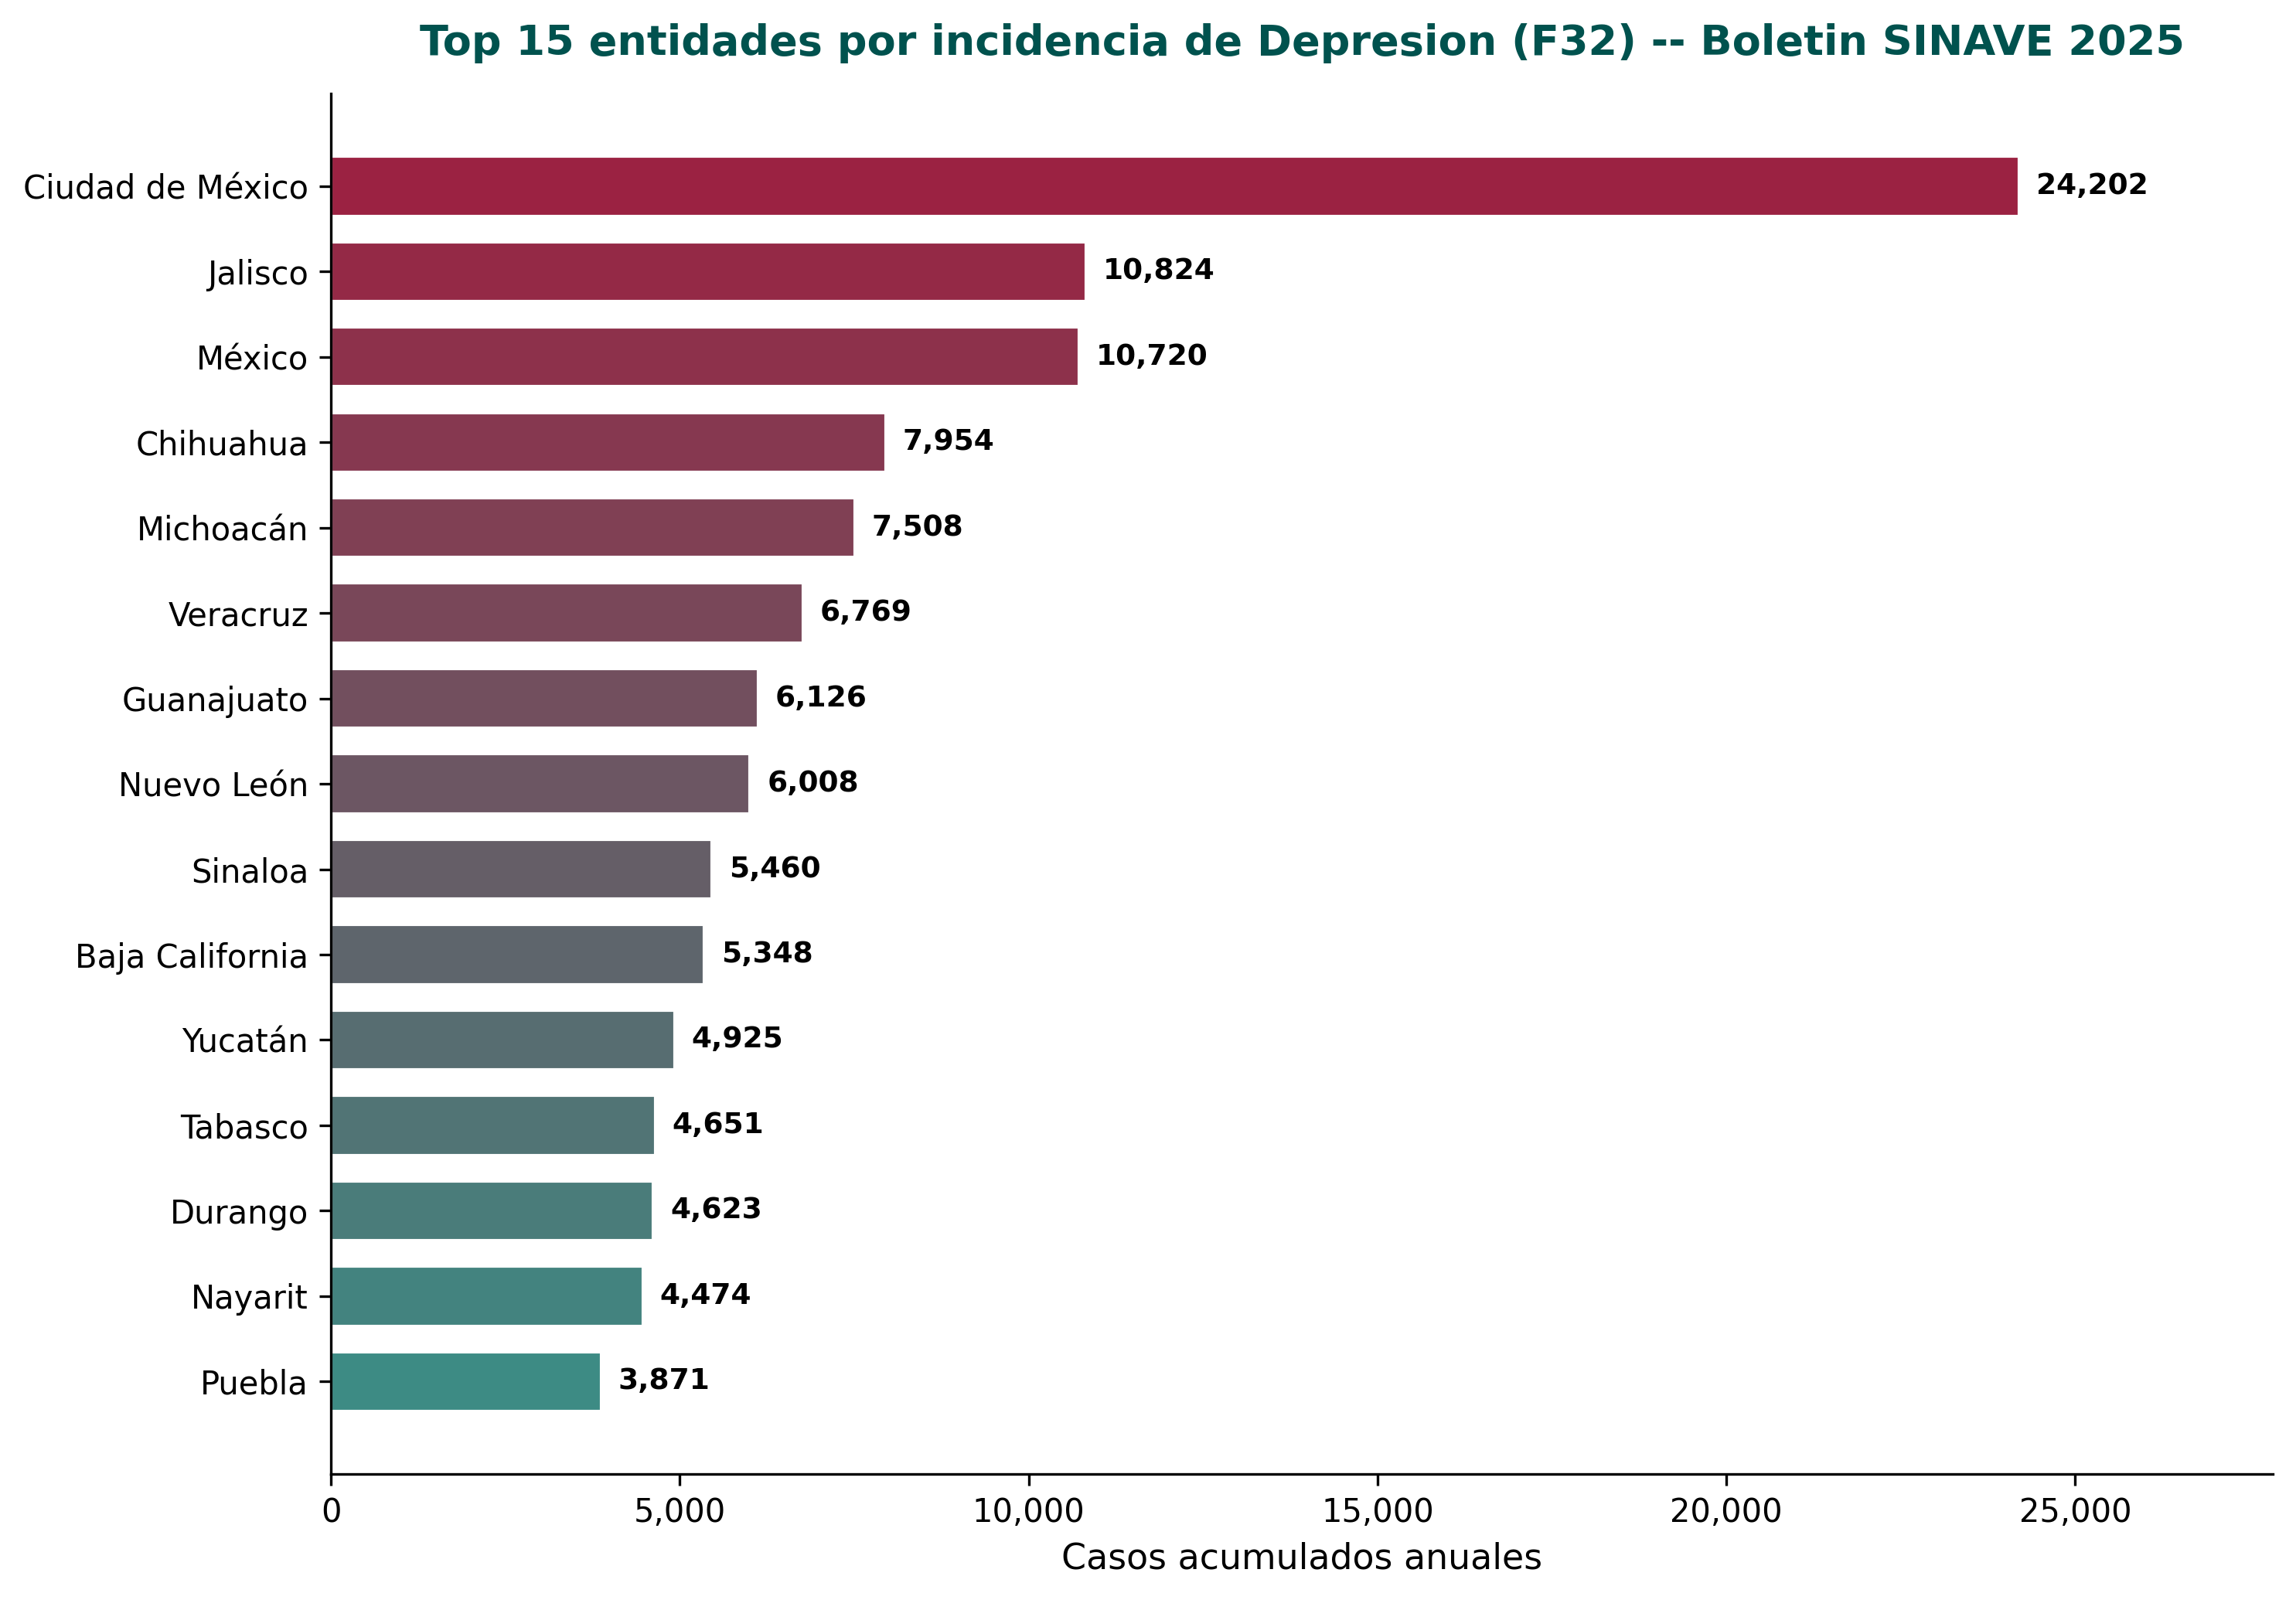
\includegraphics[width=1.15\textwidth]{eda_heatmap_geografico.png}}
\caption[Top 15 entidades por incidencia de Depresión (F32).]{Las 15~entidades con mayor incidencia acumulada de Depresión (F32) según el boletín SINAVE 2025. Ciudad de México lidera con 24,202~casos, seguida por Jalisco (10,824) y Estado de México (10,720). La concentración en el centro y norte del país refleja tanto la distribución poblacional como la capacidad de detección del sistema de salud.}
\label{fig:eda_geografico}
\end{figure}

Para las entidades con series de muy baja incidencia (menos de 5~casos semanales) o reporte intermitente, el sistema implementa una estrategia de \textbf{agrupación regional}: en lugar de entrenar un modelo individual que carecería de datos suficientes, se asigna el modelo de la región geográfica correspondiente, garantizando pronósticos estables aun en las series más desafiantes.

% ============================================================
% 4. INGENIERIA DE CARACTERISTICAS
% ============================================================
\newpage
\section{Ingeniería de características}\label{sec:features}

Antes de alimentar cualquier motor de pronóstico, las series temporales crudas del boletín SINAVE atraviesan un pipeline de ingeniería de características diseñado para maximizar la señal predictiva y minimizar el ruido. Este proceso transforma los conteos semanales brutos en un espacio de features rico que captura la dinámica temporal, la estacionalidad, la volatilidad y el contexto demográfico de cada serie.

\begin{figure}[H]
\centering
\makebox[\textwidth][c]{%
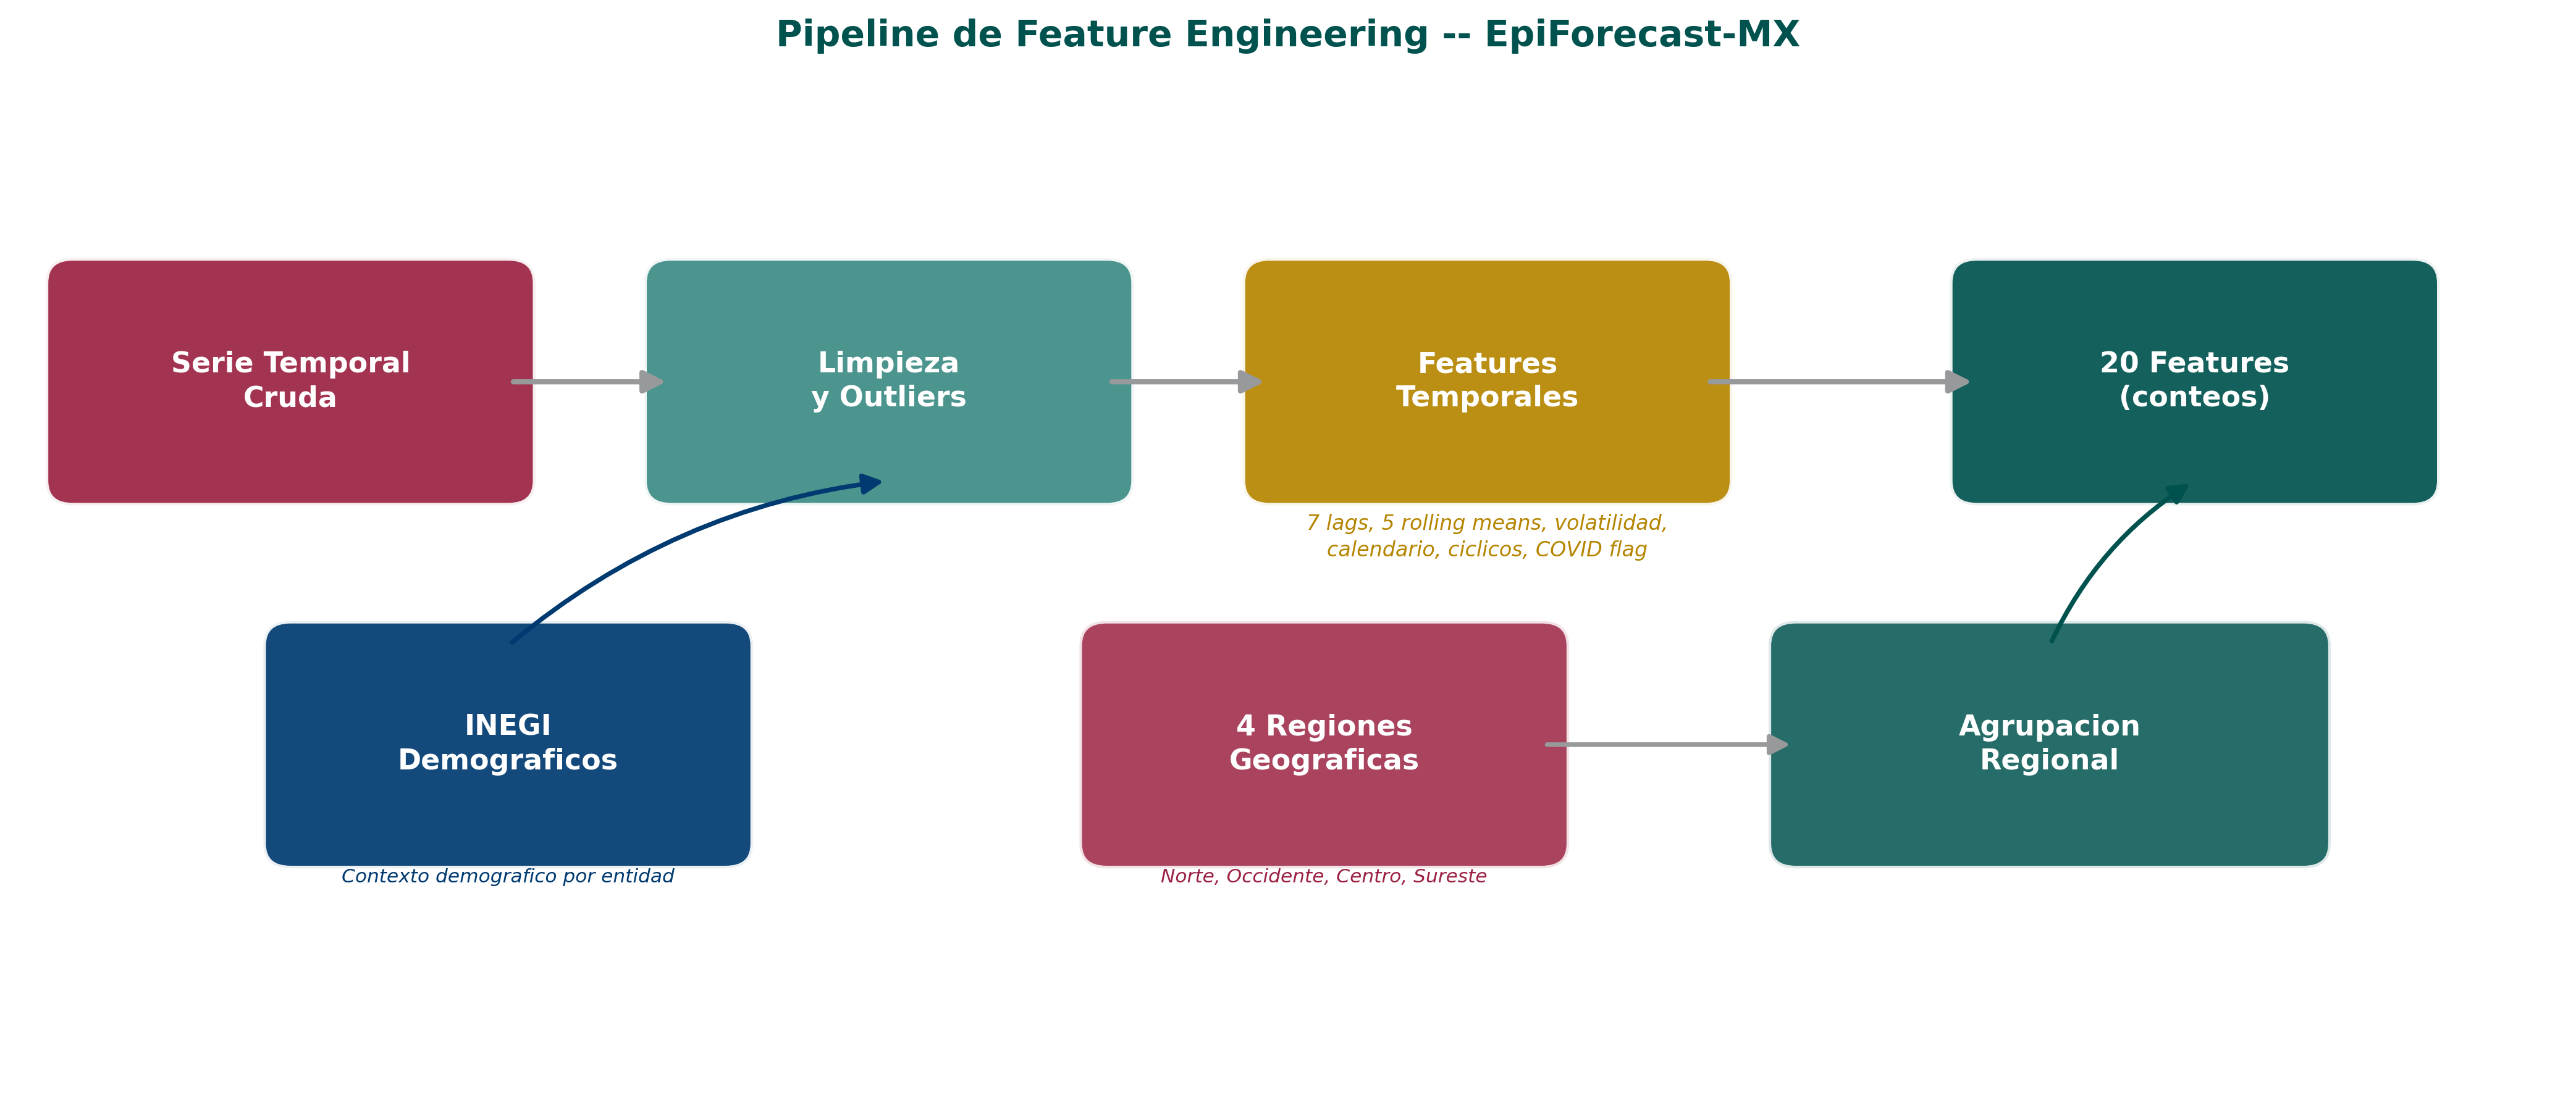
\includegraphics[width=1.15\textwidth]{feature_engineering_pipeline.png}}
\caption[Pipeline de ingeniería de características.]{Pipeline de transformación de datos: desde la serie temporal cruda hasta las 20~features que alimentan los modelos de machine learning. Los datos demográficos del INEGI enriquecen el contexto, y la agrupación regional proporciona series robustas para entidades de baja incidencia.}
\label{fig:feature_pipeline}
\end{figure}

\subsection{Target: conteos absolutos, no tasas}

Una decisión de diseño fundamental fue definir el target como \textbf{conteos absolutos de casos} (número entero de incidentes semanales), no como tasa por 100,000~habitantes. En versiones previas del sistema se experimentó con normalización por tasa poblacional utilizando datos del INEGI, pero el análisis posterior reveló que los conteos absolutos producían pronósticos más estables y directamente interpretables para la planificación operativa. La Dra.~Grettel Barcelo validó esta decisión: \textit{``Usar los casos directamente puede ser más conveniente, especialmente si el objetivo es asociarlo con la planeación operativa. Además, la población es constante y los modelos son independientes por entidad.''} Las visualizaciones del dashboard sí incluyen una vista normalizada por 100,000~habitantes (a solicitud de la Dra.~Ruth Pérez Hernández), pero el modelado y la selección de motor operan sobre conteos absolutos.

Los motores Ensemble y Stacking operan nativamente sobre conteos absolutos. Prophet y DeepAR aplican internamente una normalización temporal (escalamiento por media en el caso de GluonTS), pero sus predicciones finales se desnormalizan y redondean a enteros antes de entrar al sistema de selección, garantizando que todas las comparaciones entre motores se realizan en la misma escala: \textbf{casos enteros por semana}.

\subsection{Features temporales y de autocorrelación}

El motor Ensemble construye un espacio de 20~features explícitas a partir de cada serie, organizadas en seis familias:

\begin{table}[H]
\centering
\caption{Catálogo de features del motor Ensemble (Prophet + XGBoost)}
\label{tab:features_catalogo}
\small
\renewcommand{\arraystretch}{1.15}
\begin{tabularx}{\textwidth}{l l X}
\toprule
\rowcolor{teal!90} \textcolor{white}{\textbf{Familia}} & \textcolor{white}{\textbf{Features}} & \textcolor{white}{\textbf{Descripción}} \\
\midrule
Lags & \texttt{lag\_\{1,2,4,8,13,26,52\}} & Autocorrelación a 1~semana, 1~mes, trimestre, semestre y año \\
\rowcolor{lightgreen} Medias móviles & \texttt{roll\_\{4,8,12,26,52\}} & Tendencia suavizada a distintas escalas temporales \\
Volatilidad & \texttt{roll\_std\_13} & Desviación estándar trimestral; mide la estabilidad de la serie \\
\rowcolor{lightgreen} Calendario & \texttt{month}, \texttt{week\_of\_year} & Componentes discretos del calendario \\
Cíclicos & \texttt{sin\_week}, \texttt{cos\_week} & Codificación trigonométrica: $\sin(2\pi \cdot \text{sem}/52)$, $\cos(2\pi \cdot \text{sem}/52)$ \\
\rowcolor{lightgreen} Tasa de cambio & \texttt{roc\_4}, \texttt{roc\_52} & Momentum a 1~mes y 1~año \\
Régimen & \texttt{covid\_flag} & Indicador binario del periodo pandémico (mar-2020 a sep-2022) \\
\bottomrule
\end{tabularx}
\end{table}

Todas las features de ventana deslizante se calculan sobre datos desplazados un periodo (\texttt{shift(1)}) para evitar fuga de información (data leakage), garantizando que el modelo nunca observe la semana que intenta predecir.

\subsection{Tratamiento de outliers y agrupación regional}

Los valores atípicos se detectan mediante z-score (umbral de 3$\sigma$) aplicado por grupo de padecimiento y entidad, y se reemplazan por la mediana del grupo. Para entidades con incidencia demasiado baja para entrenar modelos individuales robustos, el sistema agrupa las 32~entidades en cuatro regiones geográficas (Norte, Occidente, Centro y Sureste) y entrena un modelo regional que sirve como respaldo.

\subsection{Adaptaciones por motor}

No todos los modelos consumen las mismas features ni procesan los datos de la misma manera:

\begin{itemize}
  \item \textbf{Prophet} genera internamente su descomposición aditiva (tendencia, estacionalidad Fourier de orden~10, régimen COVID) sin features explícitas. No requiere el espacio de 20~features.
  \item \textbf{DeepAR} aprende representaciones latentes a través de sus capas LSTM sobre las 333~series simultáneamente. GluonTS aplica un escalamiento interno por media (\textit{mean scaling}) que normaliza cada serie a su propia escala, facilitando el aprendizaje cruzado entre series de magnitudes dispares.
  \item \textbf{Ensemble} consume las 20~features completas de la Tabla~\ref{tab:features_catalogo} directamente sobre conteos absolutos, permitiendo que XGBoost capture interacciones no lineales entre lags, momentum y volatilidad.
  \item \textbf{Stacking} utiliza un subconjunto compacto de 3~features trigonométricas ($\sin_{\text{sem}}$, $\cos_{\text{sem}}$, tendencia lineal) para su experto LightGBM, mientras Prophet y ETS operan con sus propias descomposiciones internas.
\end{itemize}

% ============================================================
% 5. MODELOS Y ELECCION DEL MODELO FINAL
% ============================================================
\newpage
\section{Estrategia multi-motor y selección del modelo}\label{sec:modelos}

\subsection{Por qué cuatro motores en lugar de uno}

La decisión de implementar una arquitectura multi-motor responde tanto a la evidencia empírica acumulada en más de cinco décadas de investigación en pronósticos como a la experiencia directa del proyecto. Durante la Fase~I, el equipo anterior evaluó modelos de machine learning (en particular ensambles basados en árboles de decisión como Random Forest y XGBoost), incorporando ingeniería de características orientada a capturar dependencias temporales (variables de rezago, componentes de tendencia y estacionalidad). Sin embargo, estos enfoques mostraron una \textbf{acumulación progresiva del error bajo un esquema de pronóstico recursivo} a múltiples pasos: a medida que el horizonte avanzaba, los lags pasaban de ser valores reales a predicciones, degradando la calidad exponencialmente. También se probaron redes LSTM, que sufrieron sobreajuste por la cantidad limitada de datos disponibles. La conclusión de la Fase~I fue que \textit{``ningún enfoque de machine learning resultó conveniente; los mejores resultados se obtuvieron con modelos clásicos de series de tiempo''} (Prophet como ganador).

La Fase~II parte de esta lección, pero no la repite: nuestro motor Ensemble \textbf{no} utiliza XGBoost como modelo recursivo autónomo, sino como corrector de residuos de Prophet (véase \S\ref{sec:ensemble}), eliminando la acumulación de error que plagó la Fase~I.

A nivel teórico, el principio está formalizado por Wolpert (1997) como el \textit{No Free Lunch Theorem}: no existe un algoritmo universalmente superior; el rendimiento depende de la estructura particular de cada problema. Las competencias M de Makridakis lo han confirmado de manera contundente:

\begin{itemize}
  \item En la \textbf{competencia M4} (100,000~series, 61~métodos), 12 de los 17~métodos más precisos fueron combinaciones de modelos. Ningún método puro de machine learning superó siquiera la línea base de combinación simple (Makridakis, Spiliotis y Assimakopoulos, 2020).
  \item En la \textbf{competencia M5} (Walmart, 42,840~series), los tres equipos ganadores emplearon ensambles de modelos heterogéneos. El mejor método ML fue 22.4\% más preciso que el benchmark estadístico, pero solo cuando se combinaban múltiples enfoques (Makridakis, Spiliotis y Assimakopoulos, 2022).
  \item El \textbf{ganador de la M4}, el ES-RNN de Smyl (2020), fue precisamente un \textit{híbrido} que combinó suavizamiento exponencial con redes neuronales recurrentes.
\end{itemize}

Bates y Granger (1969) demostraron que la combinación de pronósticos reduce la varianza del error incluso cuando los modelos individuales no son óptimos, un resultado que Timmermann (2006) confirmó como robusto a lo largo de más de 50~años de literatura. Nuestro sistema aplica este principio: en lugar de apostar por un solo algoritmo, entrenamos cuatro motores complementarios y seleccionamos automáticamente el ganador para cada una de las 333~series.

\subsection{Los cuatro motores de pronóstico}

\begin{figure}[H]
\centering
\makebox[\textwidth][c]{%
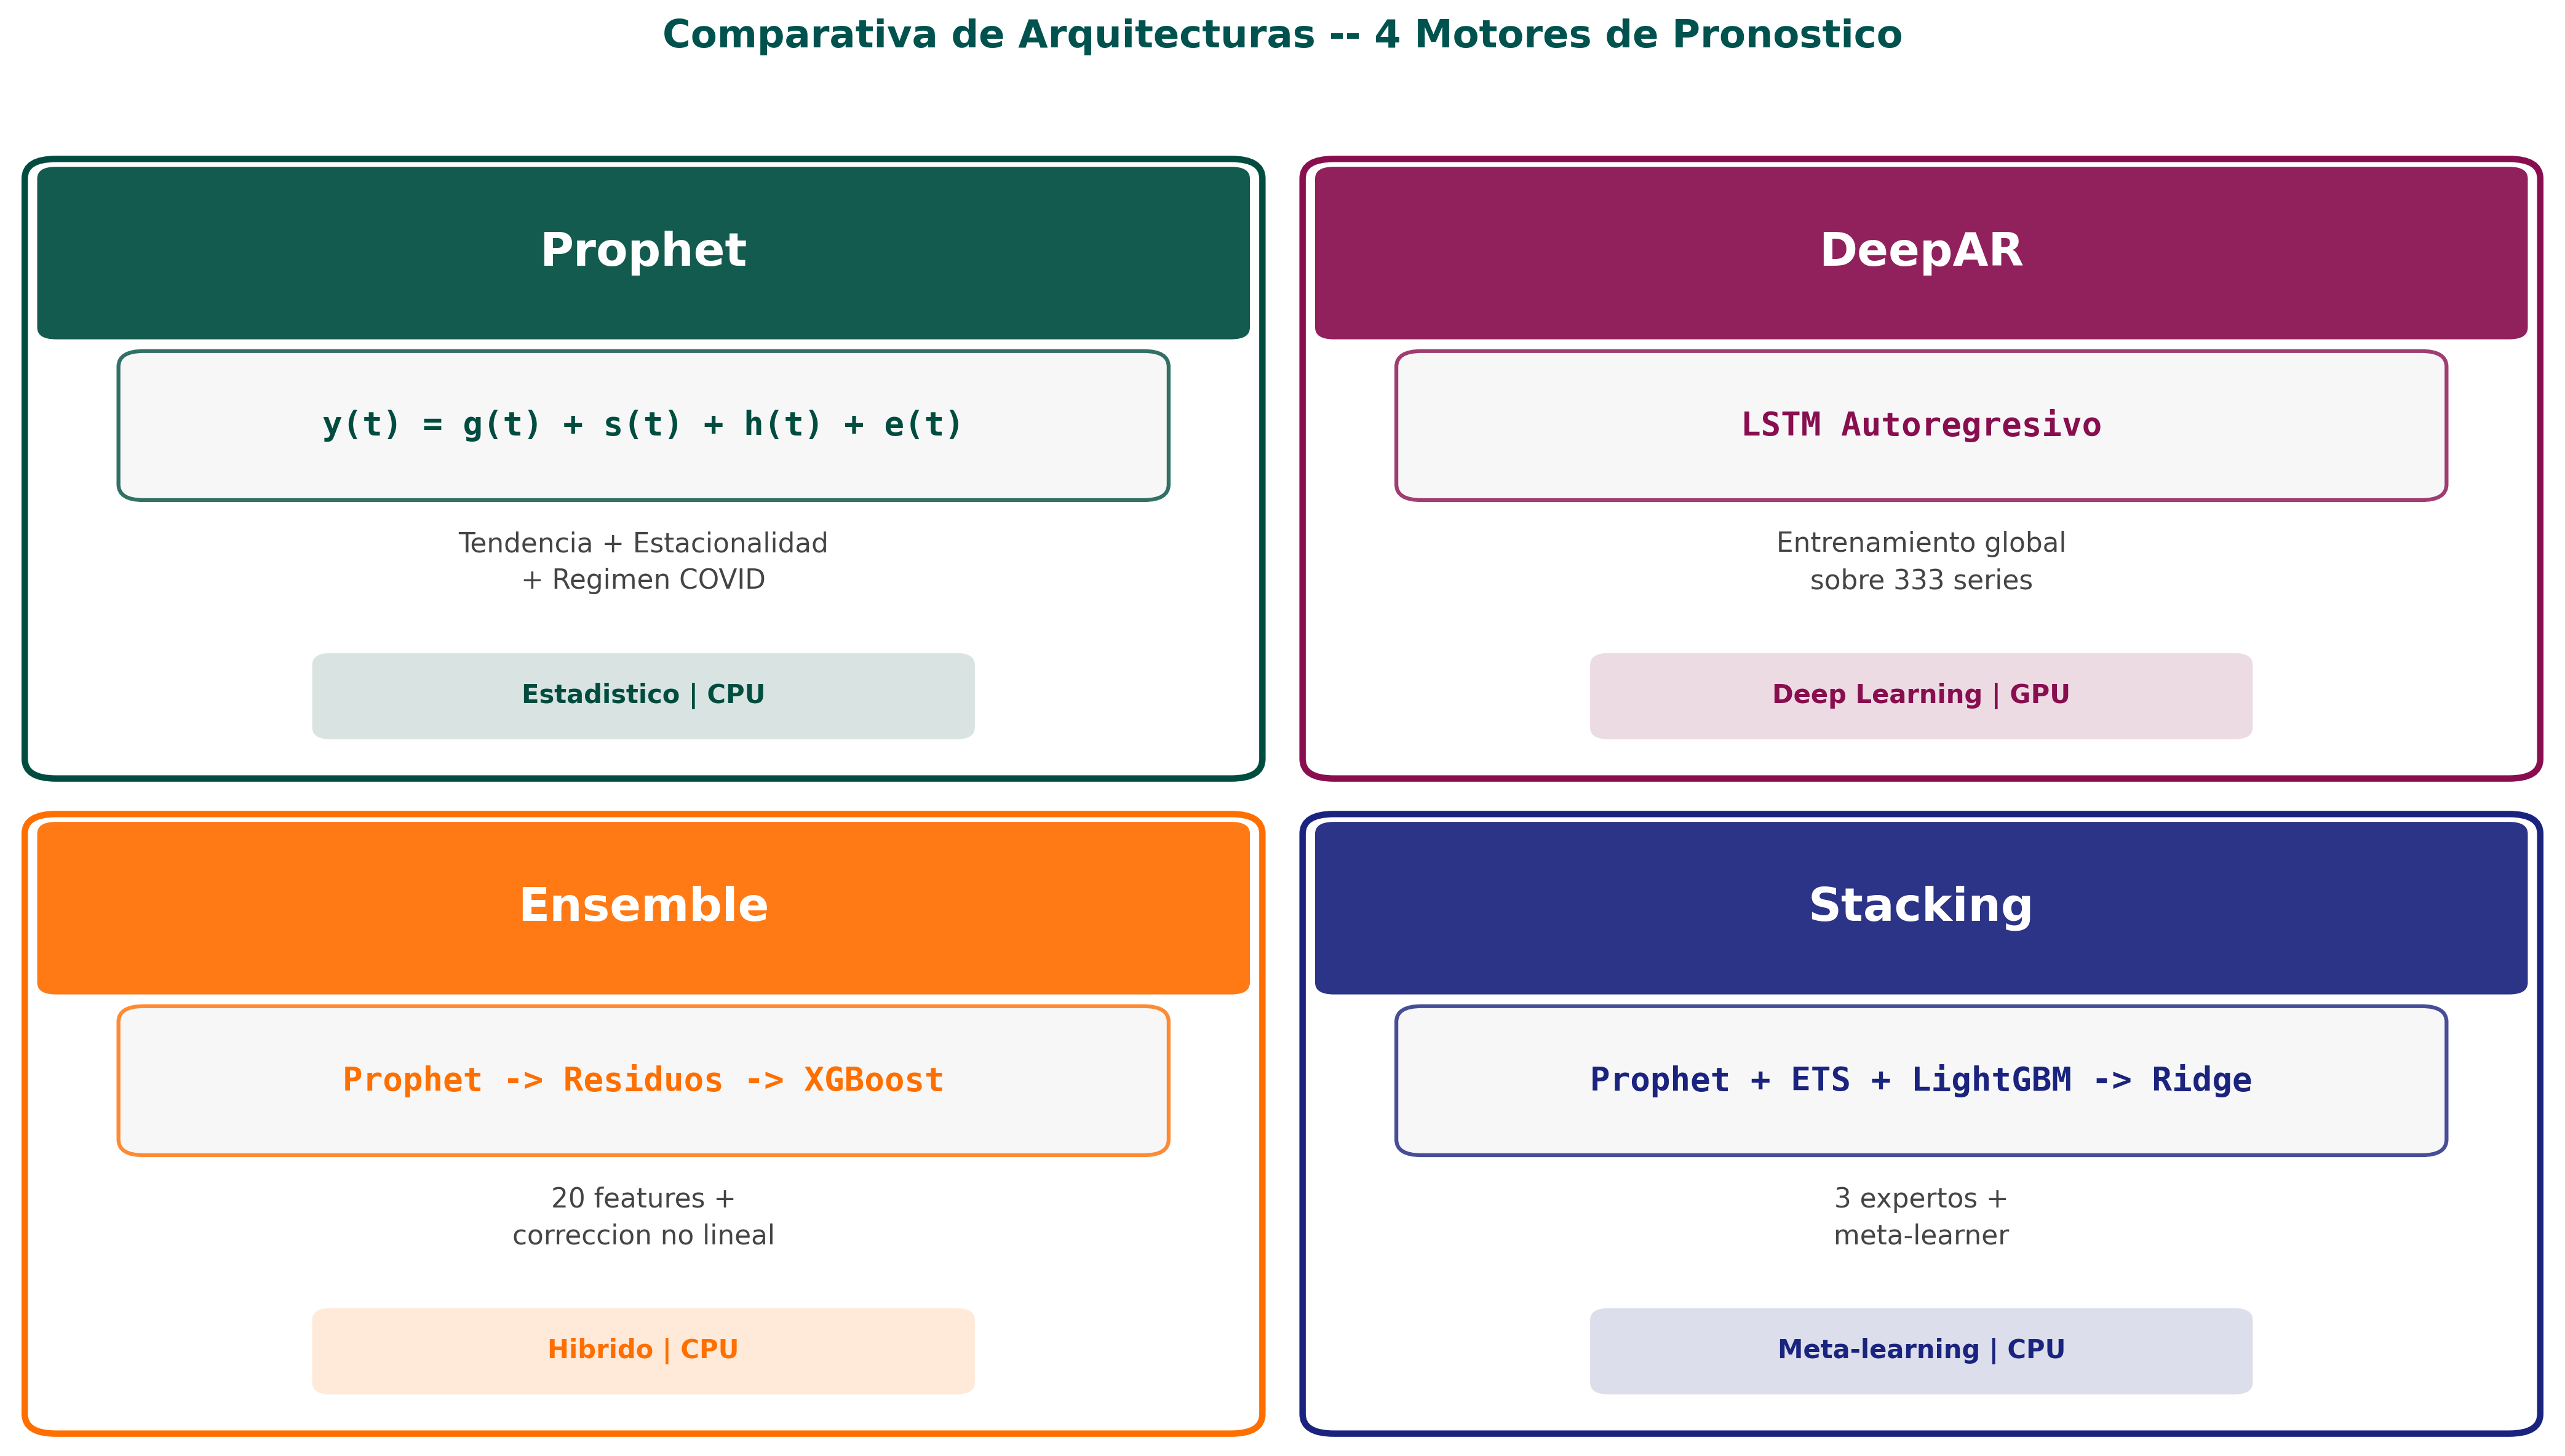
\includegraphics[width=1.05\textwidth]{model_comparison_4panel.png}}
\caption[Comparativa de arquitecturas de los 4 motores.]{Arquitectura de los cuatro motores de pronóstico. Cada motor aborda el problema desde un paradigma distinto: estadístico, deep learning, híbrido y meta-learning.}
\label{fig:model_comparison}
\end{figure}

\subsubsection{Prophet: descomposición aditiva interpretable}

Prophet (Taylor y Letham, 2018) es un modelo de series de tiempo desarrollado por Meta que descompone la señal en componentes aditivos interpretables:
\[
y(t) = g(t) + s(t) + h(t) + \varepsilon_t
\]
donde $g(t)$ es la tendencia (lineal por tramos con detección automática de puntos de cambio), $s(t)$ la estacionalidad (modelada con series de Fourier de orden~10 para el ciclo anual de 365.25~días), $h(t)$ los efectos de régimen (como el periodo COVID-19, mar-2020 a sep-2022) y $\varepsilon_t$ el residuo. En nuestro sistema, Prophet se entrena con 25~changepoints a nivel nacional y 12 a nivel estatal (para evitar sobreajuste en series cortas). La estacionalidad semanal y diaria se desactiva porque los datos tienen granularidad semanal. Prophet destaca en series con estacionalidad fuerte y cambios de régimen conocidos, lo que lo hace especialmente apto para la depresión, que presenta picos estacionales marcados entre febrero y mayo.

\subsubsection{DeepAR: aprendizaje cruzado entre 333~series}

DeepAR (Salinas, Flunkert, Gasthaus y Januschowski, 2020), incorporado por sugerencia de la Dra.~Grettel Barcelo como alternativa de deep learning capaz de aprovechar las 333~series simultáneamente, es una red neuronal recurrente autoregresiva que, a diferencia de los métodos clásicos que ajustan un modelo individual por serie, \textbf{entrena un único modelo global sobre múltiples series simultáneamente}. Esta arquitectura de \textit{cross-learning} permite que el modelo aprenda patrones compartidos entre las 32~entidades (por ejemplo, que la depresión tiene estacionalidad similar en Jalisco y Nuevo León), sin perder la capacidad de capturar particularidades locales.

La red utiliza celdas LSTM con 2--3~capas de 80~unidades cada una, dropout de 0.15, y genera pronósticos probabilísticos muestreando de una distribución Student-t (robusta ante outliers). El contexto de entrada es de 104~semanas (2~años) y el horizonte de predicción de 52~semanas. Se entrena en GPU (NVIDIA T4) vía AWS SageMaker con hasta 300~épocas y early stopping (paciencia de 15~épocas). DeepAR domina en el 73.3\% de las 333~series de producción, confirmando la ventaja del aprendizaje cruzado para datos epidemiológicos de panel.

\subsubsection{Ensemble: corrección de residuos no lineales}\label{sec:ensemble}

El motor Ensemble combina Prophet con XGBoost (Chen y Guestrin, 2016) en una arquitectura de dos etapas:

\begin{enumerate}
  \item \textbf{Primera etapa:} Prophet captura tendencia, estacionalidad y régimen COVID.
  \item \textbf{Segunda etapa:} XGBoost (200~árboles, profundidad~3, learning rate 0.03) recibe las 20~features de la Tabla~\ref{tab:features_catalogo} y aprende a corregir los residuos que Prophet no capturó, incluyendo interacciones no lineales entre lags, momentum y volatilidad.
\end{enumerate}

XGBoost es un sistema de gradient boosting basado en árboles de decisión que ajusta secuencialmente árboles a los residuos del modelo previo, con regularización L1 y L2 para prevenir sobreajuste. A diferencia de la Fase~I, donde XGBoost se utilizó como modelo recursivo autónomo y sufrió acumulación de error, aquí XGBoost \textbf{no} genera predicciones directas de la serie: solo corrige los residuos de Prophet sobre features pre-calculadas, eliminando el problema de la retroalimentación recursiva. La combinación es poderosa porque Prophet aporta la estructura temporal interpretable y XGBoost aporta la capacidad de capturar dinámicas complejas que la descomposición aditiva no modela. El Ensemble entrena 4~folds con ventana expandible (OOF) para calibrar los pesos.

\subsubsection{Stacking: meta-aprendizaje con tres expertos}

El motor Stacking implementa la técnica de \textit{generalización apilada} propuesta por Wolpert (1992) y formalizada por Breiman (1996). Su diseño se inspiró inicialmente en la arquitectura AutoGluon-TimeSeries de Amazon, pero los resultados preliminares con AutoGluon fueron deficientes para nuestras series de baja incidencia, por lo que se desarrolló una implementación propia con tres modelos ``expertos'' que generan predicciones independientes y un meta-learner de segundo nivel que aprende a combinarlas de manera óptima.

\begin{itemize}
  \item \textbf{Experto 1 -- Prophet:} descomposición aditiva (tendencia + estacionalidad Fourier).
  \item \textbf{Experto 2 -- ETS} (Hyndman, Koehler, Snyder y Grose, 2002): suavizamiento exponencial con tendencia y estacionalidad aditivas (periodo de 52~semanas). ETS captura patrones locales de nivel con ponderaciones exponencialmente decrecientes, complementando a Prophet en series con dinámicas más suaves.
  \item \textbf{Experto 3 -- LightGBM} (Ke et al., 2017): gradient boosting con 300~árboles que recibe features trigonométricas ($\sin$, $\cos$ de la semana) y una tendencia lineal. LightGBM utiliza GOSS (muestreo selectivo por gradiente) para acelerar el entrenamiento más de 20$\times$ sin perder precisión.
  \item \textbf{Meta-learner -- Ridge:} regresión Ridge con coeficientes no negativos que aprende los pesos óptimos de cada experto. La restricción de no-negatividad garantiza que las contribuciones sean interpretables y que ningún experto reciba un peso negativo (que equivaldría a ``apostar en contra'' de su predicción).
\end{itemize}

Las predicciones de los expertos se generan mediante validación cruzada out-of-fold (4~folds con ventana expandible), de modo que el meta-learner nunca ve predicciones generadas sobre datos de entrenamiento, evitando sobreajuste.

\subsection{El camino a cuatro motores: experimentación exhaustiva}

La selección de estos cuatro motores no fue arbitraria, sino el resultado de un proceso evolutivo guiado por la retroalimentación de la Dra.~Grettel Barcelo. El punto de partida fue Prophet (heredado de la Fase~I como único motor viable). DeepAR fue incorporado por sugerencia de la asesora como alternativa de deep learning capaz de explotar el aprendizaje cruzado entre series. El motor Ensemble surgió al observar que XGBoost compensaba las debilidades de Prophet en patrones no lineales, pero a diferencia de la Fase~I, como corrector de residuos y no como modelo recursivo. Finalmente, para el Stacking se partió de la arquitectura AutoGluon-TimeSeries de Amazon, pero los resultados iniciales fueron deficientes; se rediseñó con una implementación propia de tres expertos (Prophet, ETS, LightGBM) y un meta-learner Ridge.

En términos de hiperparámetros, el equipo evaluó más de 48~combinaciones solo para Prophet (6~para Alzheimer, 24~para Depresión, 18~para Parkinson), cada una validada en 4~folds temporales con horizonte de 53~semanas. Para DeepAR, se exploraron variantes con 2 y 3~capas LSTM, distribuciones Student-t y Negative-Binomial, y modos single-series vs.\ multi-series (32~estados co-entrenados). La validación cruzada temporal con \textbf{pesos progresivos} (0.5 para el fold más antiguo, 1.25 para el más reciente) refleja que los patrones post-pandemia son más relevantes que los pre-pandemia.

En total, el sistema ejecuta más de \textbf{5,300~entrenamientos individuales} para producir los 333~modelos de producción (333~series $\times$ 4~motores $\times$ 4~folds de validación), un volumen que justifica la infraestructura GPU en AWS SageMaker para DeepAR y el paralelismo con \texttt{joblib} para Prophet.

\subsection{Selección automática del mejor modelo por serie}

Para cada una de las 333~series, el sistema evalúa los cuatro motores mediante validación cruzada con horizonte de 52~semanas (alineado al horizonte de pronóstico real según retroalimentación de la Dra.~Grettel Barcelo, quien señaló que un horizonte de CV menor producía estimaciones demasiado optimistas) y selecciona automáticamente el motor ganador con el siguiente criterio jerárquico:

\begin{enumerate}
  \item \textbf{\smape{}} como métrica primaria (error porcentual simétrico, robusto ante valores cercanos a cero), adoptado por recomendación de la Dra.~Grettel Barcelo en sustitución del MAPE, que se inflaba artificialmente en series de baja incidencia como Alzheimer y Parkinson.
  \item \textbf{\mase{}} como desempate cuando la diferencia de \smape{} es menor al 5\%. El \mase{} compara contra una línea base naive estacional (repetir el valor de hace 52~semanas); un \mase{} < 1 significa que el modelo supera esta referencia.
  \item \textbf{\rmse{}} como segundo desempate.
\end{enumerate}

Series con incidencia extremadamente baja (menos de 5~casos acumulados en 52~semanas) se reasignan al modelo regional correspondiente, garantizando robustez estadística.

\subsection{Lección aprendida: detección y corrección de data leakage}

Durante el desarrollo del motor Ensemble, el equipo detectó un incidente de \textbf{data leakage} (fuga de datos) en las features de ventana deslizante: los valores de la semana actual se incluían como entrada del modelo, lo que inflaba artificialmente las métricas de entrenamiento. La corrección (aplicar un desplazamiento \texttt{shift(1)} para excluir la observación presente) redujo el \smape{} de entrenamiento pero mejoró significativamente la capacidad de generalización del modelo en datos no vistos. Este incidente subraya la importancia de los diagnósticos automatizados de leakage implementados en el sistema (actualmente, 330 de 333~modelos pasan el chequeo) y fue destacado por la Dra.~Grettel Barcelo como un ejemplo de rigurosidad metodológica.

\subsection{Resultados: DeepAR domina}

\begin{figure}[H]
\centering
\makebox[\textwidth][c]{%
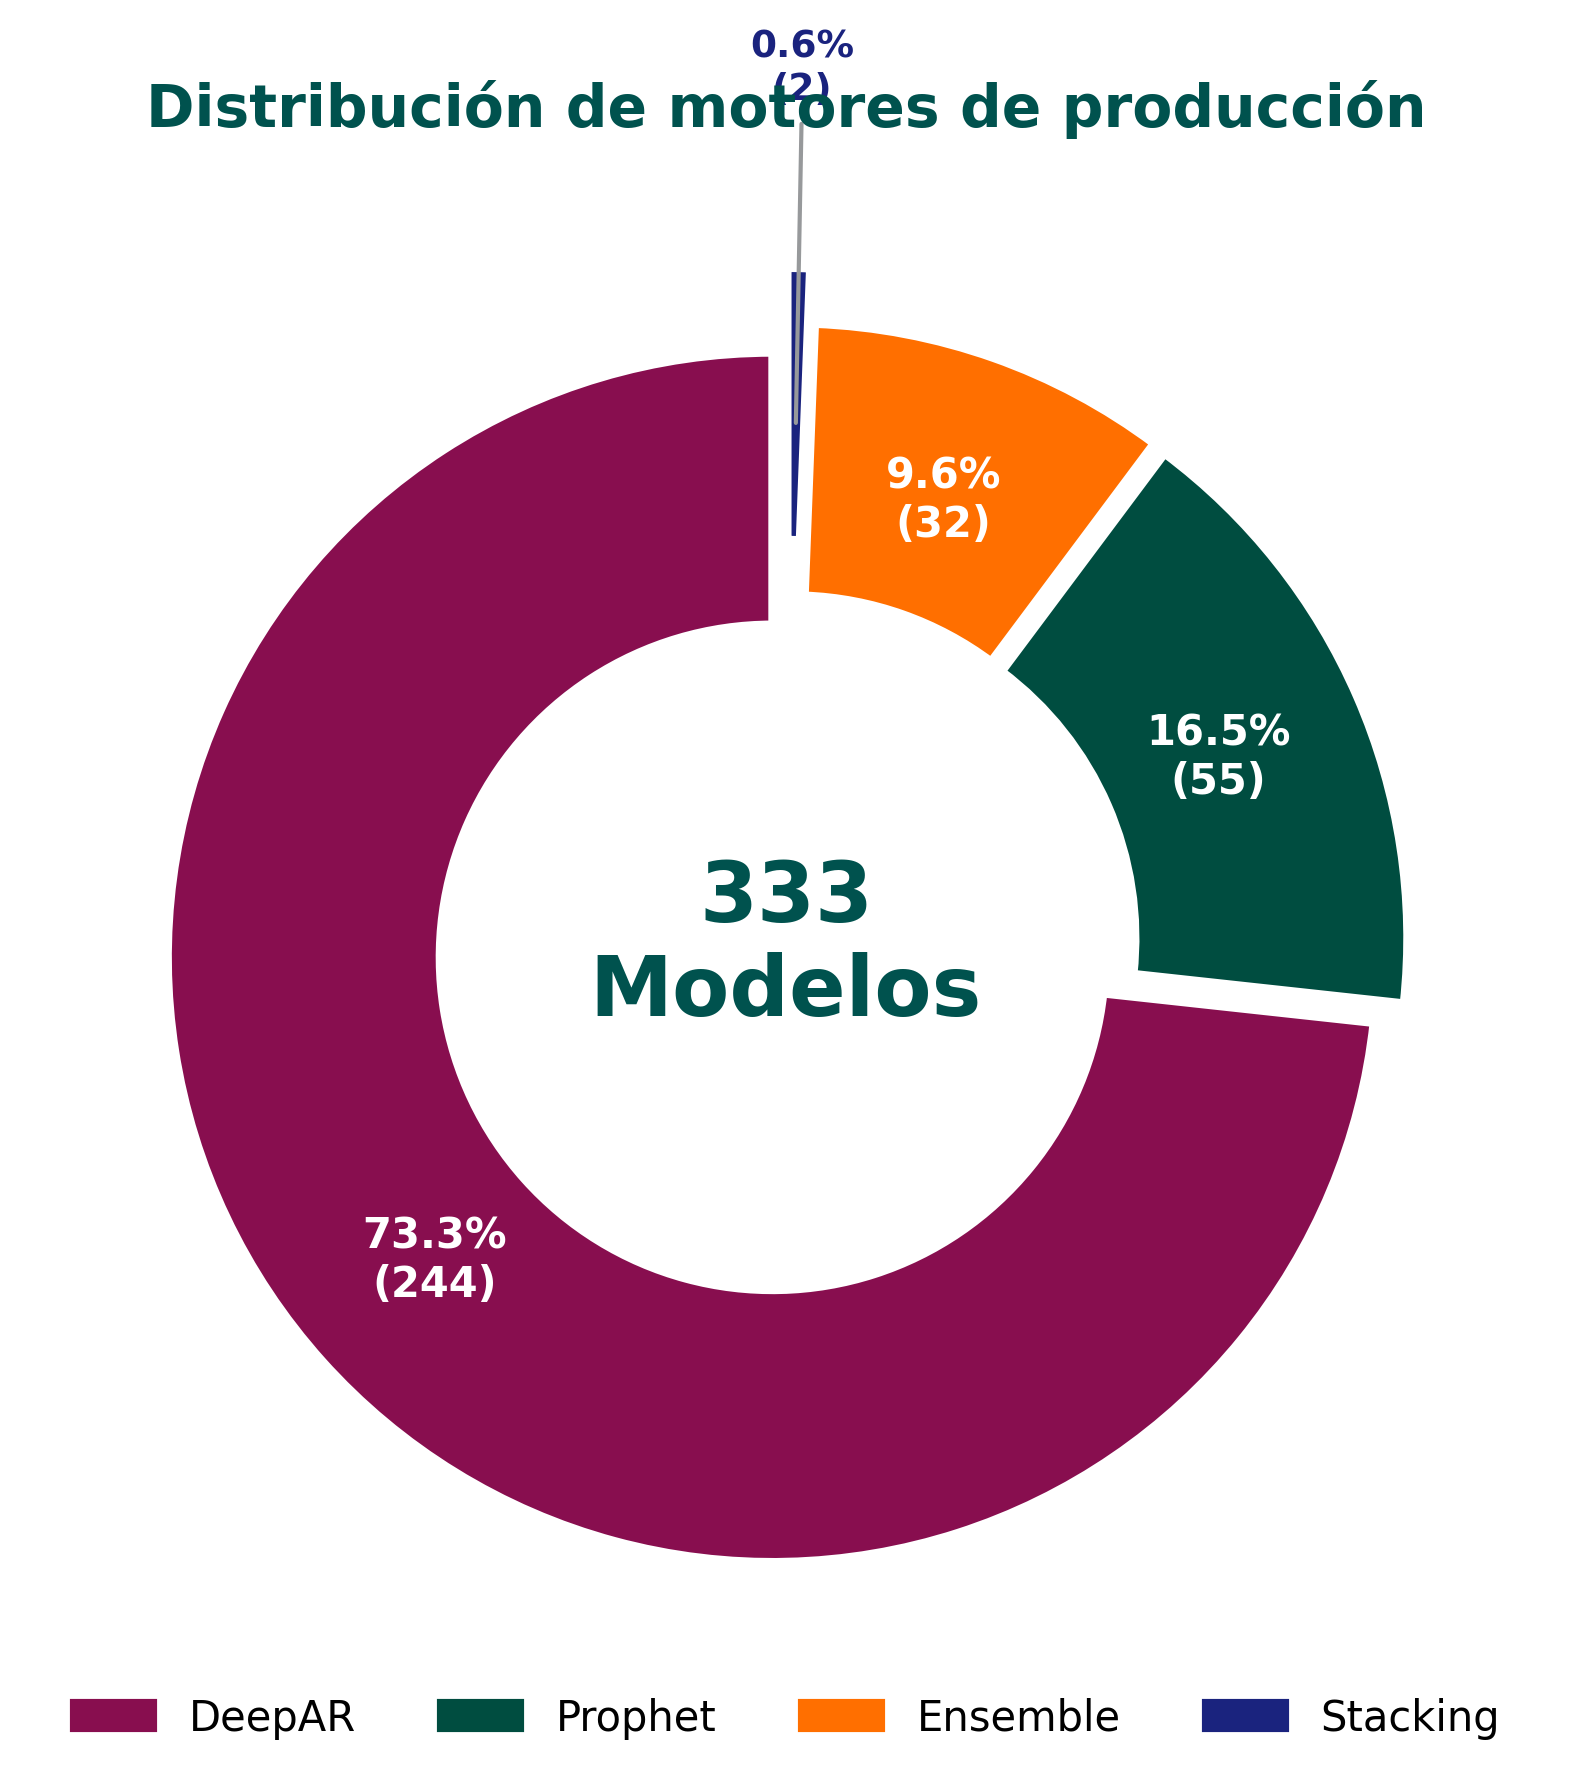
\includegraphics[width=1.0\textwidth]{modelos_distribucion_motores.png}}
\caption[Distribución de motores en producción.]{Distribución de los 333~modelos de producción por motor. DeepAR fue seleccionado como ganador en el 73.3\% de las series, demostrando la ventaja del aprendizaje cruzado entre múltiples series simultáneas.}
\label{fig:distribucion_motores}
\end{figure}

\begin{table}[H]
\centering
\caption{Resumen de rendimiento por motor de pronóstico}
\label{tab:rendimiento_motores}
\small
\begin{tabularx}{\textwidth}{l r r r r r}
\toprule
\textbf{Motor} & \textbf{Series} & \textbf{\%} & \textbf{\smape{} med.} & \textbf{\mase{} med.} & \textbf{MASE < 1} \\
\midrule
DeepAR    & 244 & 73.3\% & 11.68\% & 0.20 & 97.5\% \\
Prophet   &  55 & 16.5\% & 136.63\% & 0.77 & 96.4\% \\
Ensemble  &  32 &  9.6\% & 141.58\% & 0.84 & 71.9\% \\
Stacking\textsuperscript{$\dagger$}  &   2 &  0.6\% & 33.05\% & 0.54 & 100.0\% \\
\midrule
\textbf{Global} & \textbf{333} & \textbf{100\%} & \textbf{23.66\%} & \textbf{0.30} & \textbf{94.9\%} \\
\bottomrule
\end{tabularx}
\begin{flushleft}
\scriptsize \textsuperscript{$\dagger$} Muestra limitada (2~series). Los valores altos de \smape{} en Prophet y Ensemble reflejan que estos motores ganan en series de baja incidencia donde el \smape{} se infla; su \mase{} confirma que aun así superan la línea base naive.
\end{flushleft}
\end{table}

\begin{insightbox}
\textbf{Hallazgo clave:} El 94.9\% de los 333~modelos de producción superan la línea base naive estacional (\mase{} < 1). Esto significa que el sistema de pronóstico es, en la gran mayoría de los casos, \textbf{más preciso que simplemente repetir lo que ocurrió el año anterior}. La mediana global de \mase{} de 0.30 indica que el error típico del sistema es un 70\% menor que el de la referencia naive.
\end{insightbox}

\begin{figure}[H]
\centering
\makebox[\textwidth][c]{%
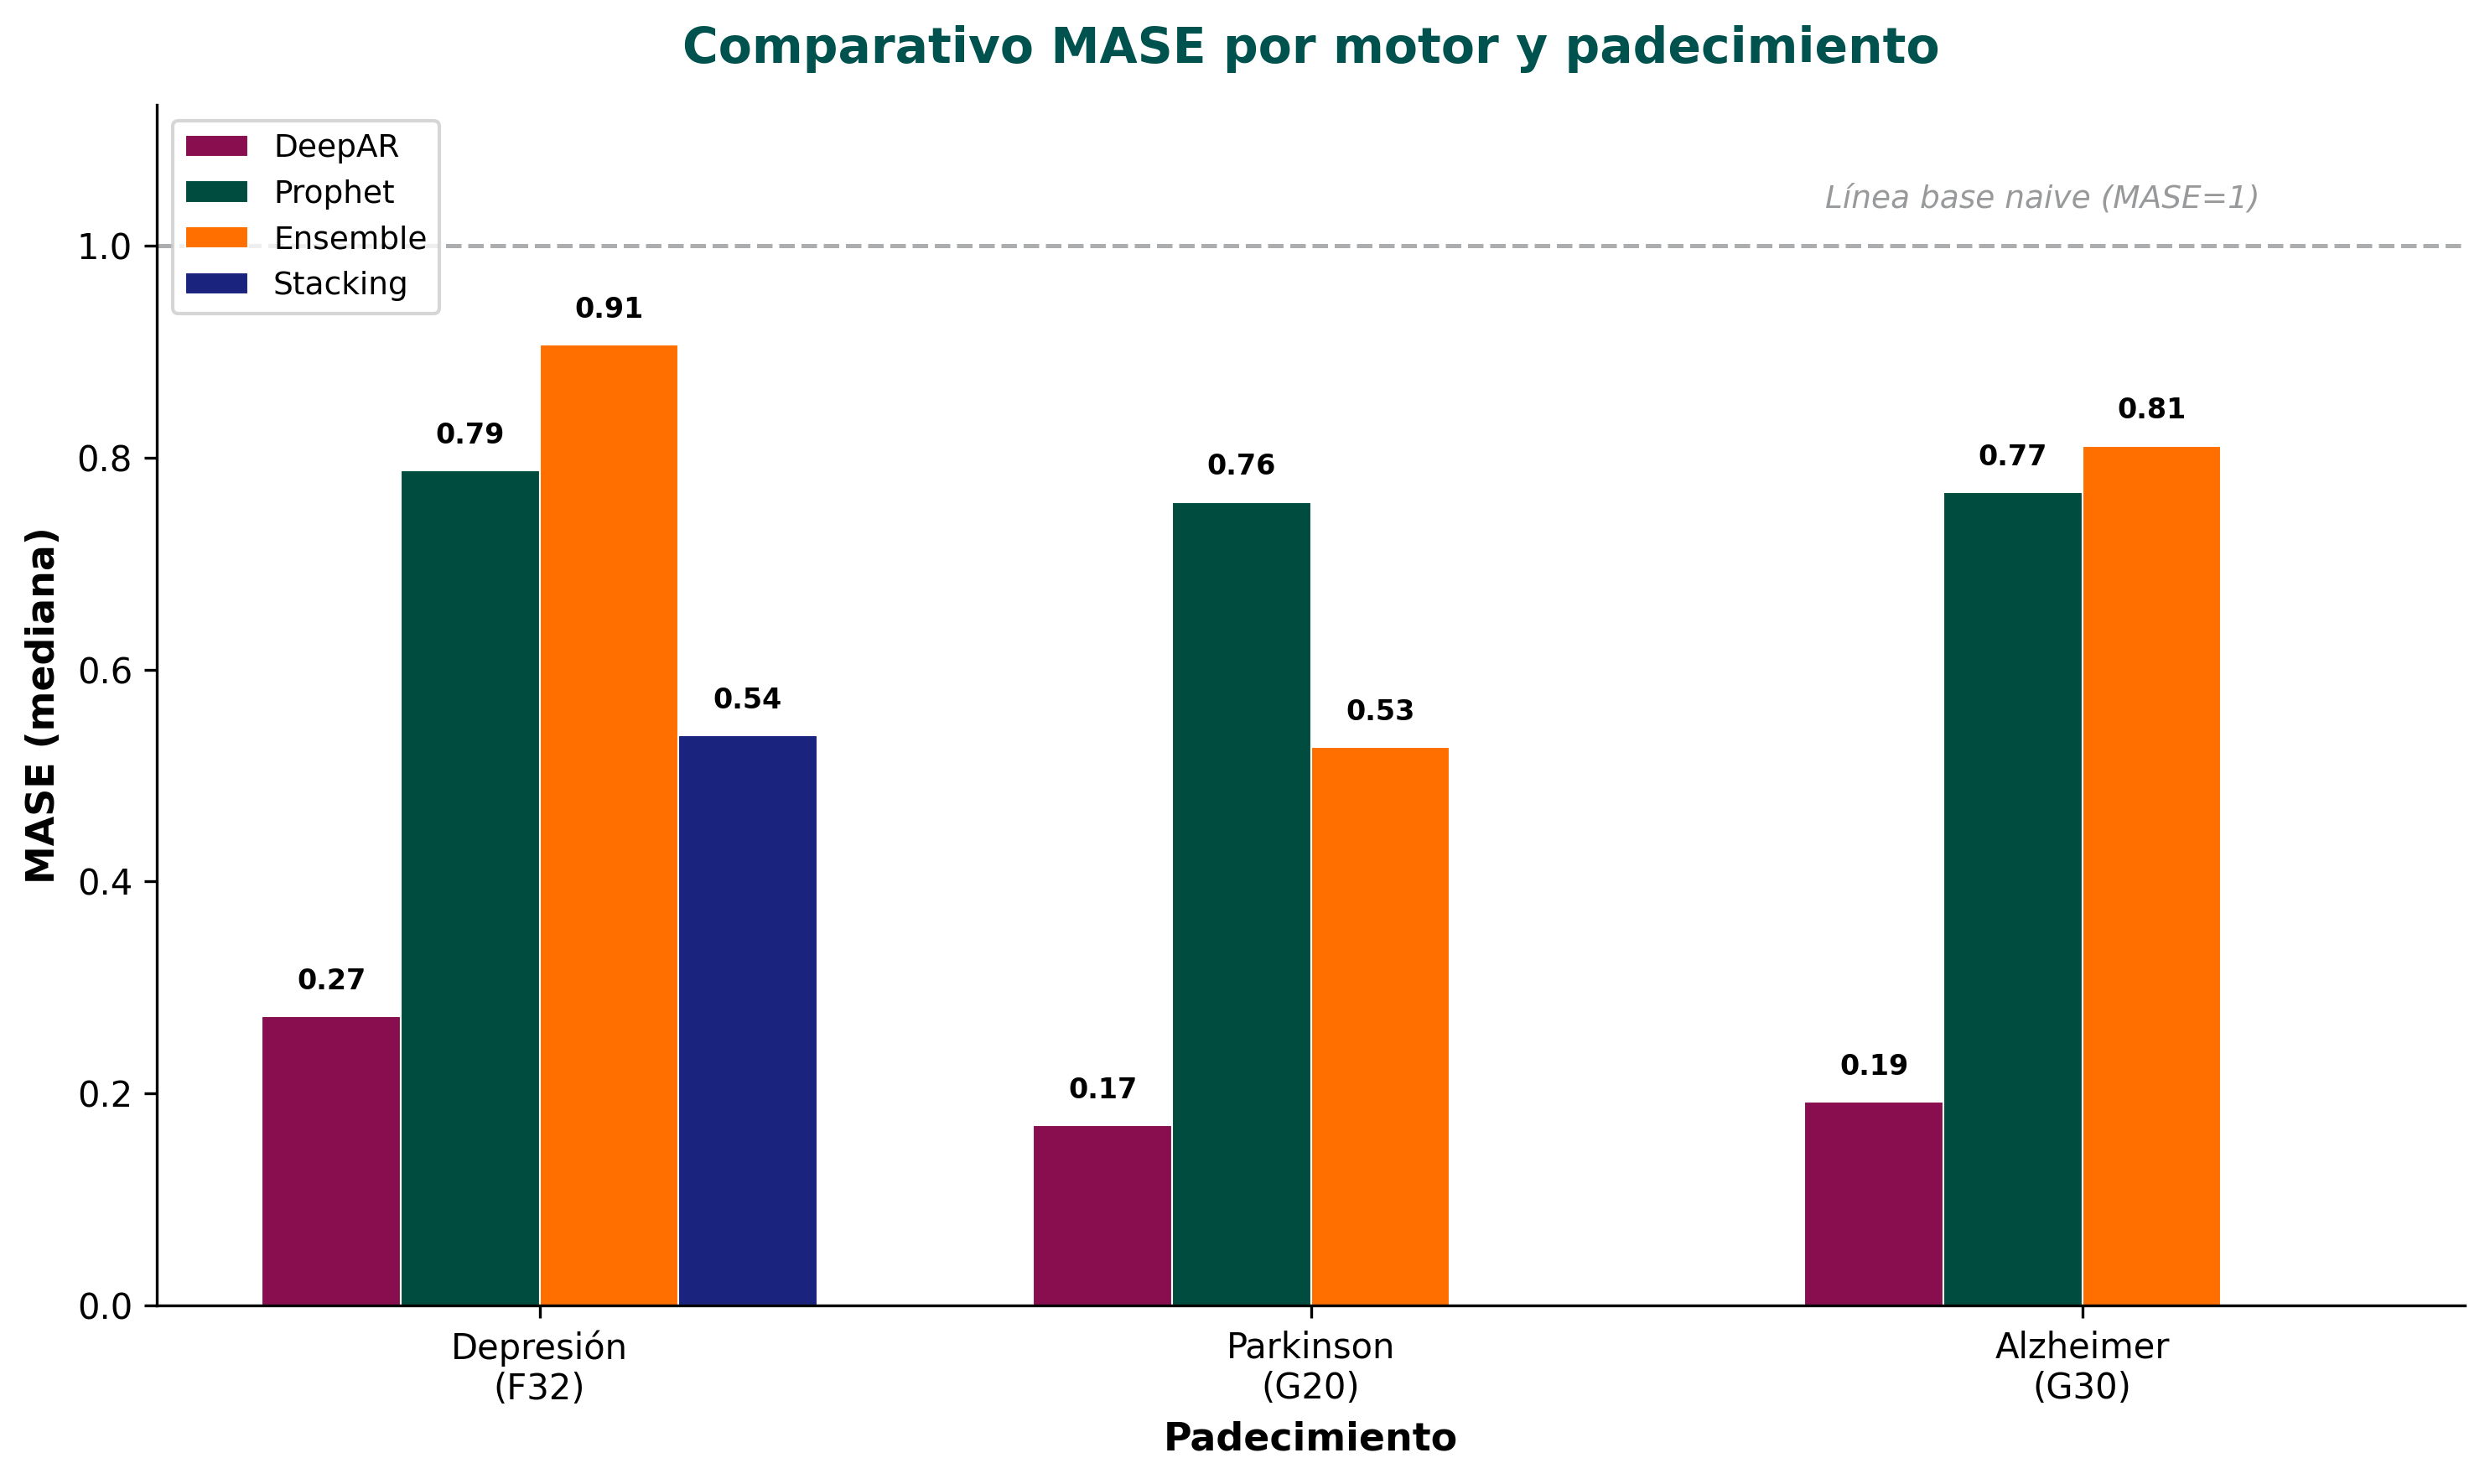
\includegraphics[width=1.15\textwidth]{modelos_comparativo_mase.png}}
\caption[Comparativo de MASE por motor y padecimiento.]{Comparación de \mase{} mediana por motor y padecimiento. La línea punteada en \mase{} = 1.0 marca el umbral de la línea base naive: valores por debajo indican que el modelo supera la referencia.}
\label{fig:comparativo_mase}
\end{figure}

\subsection{Rendimiento por padecimiento}

\begin{table}[H]
\centering
\caption{Métricas de producción por padecimiento}
\label{tab:metricas_padecimiento}
\small
\begin{tabularx}{\textwidth}{l r r r r r}
\toprule
\textbf{Padecimiento} & \textbf{Series} & \textbf{\smape{} med.} & \textbf{\mase{} med.} & \textbf{Casos 52 sem.} & \textbf{\mase{} < 1} \\
\midrule
Depresión (F32)  & 111 &  5.99\% & 0.17 & 155,966 & 100.0\% \\
Parkinson (G20)  & 111 & 35.24\% & 0.26 &   8,234 &  94.6\% \\
Alzheimer (G30)  & 111 & 107.59\% & 0.63 &   1,249 &  90.1\% \\
\midrule
\textbf{Global}  & \textbf{333} & \textbf{23.66\%} & \textbf{0.30} & \textbf{165,449} & \textbf{94.9\%} \\
\bottomrule
\end{tabularx}
\end{table}

\begin{warningbox}
\textbf{Nota sobre Alzheimer:} El \smape{} mediano de 107.59\% no indica un modelo deficiente, sino un \textbf{artefacto matemático} de la baja incidencia. Cuando la realidad es 1--2 casos por semana y el pronóstico es 2--3 casos, el \smape{} se dispara aunque el error absoluto sea menor a un caso. La métrica \mase{} (0.63) confirma que incluso para Alzheimer, el modelo supera la línea base naive.
\end{warningbox}

Con 333~modelos en producción y métricas que superan la línea base naive en el 94.9\% de las series, el siguiente desafío es hacer que esta inteligencia epidemiológica llegue a quien la necesita. Las siguientes tres secciones presentan el ecosistema de herramientas diseñado para tres audiencias distintas: directivos, equipo técnico y personal clínico.

% ============================================================
% 5. SHOWCASE: EPIDASHBOARD (TABLEAU)
% ============================================================
\newpage
\section{Centro de Inteligencia Epidemiológica: EpiDashboard}\label{sec:dashboard}

El EpiDashboard es la interfaz de visualización que transforma los pronósticos de las 333~series en información \textbf{accionable} para los tomadores de decisiones del \imss{}. Desarrollado por Luis Gerardo Sanchez Salazar, este dashboard interactivo está disponible en producción en \url{https://proyectointegrador.org/epidashboard}.

\subsection{Propósito y público objetivo}

El dashboard está diseñado para tres audiencias:

\begin{itemize}
  \item \textbf{Directivos \imss{}:} visión nacional con indicadores clave de desempeño (KPIs), semáforos de alerta y tendencias a 52~semanas.
  \item \textbf{Coordinadores estatales:} filtrado por entidad federativa, padecimiento y género para planificación operativa local.
  \item \textbf{Equipos de planificación:} comparación histórica vs.~predicción, identificación de estados críticos y distribución de recursos.
\end{itemize}

\subsection{Capacidades principales}

El sistema de visualización comprende 20~vistas en 4~dashboards temáticos:

\begin{enumerate}
  \item \textbf{Dashboard Nacional:} acumulado de casos por año, tendencias históricas, comparación entre padecimientos.
  \item \textbf{Dashboard Regional:} incidencia por región de salud mental (4~regiones + nacional), normalización por 100,000~habitantes.
  \item \textbf{Dashboard de Desempeño:} métricas de precisión por modelo, semáforos de confianza, selección automática del modelo productivo.
  \item \textbf{Dashboard de KPIs:} 333~series con indicadores de \smape{}, \mase{}, distribución de motores y diagnósticos de calidad.
\end{enumerate}

\begin{figure}[H]
\centering
\begin{subfigure}[b]{\textwidth}
\centering
\makebox[\textwidth][c]{%
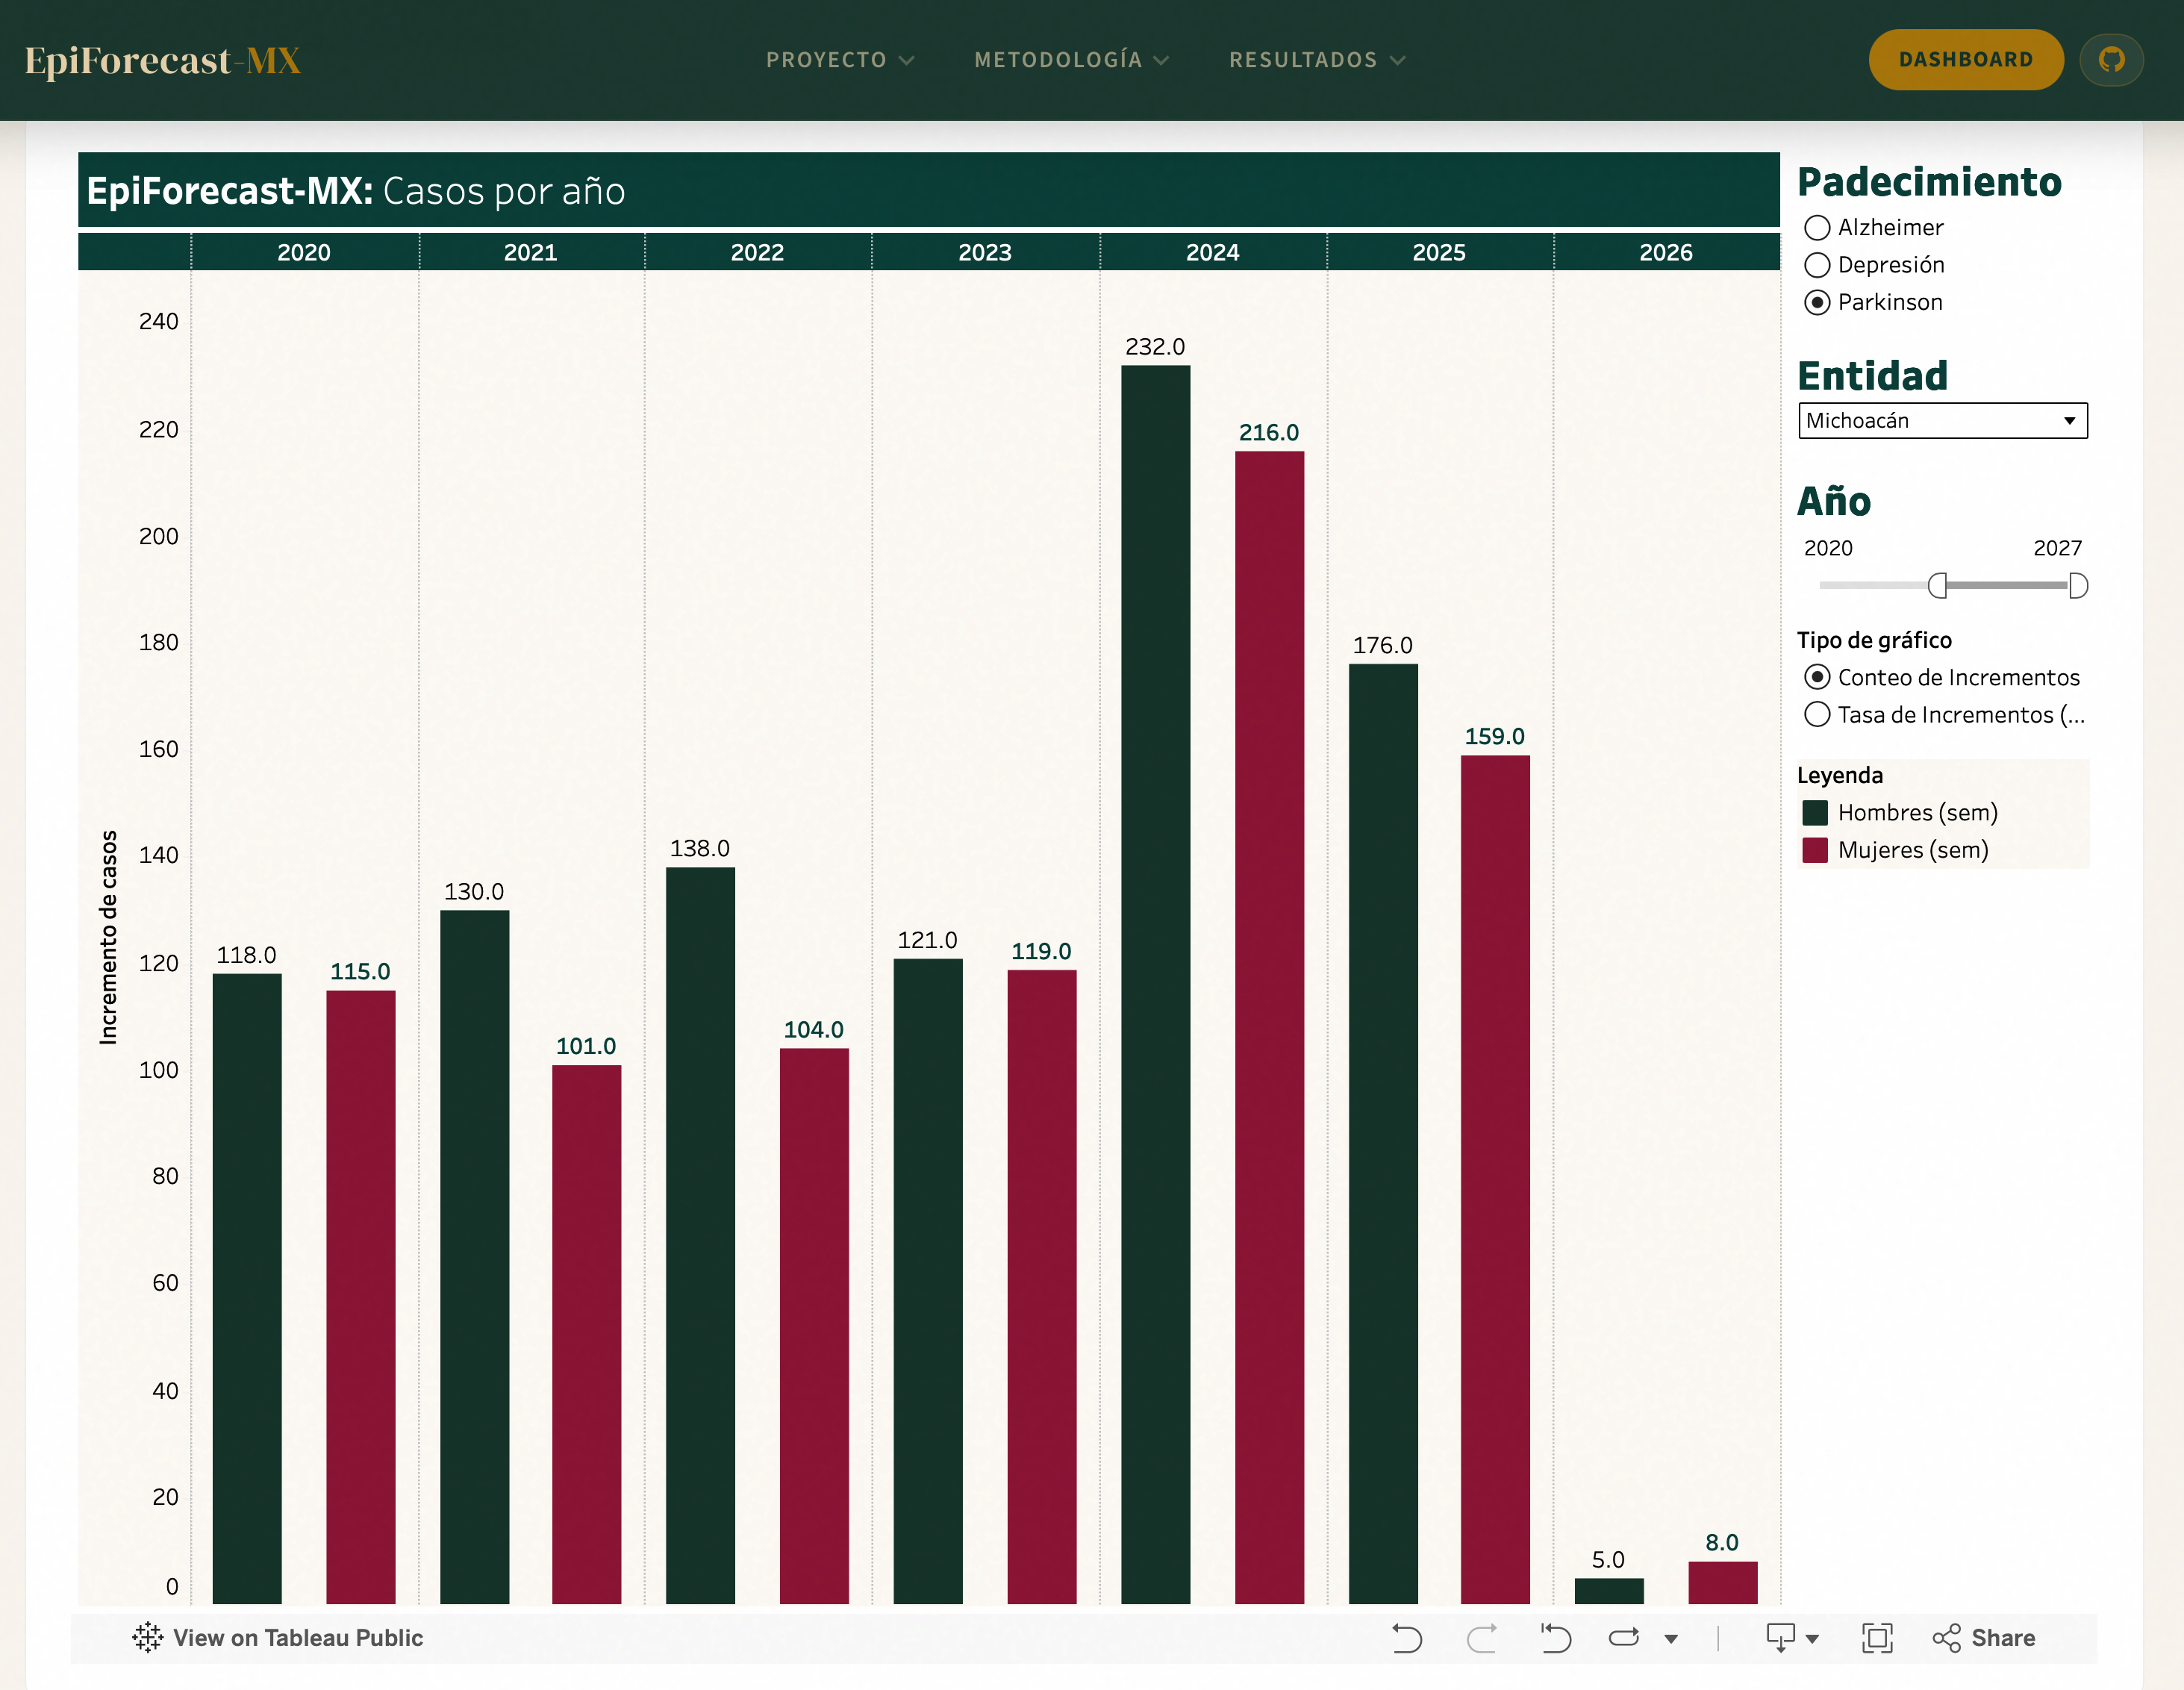
\includegraphics[width=1.15\textwidth]{dashboard_nacional.png}}
\caption{Dashboard Nacional: acumulado de casos por año y tendencias históricas.}
\label{fig:dashboard_nacional}
\end{subfigure}

\vspace{0.4cm}

\begin{subfigure}[b]{\textwidth}
\centering
\makebox[\textwidth][c]{%
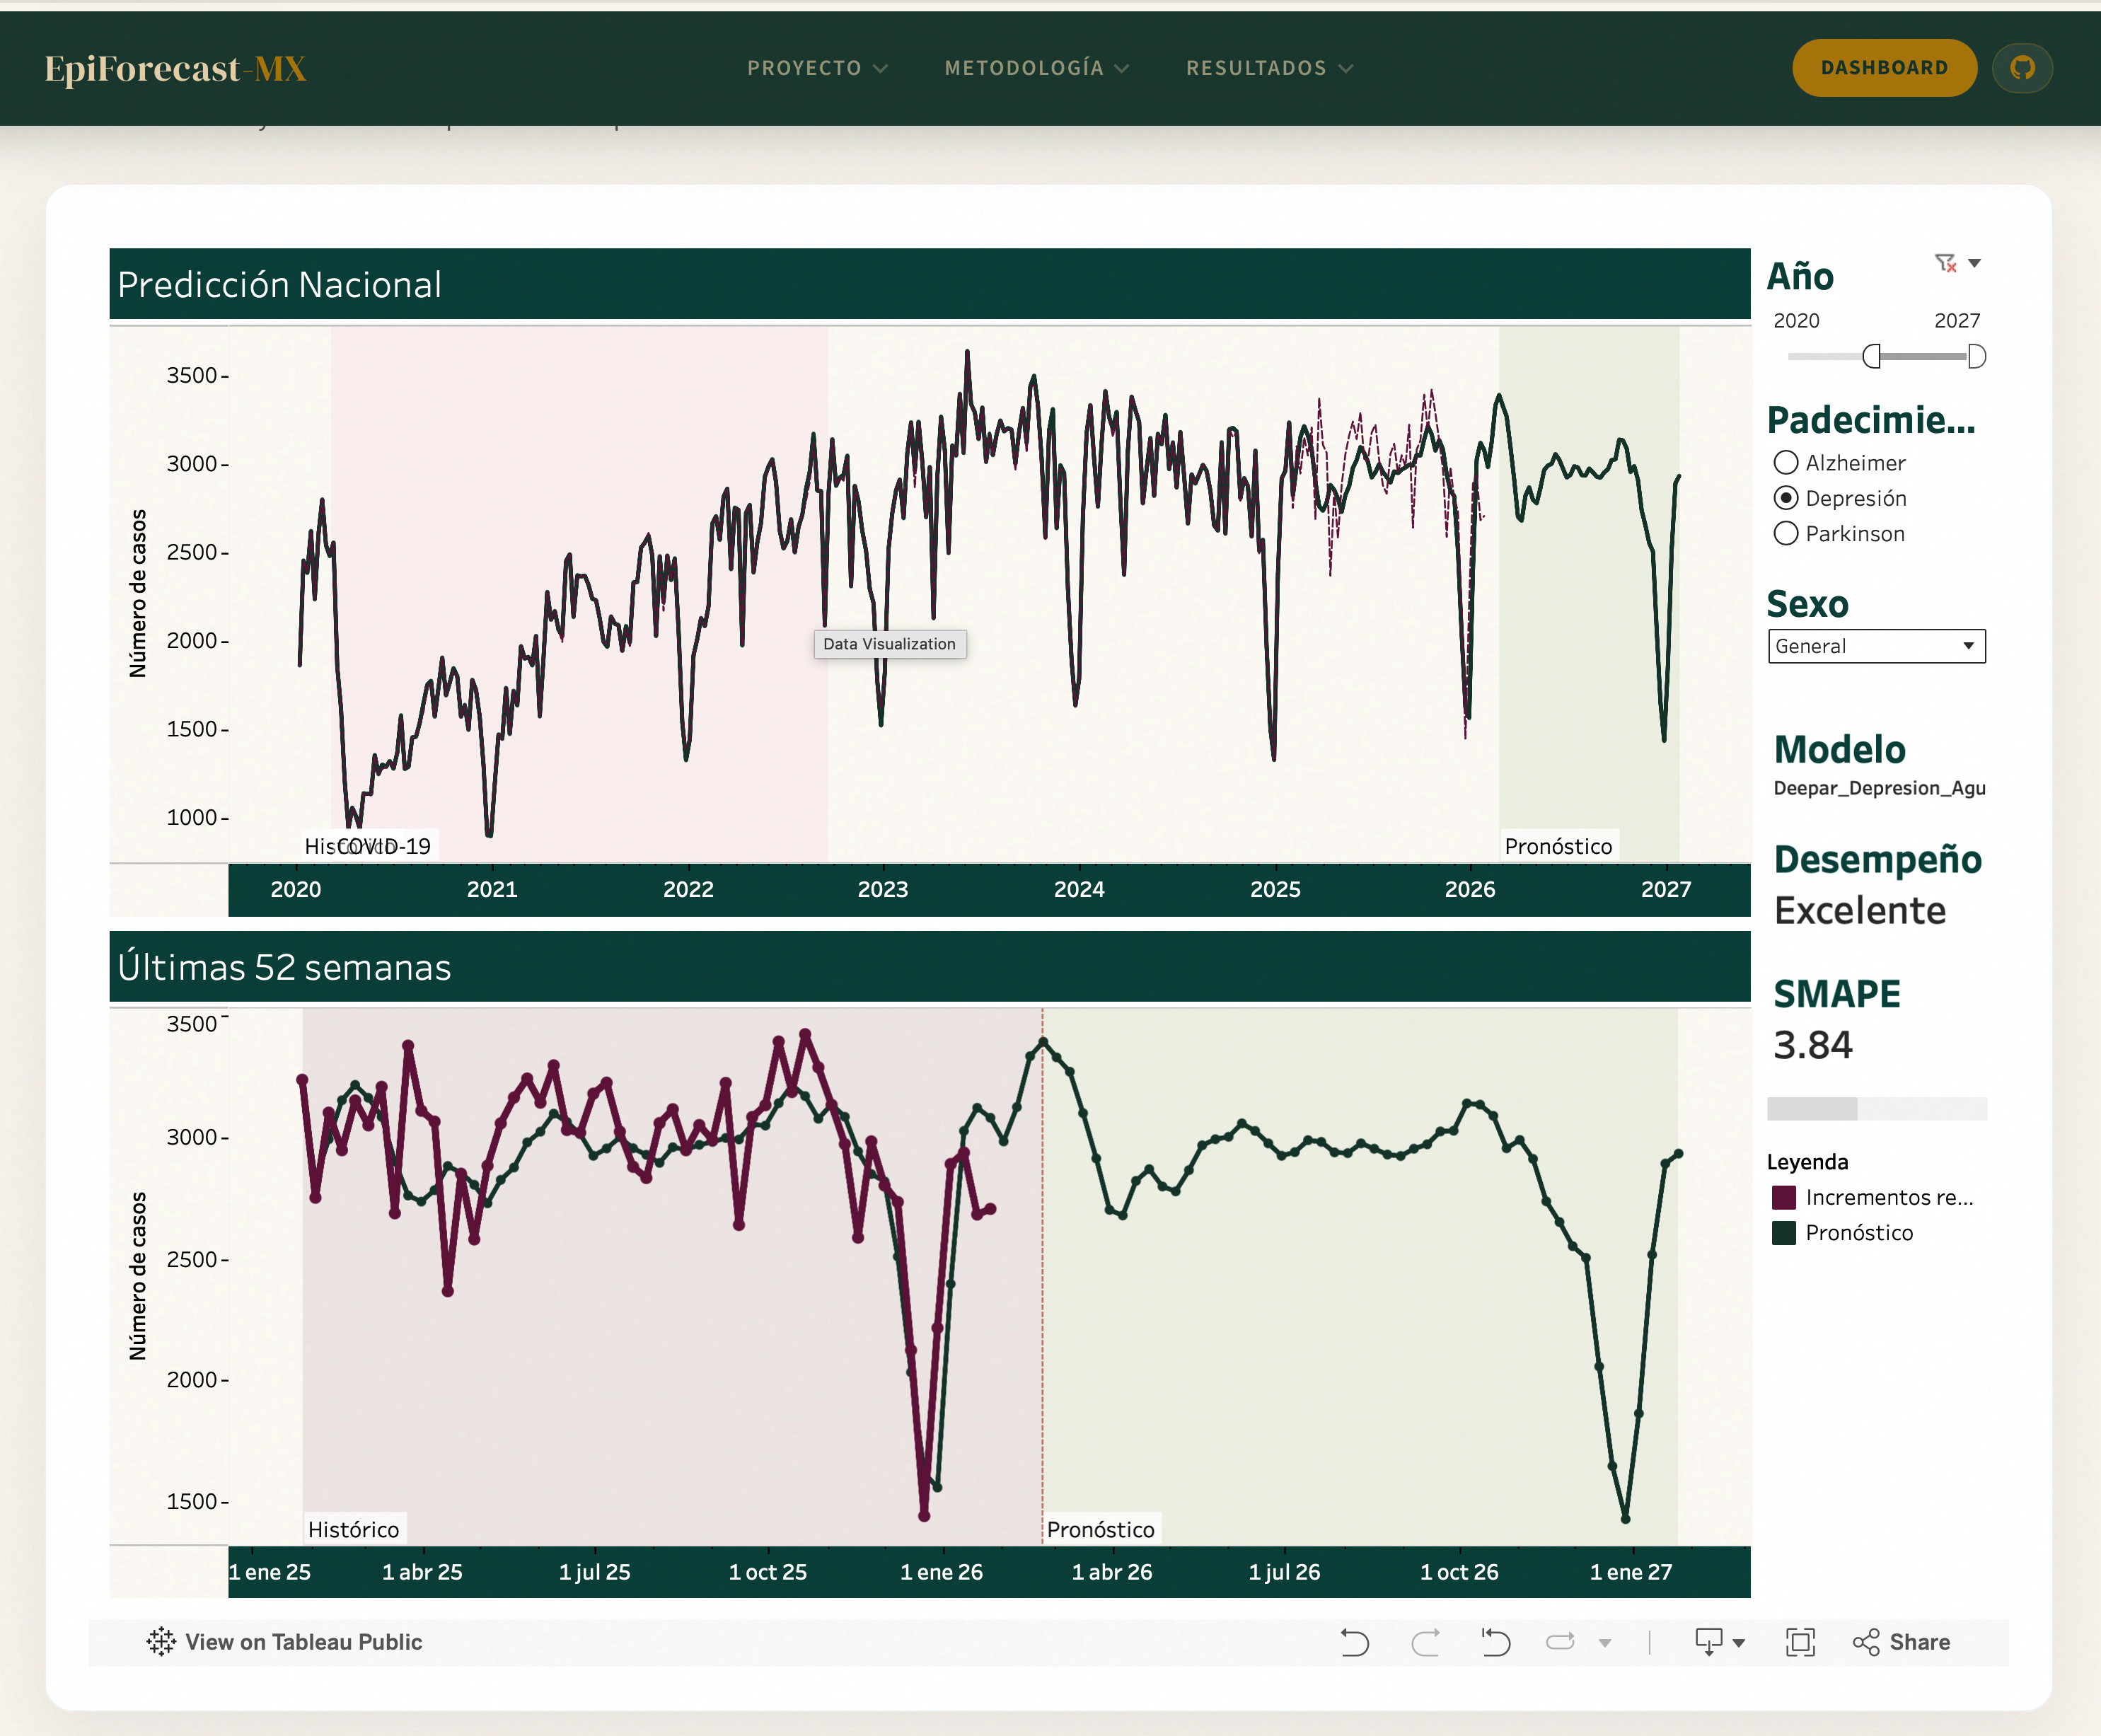
\includegraphics[width=1.15\textwidth]{dashboard_prediccion.png}}
\caption{Dashboard de Predicción: zoom a 52~semanas previas y futuras con bandas de confianza.}
\label{fig:dashboard_prediccion}
\end{subfigure}
\caption[EpiDashboard Tableau en producción.]{EpiDashboard Tableau en producción: (a)~vista nacional con acumulado de casos por año y (b)~vista de predicción con horizonte de 52~semanas. El dashboard ofrece 20~vistas en 4~paneles temáticos.}
\label{fig:dashboard_showcase}
\end{figure}

\begin{figure}[H]
\centering
\makebox[\textwidth][c]{%
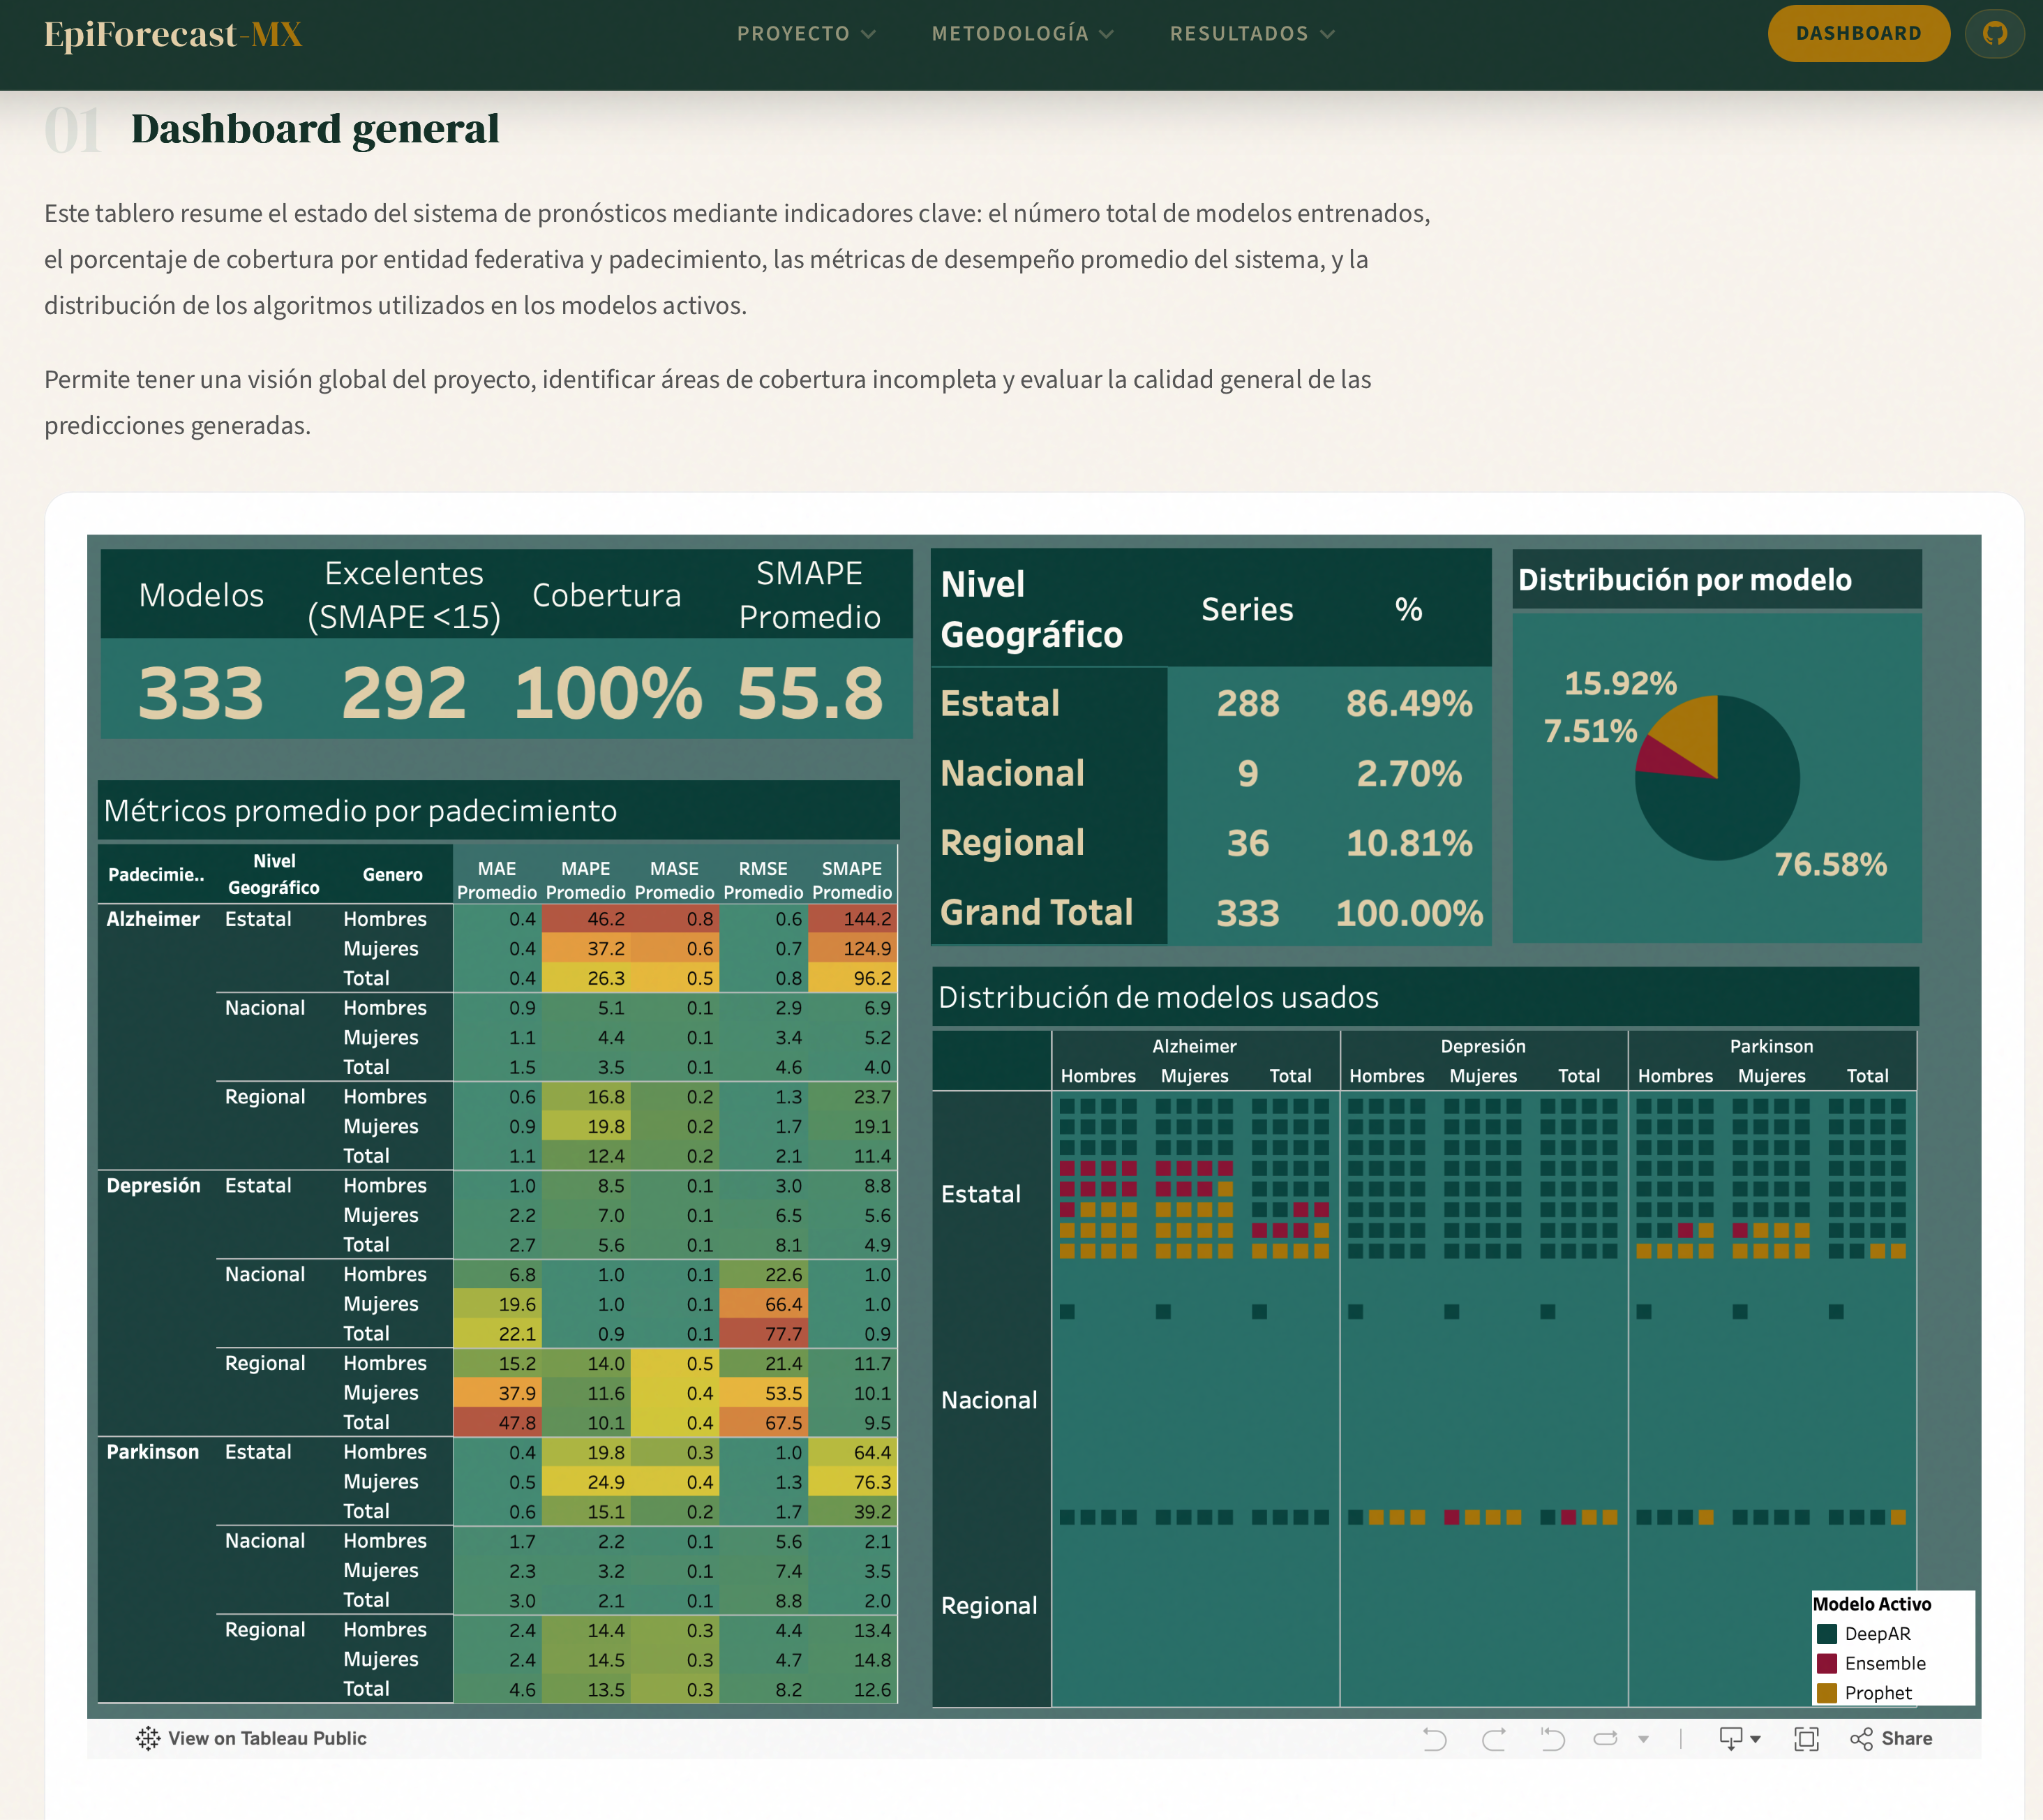
\includegraphics[width=1.15\textwidth]{dashboard_showcase.png}}
\caption[EpiDashboard -- Panel de KPIs y modelos.]{Panel de KPIs mostrando los 333~modelos de producción con métricas de rendimiento, distribución de motores ganadores y semáforos de calidad.}
\label{fig:dashboard_kpis}
\end{figure}

\subsection{Arquitectura del flujo de datos}

El pipeline de datos que alimenta el dashboard opera de manera automatizada:

\begin{center}
\small
\texttt{build\_tableau.py} $\rightarrow$ \texttt{GitHub Actions} $\rightarrow$ \texttt{Google Sheets} $\rightarrow$ \texttt{Tableau Public} $\rightarrow$ \texttt{proyectointegrador.org}
\end{center}

Este flujo garantiza que el dashboard se actualice automáticamente cada vez que se ejecuta el pipeline de inferencia, sin intervención manual. La arquitectura relacional del dataset, compuesta por 5~tablas normalizadas, redujo el volumen de datos en un 84.9\% respecto al diseño original de tabla plana, optimizando el rendimiento de Tableau Public.

% ============================================================
% 6. SHOWCASE: EPI CONSOLA
% ============================================================
\newpage
\section{EPI Consola: Centro de Comando para el Equipo Técnico}\label{sec:consola}

La EPI Consola es la interfaz de línea de comandos (CLI) diseñada para que el equipo técnico del \imss{} opere el sistema de pronóstico sin necesidad de memorizar decenas de comandos de AWS, DVC y Git. Es, en esencia, un \textbf{centro de comando unificado} con branding institucional.

\subsection{El problema que resuelve}

Operar un sistema MLOps completo implica coordinar múltiples herramientas: SageMaker para entrenamiento GPU, DVC para versionado de datos, S3 para almacenamiento, GitHub Actions para CI/CD, y más de 55~targets del Makefile para orquestar el pipeline. Sin la EPI Consola, un operador necesitaría recordar y combinar manualmente estos comandos:

\begin{criticalbox}
\textbf{Sin EPI Consola:}\\
\texttt{python -m scripts.entrena modelo\_activo='deepar' padecimiento.tipo='Depresion'}\\
\texttt{dvc push models/deepar/Depresion/}\\
\texttt{python -m scripts.predice modelo\_activo='deepar'}\\
\texttt{aws s3 sync reports/forecasts/ s3://epiforecast-mx-data/forecasts/}\\[0.3cm]
\textbf{Con EPI Consola:}\\
\texttt{> entrena deepar depresión}\\
\texttt{> sincroniza modelos}
\end{criticalbox}

\subsection{Capacidades principales}

\begin{itemize}
  \item \textbf{NLP en español:} clasificador de intenciones con 17+~categorías que traduce lenguaje natural a comandos del pipeline. El operador puede escribir \texttt{``muestra los modelos de parkinson''} y el sistema interpreta la intención correcta.
  \item \textbf{Dashboard interactivo:} panel multi-sección con datos en tiempo real del boletín epidemiológico, inventario de modelos, métricas de pronóstico y estadísticas de sesión.
  \item \textbf{Navegador de modelos:} tabla paginada de los 333~modelos con \smape{} codificado por colores y badges de diagnóstico (overfitting, leakage).
  \item \textbf{Visor de pronósticos:} sparklines de pronósticos a 52~semanas con tendencia visual.
  \item \textbf{Clasificación de riesgo:} cada comando se clasifica como seguro, modificador o destructivo, con gates de aprobación para operaciones críticas.
  \item \textbf{Chat IA integrado:} base de conocimiento local del proyecto con fallback a Gemini para consultas abiertas.
\end{itemize}

\begin{figure}[H]
\centering
\makebox[\textwidth][c]{%
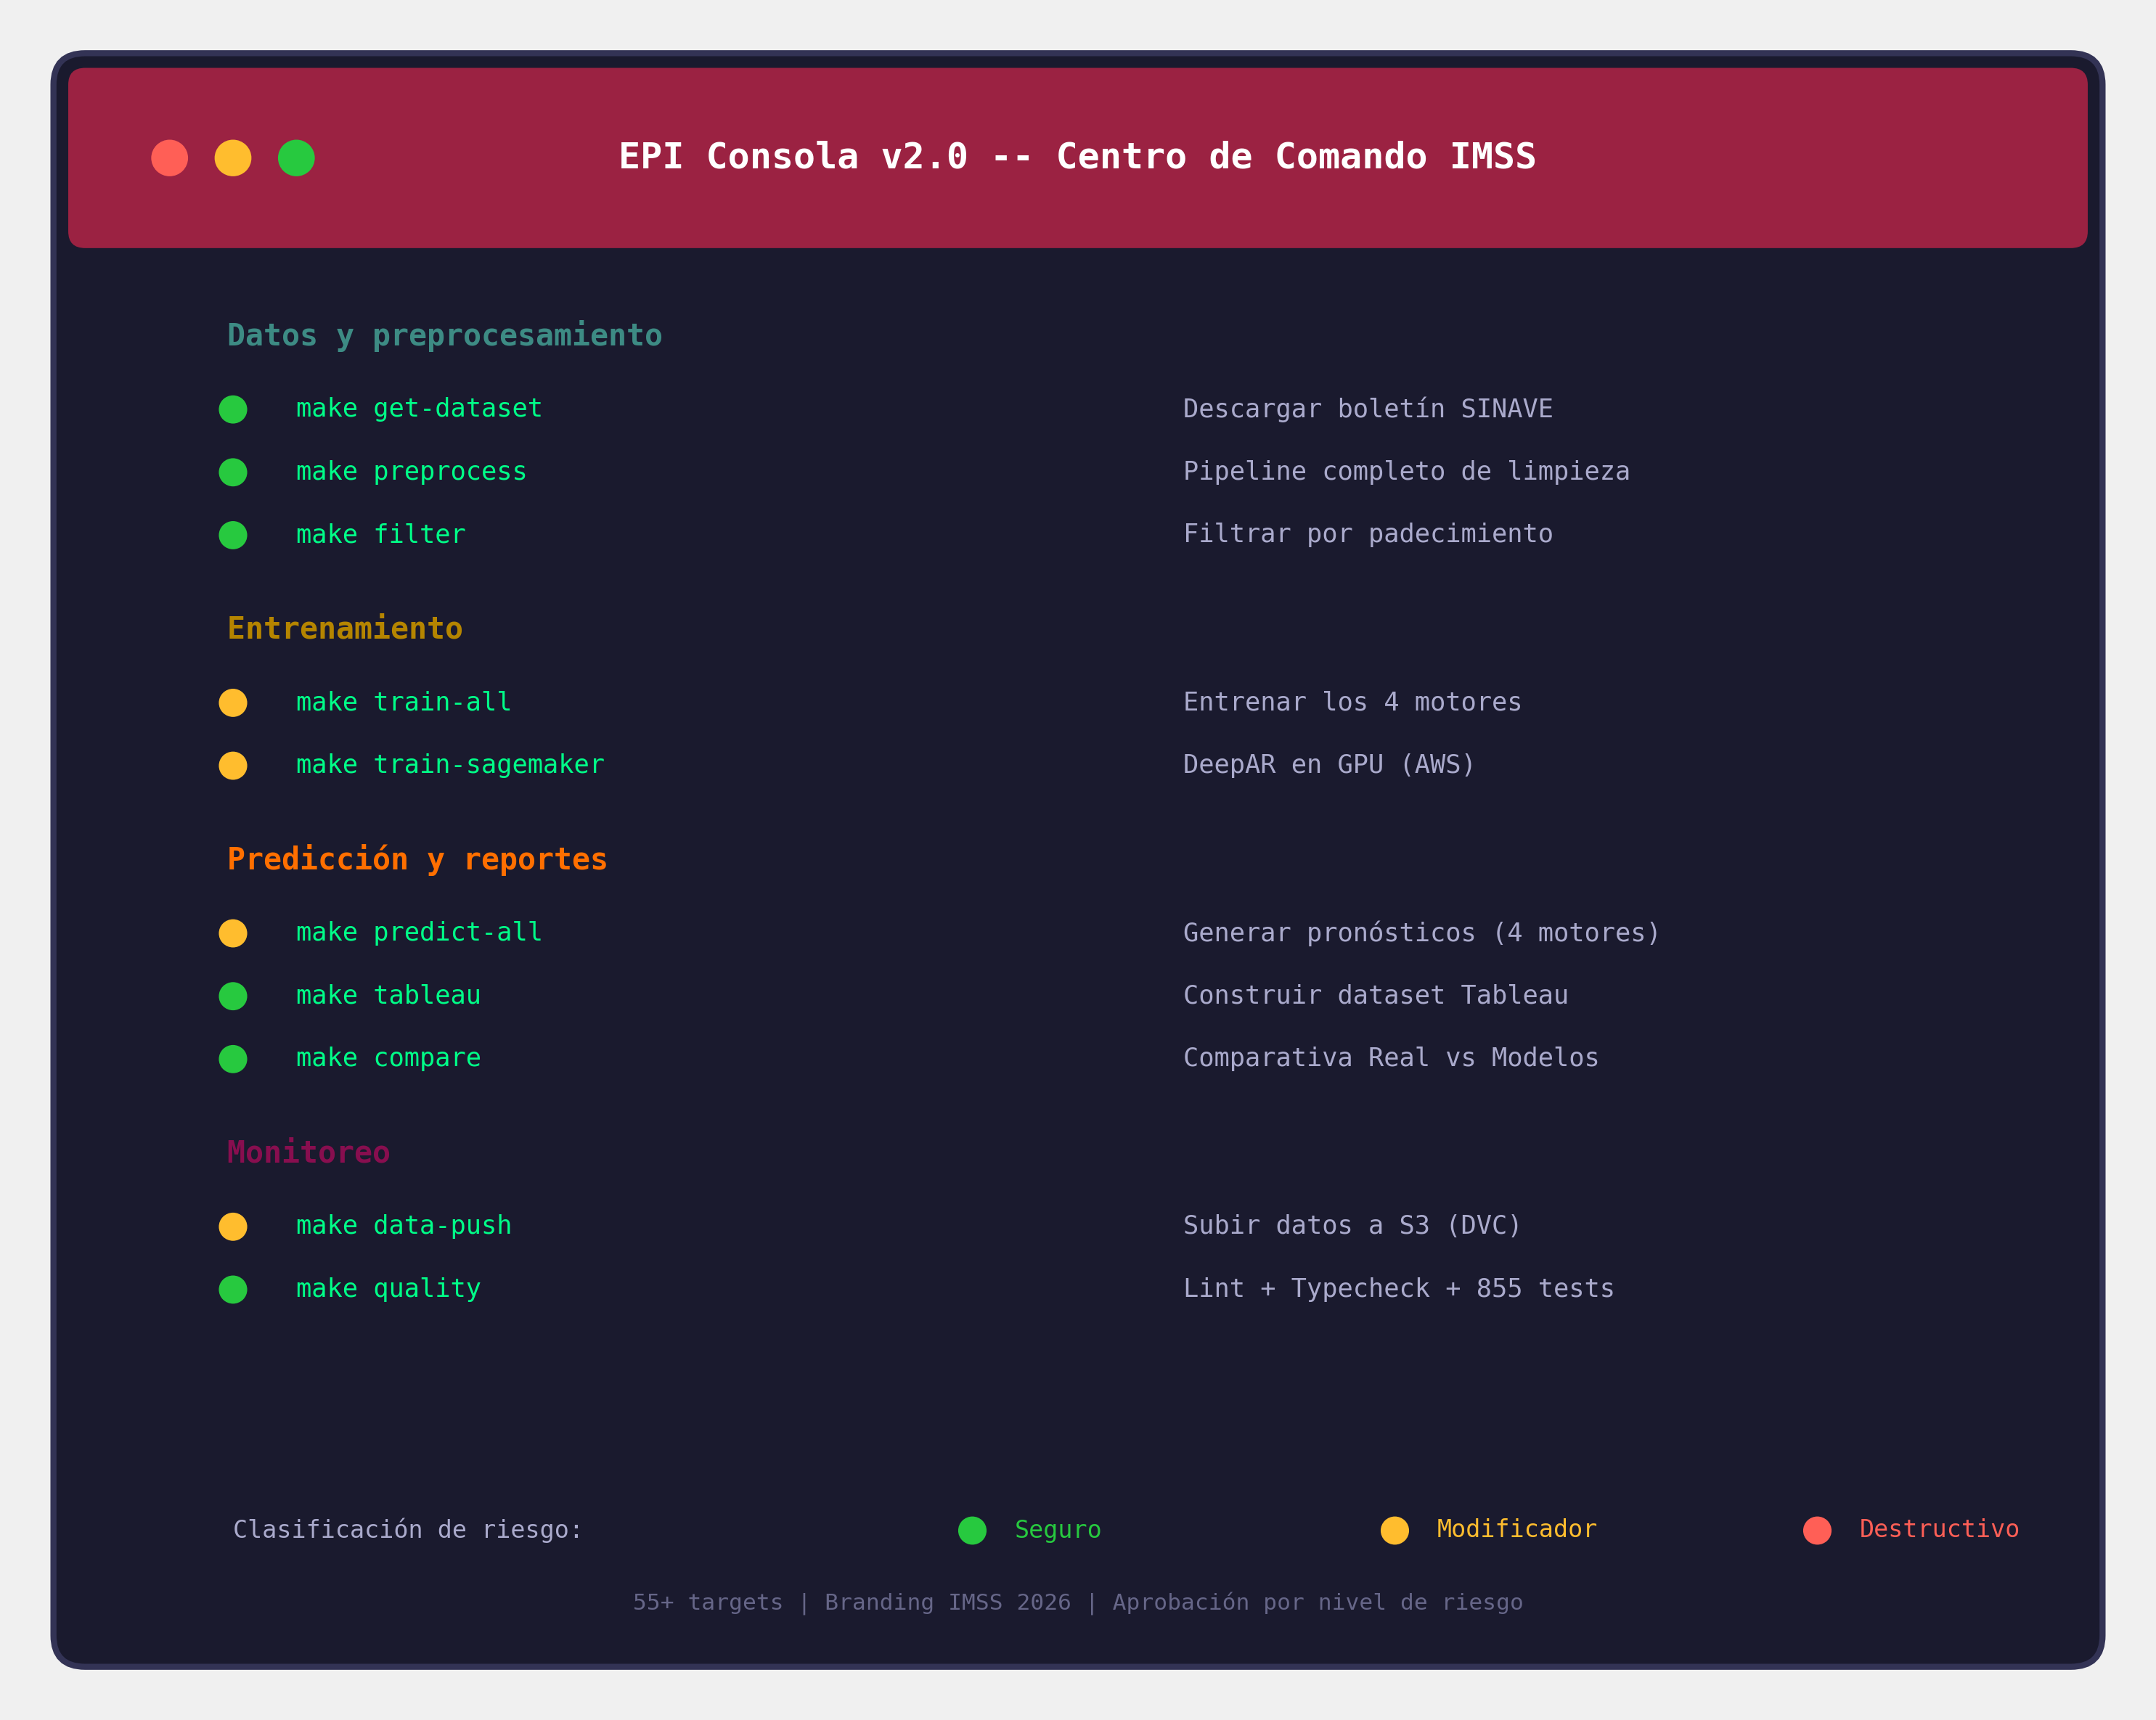
\includegraphics[width=1.15\textwidth]{consola_showcase.png}}
\caption[EPI Consola -- Menú de ayuda.]{EPI Consola con tema institucional \imss{}: menú de ayuda mostrando los 55+~targets organizados por categoría (Datos, Entrenamiento, SageMaker, Predicción, DVC) con clasificación de riesgo por colores.}
\label{fig:consola_showcase}
\end{figure}

\subsection{Público objetivo}

La EPI Consola está diseñada para \textbf{ingenieros MLOps, científicos de datos y personal técnico del \imss{}} que operan el ciclo de vida del sistema: desde la descarga de nuevos boletines SINAVE hasta el reentrenamiento trimestral de los 333~modelos. La interfaz reduce la curva de aprendizaje y minimiza errores operativos al centralizar todas las operaciones en un único punto de control.

% ============================================================
% 7. SHOWCASE: EPI WEB BOT
% ============================================================
\newpage
\section{EPI Web Bot: Inteligencia Epidemiológica al Alcance de Todos}\label{sec:epibot}

Si el EpiDashboard sirve a directivos y la EPI Consola al equipo técnico, el EPI Web Bot completa el ecosistema al llevar la inteligencia epidemiológica directamente a \textbf{médicos, personal de salud y público general}.

\subsection{Visión y propósito}

El EPI Web Bot es un asistente conversacional web que permite consultar pronósticos epidemiológicos en lenguaje natural, sin necesidad de conocimientos técnicos ni acceso a herramientas de análisis. Su diseño responde a una premisa: \textbf{los datos solo generan valor cuando llegan a quien los necesita para tomar decisiones}.

\begin{warningbox}
\textbf{Ejemplo de interacción:}\\[0.2cm]
\textbf{Médico:} ``?`Cuál es el pronóstico de depresión en Jalisco para los próximos 6 meses?''\\[0.2cm]
\textbf{EPI Web Bot:} ``Según nuestros modelos, Jalisco presenta un pronóstico de 38,500~casos de depresión (F32) para las próximas 26~semanas. El motor seleccionado es DeepAR, con un \smape{} de 4.2\%, lo que indica alta confiabilidad. Se observa un incremento estacional esperado entre marzo y mayo. Recomendación: considerar refuerzo en consultorios de psiquiatría para el periodo de mayor demanda.''
\end{warningbox}

\subsection{Capacidades principales}

\begin{itemize}
  \item \textbf{Consultas en lenguaje natural:} el médico no necesita conocer la estructura de datos ni las métricas; solo formula su pregunta como lo haría con un colega.
  \item \textbf{Respuestas contextualizadas:} cada respuesta incluye el dato solicitado, el nivel de confianza del modelo, y una recomendación práctica.
  \item \textbf{Base de conocimiento local:} 18+~handlers especializados que responden con datos reales del proyecto (métricas, boletín, modelos, semanas epidemiológicas) sin depender de servicios externos.
  \item \textbf{Explicaciones accesibles:} tendencias y alertas presentadas en lenguaje clínico, no estadístico.
  \item \textbf{Disponibilidad continua:} acceso vía web, complementando las consultas presenciales.
\end{itemize}

\begin{figure}[H]
\centering
\makebox[\textwidth][c]{%
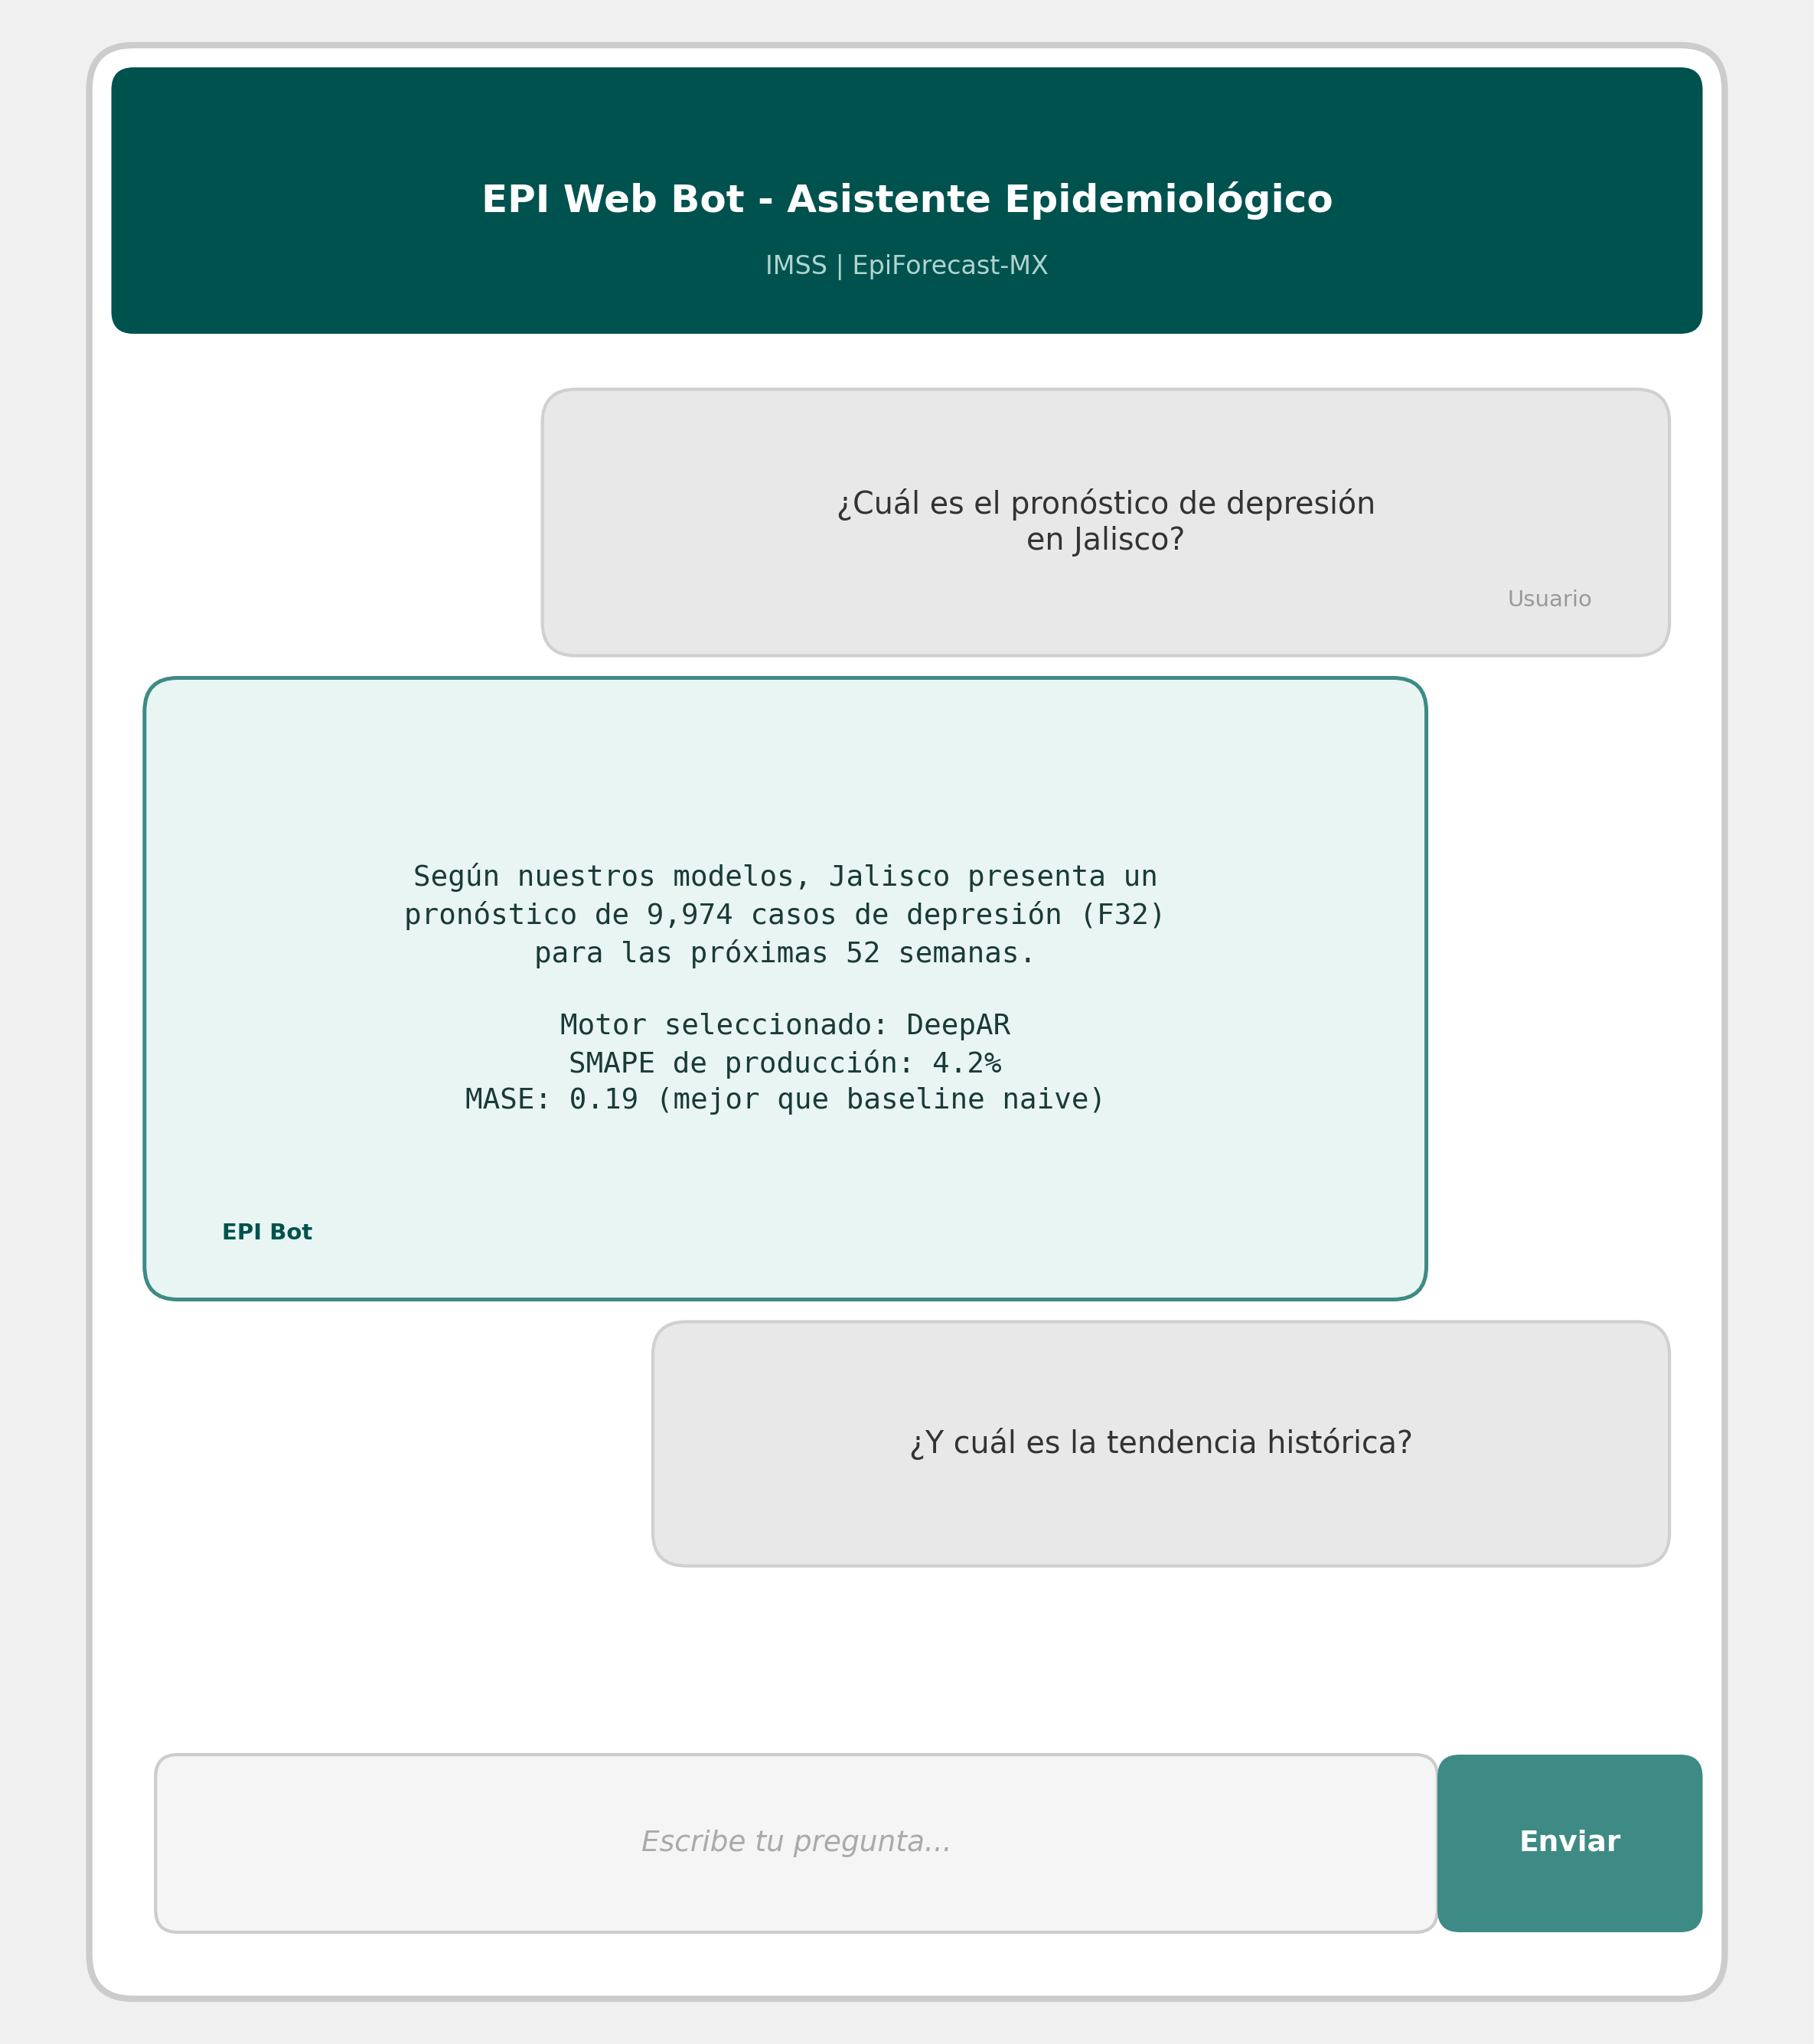
\includegraphics[width=1.0\textwidth]{epibot_showcase.png}}
\caption[EPI Web Bot -- Interfaz conversacional.]{Prototipo del EPI Web Bot: interfaz conversacional con branding \imss{} que permite a médicos y personal de salud consultar pronósticos epidemiológicos en lenguaje natural.}
\label{fig:epibot_showcase}
\end{figure}

\subsection{Públicos objetivo}

\begin{table}[H]
\centering
\caption{Públicos objetivo del EPI Web Bot}
\label{tab:publicos_epibot}
\small
\begin{tabularx}{\textwidth}{l X X}
\toprule
\textbf{Audiencia} & \textbf{Caso de uso} & \textbf{Beneficio} \\
\midrule
Médicos \imss{} & Consultar pronóstico por estado y padecimiento para planificación de consultas & Toma de decisiones informada en el punto de atención \\
\addlinespace
Personal de salud & Alertas tempranas de incremento estacional, orientación sobre tendencias & Preparación anticipada de recursos y turnos \\
\addlinespace
Público general & Información epidemiológica accesible, concientización & Democratización de datos de salud pública \\
\bottomrule
\end{tabularx}
\end{table}

\subsection{Arquitectura tecnológica}

El bot se sustenta en la base de conocimiento del proyecto (Knowledge Base), que contiene datos reales de las 333~series de producción, métricas de rendimiento y contexto epidemiológico. Para consultas que exceden el ámbito de la base local, utiliza un modelo de lenguaje (Gemini) como fallback, enriquecido con el contexto del proyecto para mantener la precisión y relevancia de las respuestas.

\begin{insightbox}
\textbf{Diferenciador clave:} EpiForecast-MX no solo construyó modelos de pronóstico, sino un \textbf{ecosistema completo de herramientas} para tres audiencias distintas: directivos (Dashboard), equipo técnico (Consola) y personal clínico (Web Bot). Este enfoque de ``último metro'' asegura que la inteligencia epidemiológica genere valor real en cada nivel de la organización.
\end{insightbox}

Presentado el ecosistema de herramientas que entrega los pronósticos a cada audiencia, las siguientes secciones abordan cómo operar, financiar y gobernar este sistema en un entorno institucional real.

% ============================================================
% 8. RECOMENDACIONES DE IMPLEMENTACION
% ============================================================
\newpage
\section{Recomendaciones de implementación}\label{sec:recomendaciones}

Basándose en los resultados del Avance~6 (Rebull et al., 2026c), esta sección sintetiza las recomendaciones clave para la operación productiva del sistema.

\subsection{Ciclo operativo propuesto}

\begin{figure}[H]
\centering
\makebox[\textwidth][c]{%
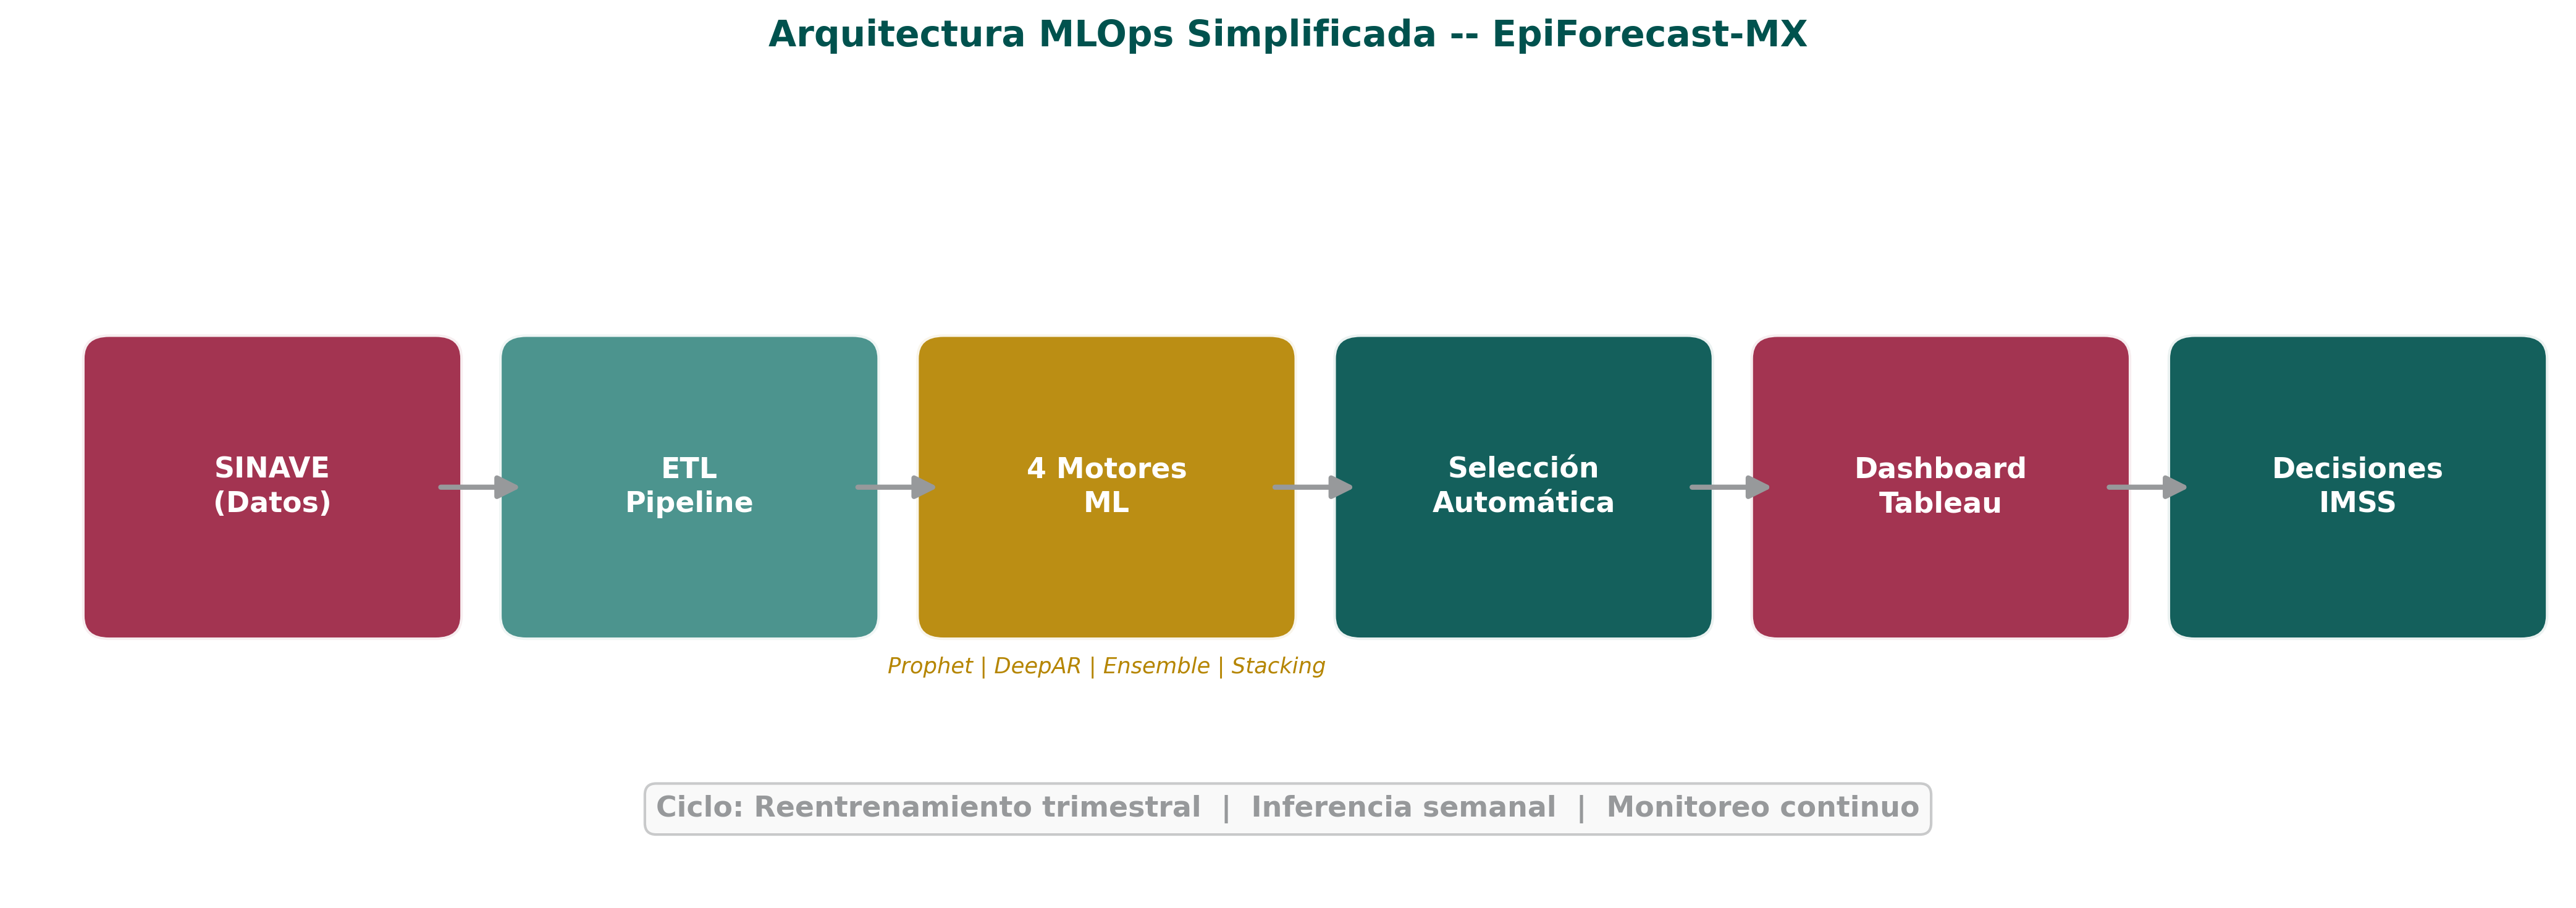
\includegraphics[width=1.15\textwidth]{arquitectura_simplificada.png}}
\caption[Arquitectura MLOps simplificada.]{Flujo operativo simplificado de EpiForecast-MX: desde la ingesta de datos SINAVE hasta la entrega de pronósticos a través del ecosistema de herramientas.}
\label{fig:arquitectura}
\end{figure}

Como ilustra la \figref{fig:arquitectura}, el sistema se diseñó para operar en dos ciclos complementarios:

\begin{table}[H]
\centering
\caption{Ciclos operativos del sistema}
\label{tab:ciclos_operativos}
\small
\begin{tabularx}{\textwidth}{l l X}
\toprule
\textbf{Ciclo} & \textbf{Frecuencia} & \textbf{Actividades} \\
\midrule
Inferencia & Semanal & Descarga de boletín SINAVE, ejecución de predicción batch, actualización del dashboard, validación contra datos reales \\
\addlinespace
Reentrenamiento & Trimestral & Reentrenamiento de los 333~modelos en GPU, validación cruzada completa, diagnóstico de overfitting y leakage, aprobación por epidemiólogo \\
\bottomrule
\end{tabularx}
\end{table}

\subsection{Estrategia de monitoreo}

El monitoreo continuo opera en tres dimensiones:

\begin{enumerate}
  \item \textbf{Data drift:} prueba de Kolmogorov-Smirnov sobre la distribución de los datos entrantes vs.~los datos de entrenamiento. Alerta si $p < 0.05$.
  \item \textbf{Degradación de métricas:} monitoreo de \smape{} y \mase{} en cada ciclo de validación semanal. Alerta si la métrica supera el percentil~95 histórico.
  \item \textbf{Anomalías operativas:} CloudWatch para monitoreo de infraestructura AWS (latencia, errores, consumo de recursos).
\end{enumerate}

\subsection{Expansión futura}

Con base en las reuniones con la Dra.~Ruth Perez-Hernandez, se identificaron cuatro ejes de expansión:

\begin{itemize}
  \item \textbf{Desagregación por rango de edad:} los datos SINAVE incluyen esta variable pero no fue explotada en la primera versión. Su incorporación permitiría pronósticos etarios críticos para planificación geriátrica.
  \item \textbf{Integración de datos de mortalidad:} correlacionar incidencia con mortalidad para identificar condiciones con mayor brecha entre diagnóstico y desenlace.
  \item \textbf{Análisis farmacológico:} cruzar pronósticos de incidencia con datos de consumo de medicamentos para anticipar demanda farmacéutica.
  \item \textbf{Escalabilidad a otras condiciones CIE-10:} la arquitectura multi-motor puede extenderse a cualquier condición reportada en SINAVE, multiplicando el impacto del sistema.
\end{itemize}

% ============================================================
% 9. ANALISIS COSTO--BENEFICIO
% ============================================================
\newpage
\section{Análisis costo--beneficio}\label{sec:costos}

Esta sección presenta un análisis de la inversión requerida y los beneficios generados por EpiForecast-MX, organizado por fases de la metodología CRISP-ML(Q) (Studer et al., 2021; Costa, 2022).

\subsection{Costos por fase CRISP-ML(Q)}

\begin{table}[H]
\centering
\caption{Inversión por fase CRISP-ML(Q)}
\label{tab:costos_crispml}
\small
\begin{tabularx}{\textwidth}{l r r X}
\toprule
\textbf{Fase CRISP-ML(Q)} & \textbf{USD} & \textbf{MXN\textsuperscript{*}} & \textbf{Componentes principales} \\
\midrule
1. Entendimiento del Negocio y Datos & 2,400 & 42,645 & Horas-persona (3~integrantes $\times$ 80~h), reuniones con IMSS, análisis de dominio \\
\addlinespace
2. Preparación de Datos & 1,800 & 31,984 & Pipeline ETL (scraping SINAVE, limpieza, feature engineering), almacenamiento S3 \\
\addlinespace
3. Modelado & 3,200 & 56,860 & Entrenamiento SageMaker (ml.g4dn.xlarge), experimentación con 4~motores, cross-validation \\
\addlinespace
4. Evaluación & 800 & 14,215 & CI/CD (GitHub Actions), testing automatizado (855~pruebas, 92\% cobertura), diagnósticos \\
\addlinespace
5. Despliegue & 600 & 10,661 & ECR (contenedores Docker), pipeline de inferencia, integración Tableau \\
\addlinespace
6. Monitoreo (anual) & 500 & 8,884 & CloudWatch, almacenamiento S3, reentrenamiento trimestral \\
\midrule
\textbf{Total (primer año)} & \textbf{9,300} & \textbf{165,249} & \\
\textbf{Operación anual recurrente} & \textbf{500} & \textbf{8,884} & Solo fases 5 y 6 \\
\bottomrule
\end{tabularx}
\begin{flushleft}
\scriptsize \textsuperscript{*} Tipo de cambio: 17.77~MXN/USD (Banxico FIX, marzo 2026).
\end{flushleft}
\end{table}

\begin{figure}[H]
\centering
\makebox[\textwidth][c]{%
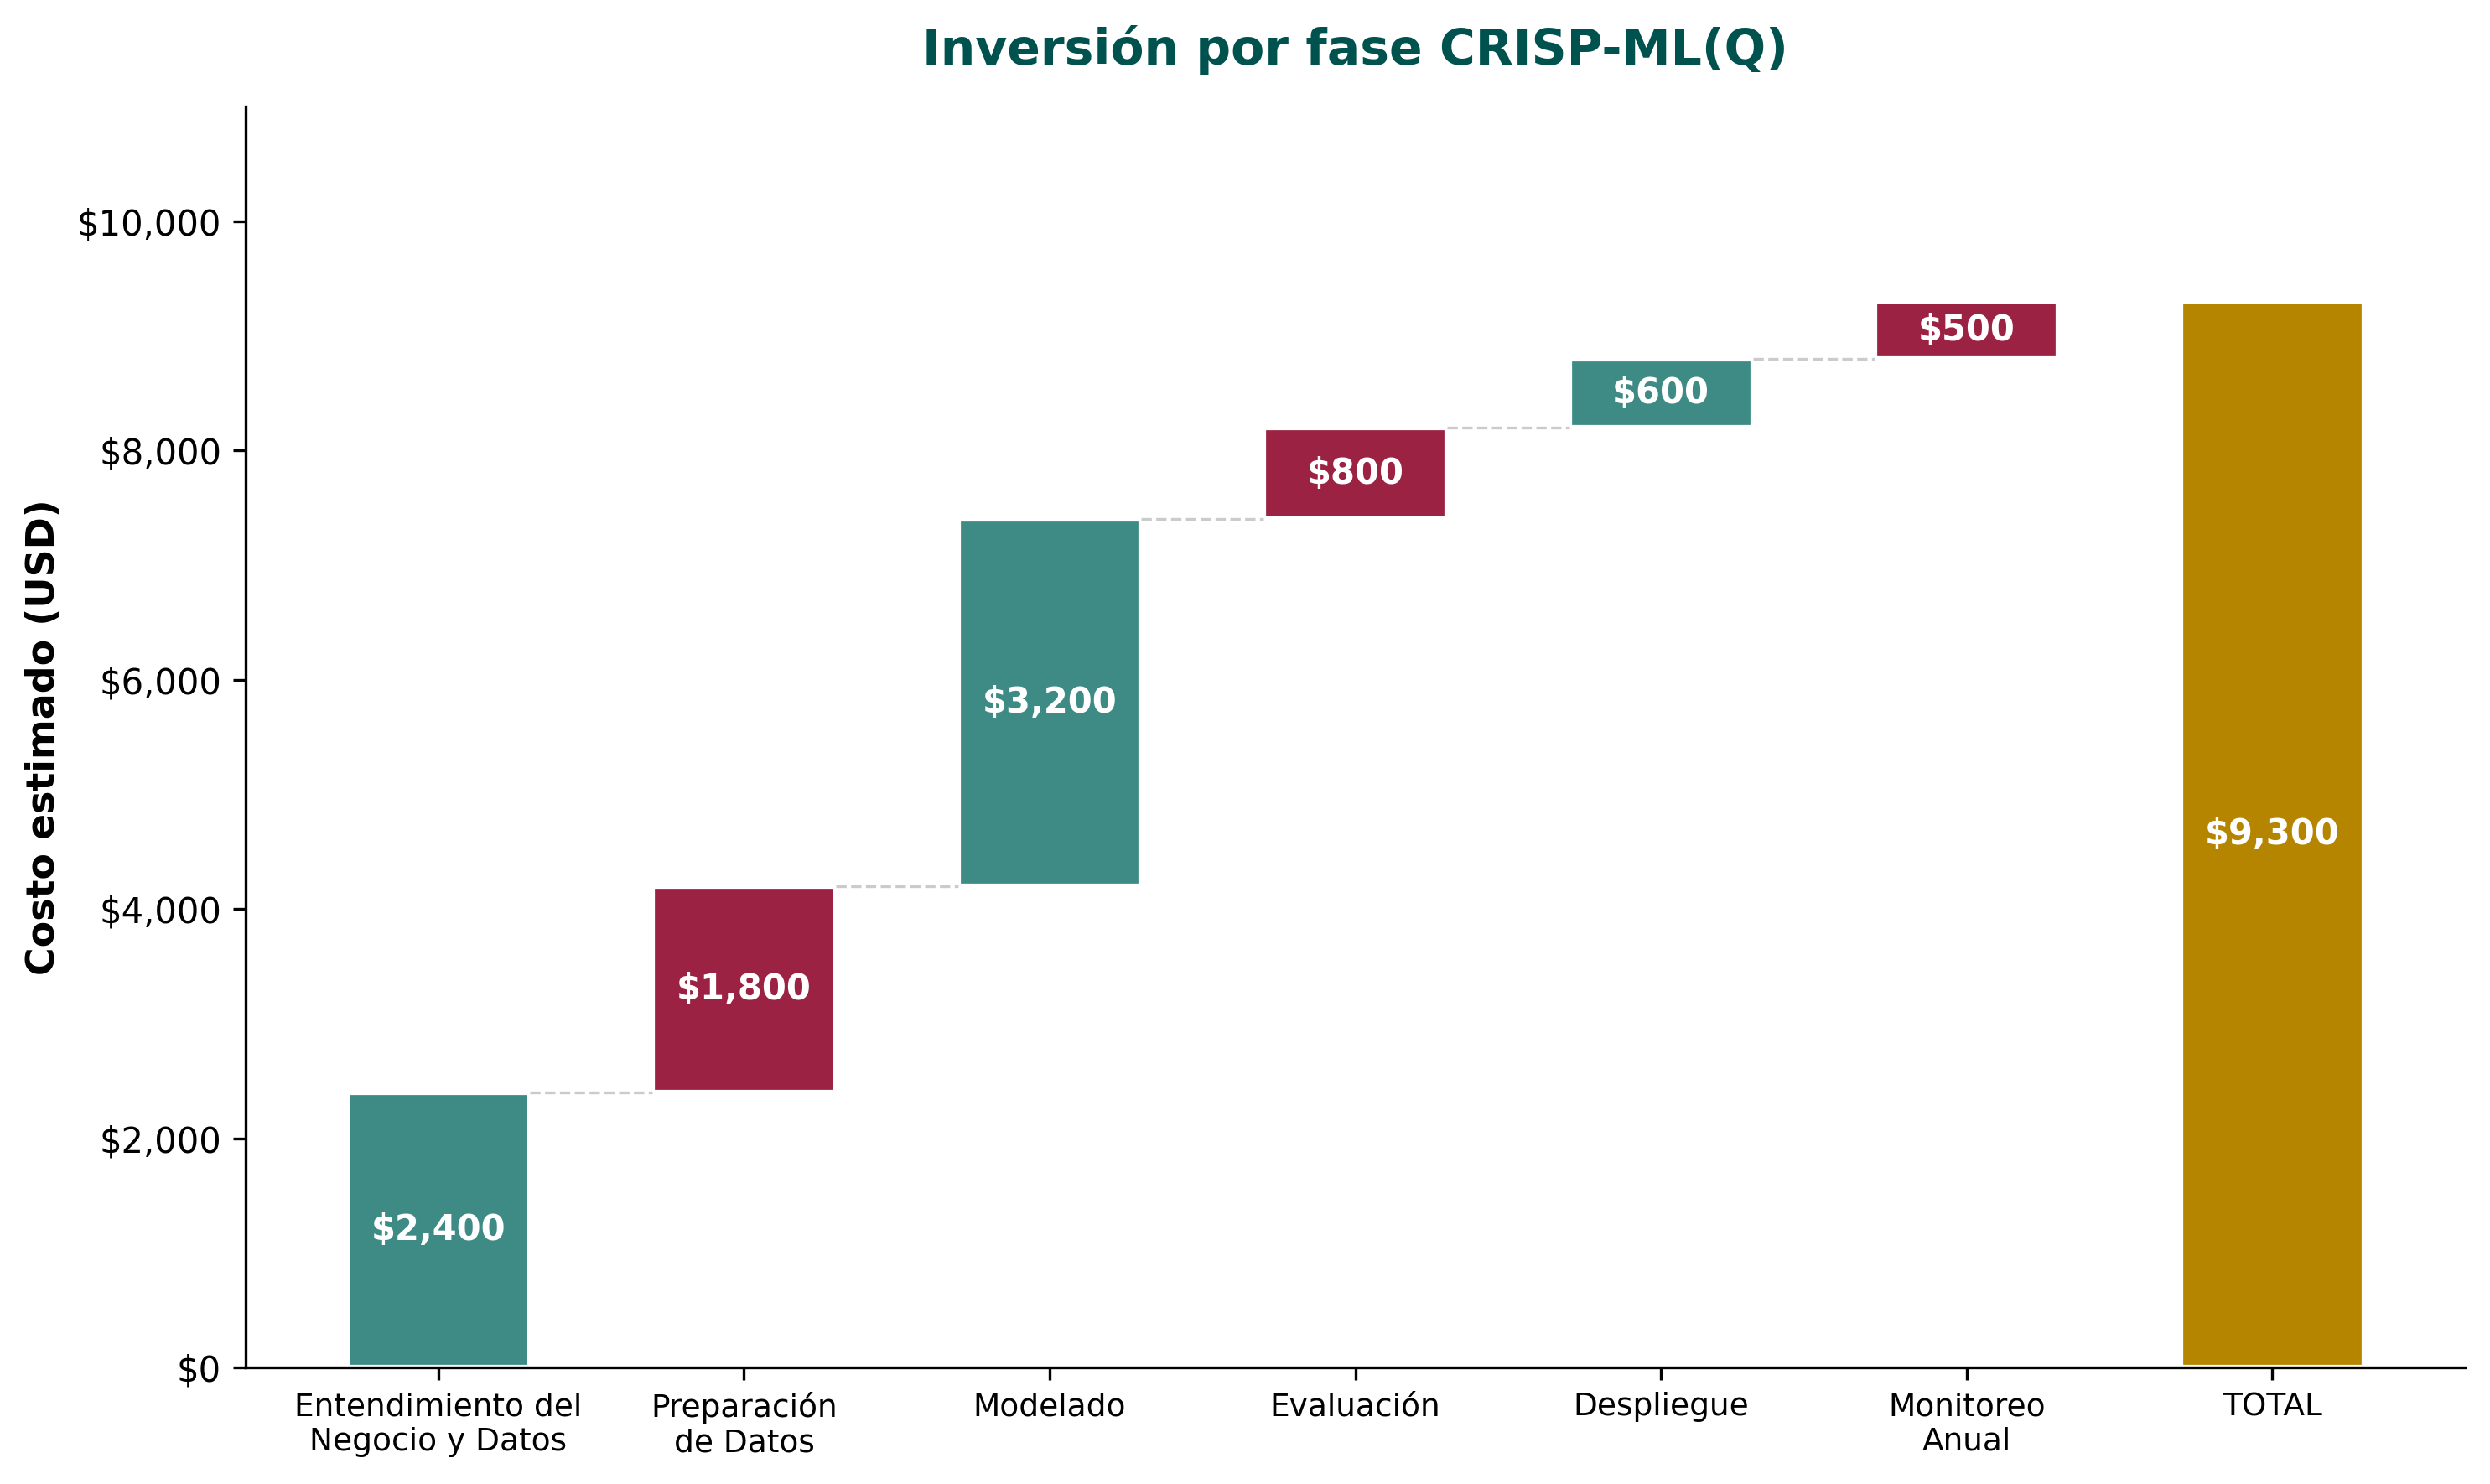
\includegraphics[width=1.15\textwidth]{costos_waterfall_crispml.png}}
\caption[Inversión por fase CRISP-ML(Q).]{Distribución de la inversión del proyecto por fase CRISP-ML(Q). La fase de Modelado concentra la mayor inversión (34\%), seguida por Entendimiento del Negocio (26\%).}
\label{fig:costos_waterfall}
\end{figure}

\subsection{Ahorro en infraestructura GPU}

La \figref{fig:costos_waterfall} desglosa la inversión por fase. La estrategia de reentrenamiento trimestral (en lugar de semanal) genera ahorros significativos en el componente más costoso del sistema: el entrenamiento en GPU.

\begin{kpibox}
\begin{center}
{\Large\bfseries\color{teal} 92\% de ahorro en costos GPU de entrenamiento}\\[0.3cm]
\normalsize De 52 a 4~ciclos anuales de entrenamiento en ml.g4dn.xlarge\\[0.3cm]
{\large\color{burgundy} Costo por ciclo: \$3.50 -- \$8.50 USD \quad|\quad Anual: \$14 -- \$34 USD (vs.~\$182 -- \$442)}
\end{center}
\end{kpibox}

\vspace{0.3cm}

El ahorro operativo total (considerando S3, ECR, CloudWatch y transferencia de datos) supera el 40\% respecto a un esquema de reentrenamiento semanal, resultando en un costo operativo anual proyectado de \textbf{240 -- 506~USD} (4,265 -- 8,990~MXN) (AWS, 2025). La \figref{fig:costos_vs_beneficios} muestra la asimetría entre costos e impacto.

\subsection{Beneficios cuantificables}

\begin{table}[H]
\centering
\caption{Análisis de beneficios del sistema}
\label{tab:beneficios}
\small
\begin{tabularx}{\textwidth}{l X r}
\toprule
\textbf{Beneficio} & \textbf{Descripción} & \textbf{Estimación} \\
\midrule
Reducción de desperdicio farmacológico & Anticipar demanda de medicamentos reduce sobre-aprovisionamiento en 5--15\% (McKinsey, 2024; Deloitte, 2024) & 200--600~M~MXN/año \\
\addlinespace
Optimización de recursos humanos & Distribución de especialistas basada en demanda proyectada, no histórica & Mejor cobertura \\
\addlinespace
Ahorro GPU (92\%) & Reentrenamiento trimestral vs.~semanal & \$168 -- \$408 USD/año \\
\addlinespace
Ahorro operativo total (>40\%) & Infraestructura completa optimizada & \$200+~USD/año \\
\bottomrule
\end{tabularx}
\end{table}

\begin{kpibox}
\begin{center}
{\Large\bfseries\color{burgundy} Retorno de inversión: por cada peso invertido,}\\[0.2cm]
{\fontsize{28}{34}\selectfont\bfseries\color{teal} \$22,000+ pesos}\\[0.2cm]
{\large en ahorro potencial de gestión farmacéutica}
\end{center}
\end{kpibox}

\begin{figure}[H]
\centering
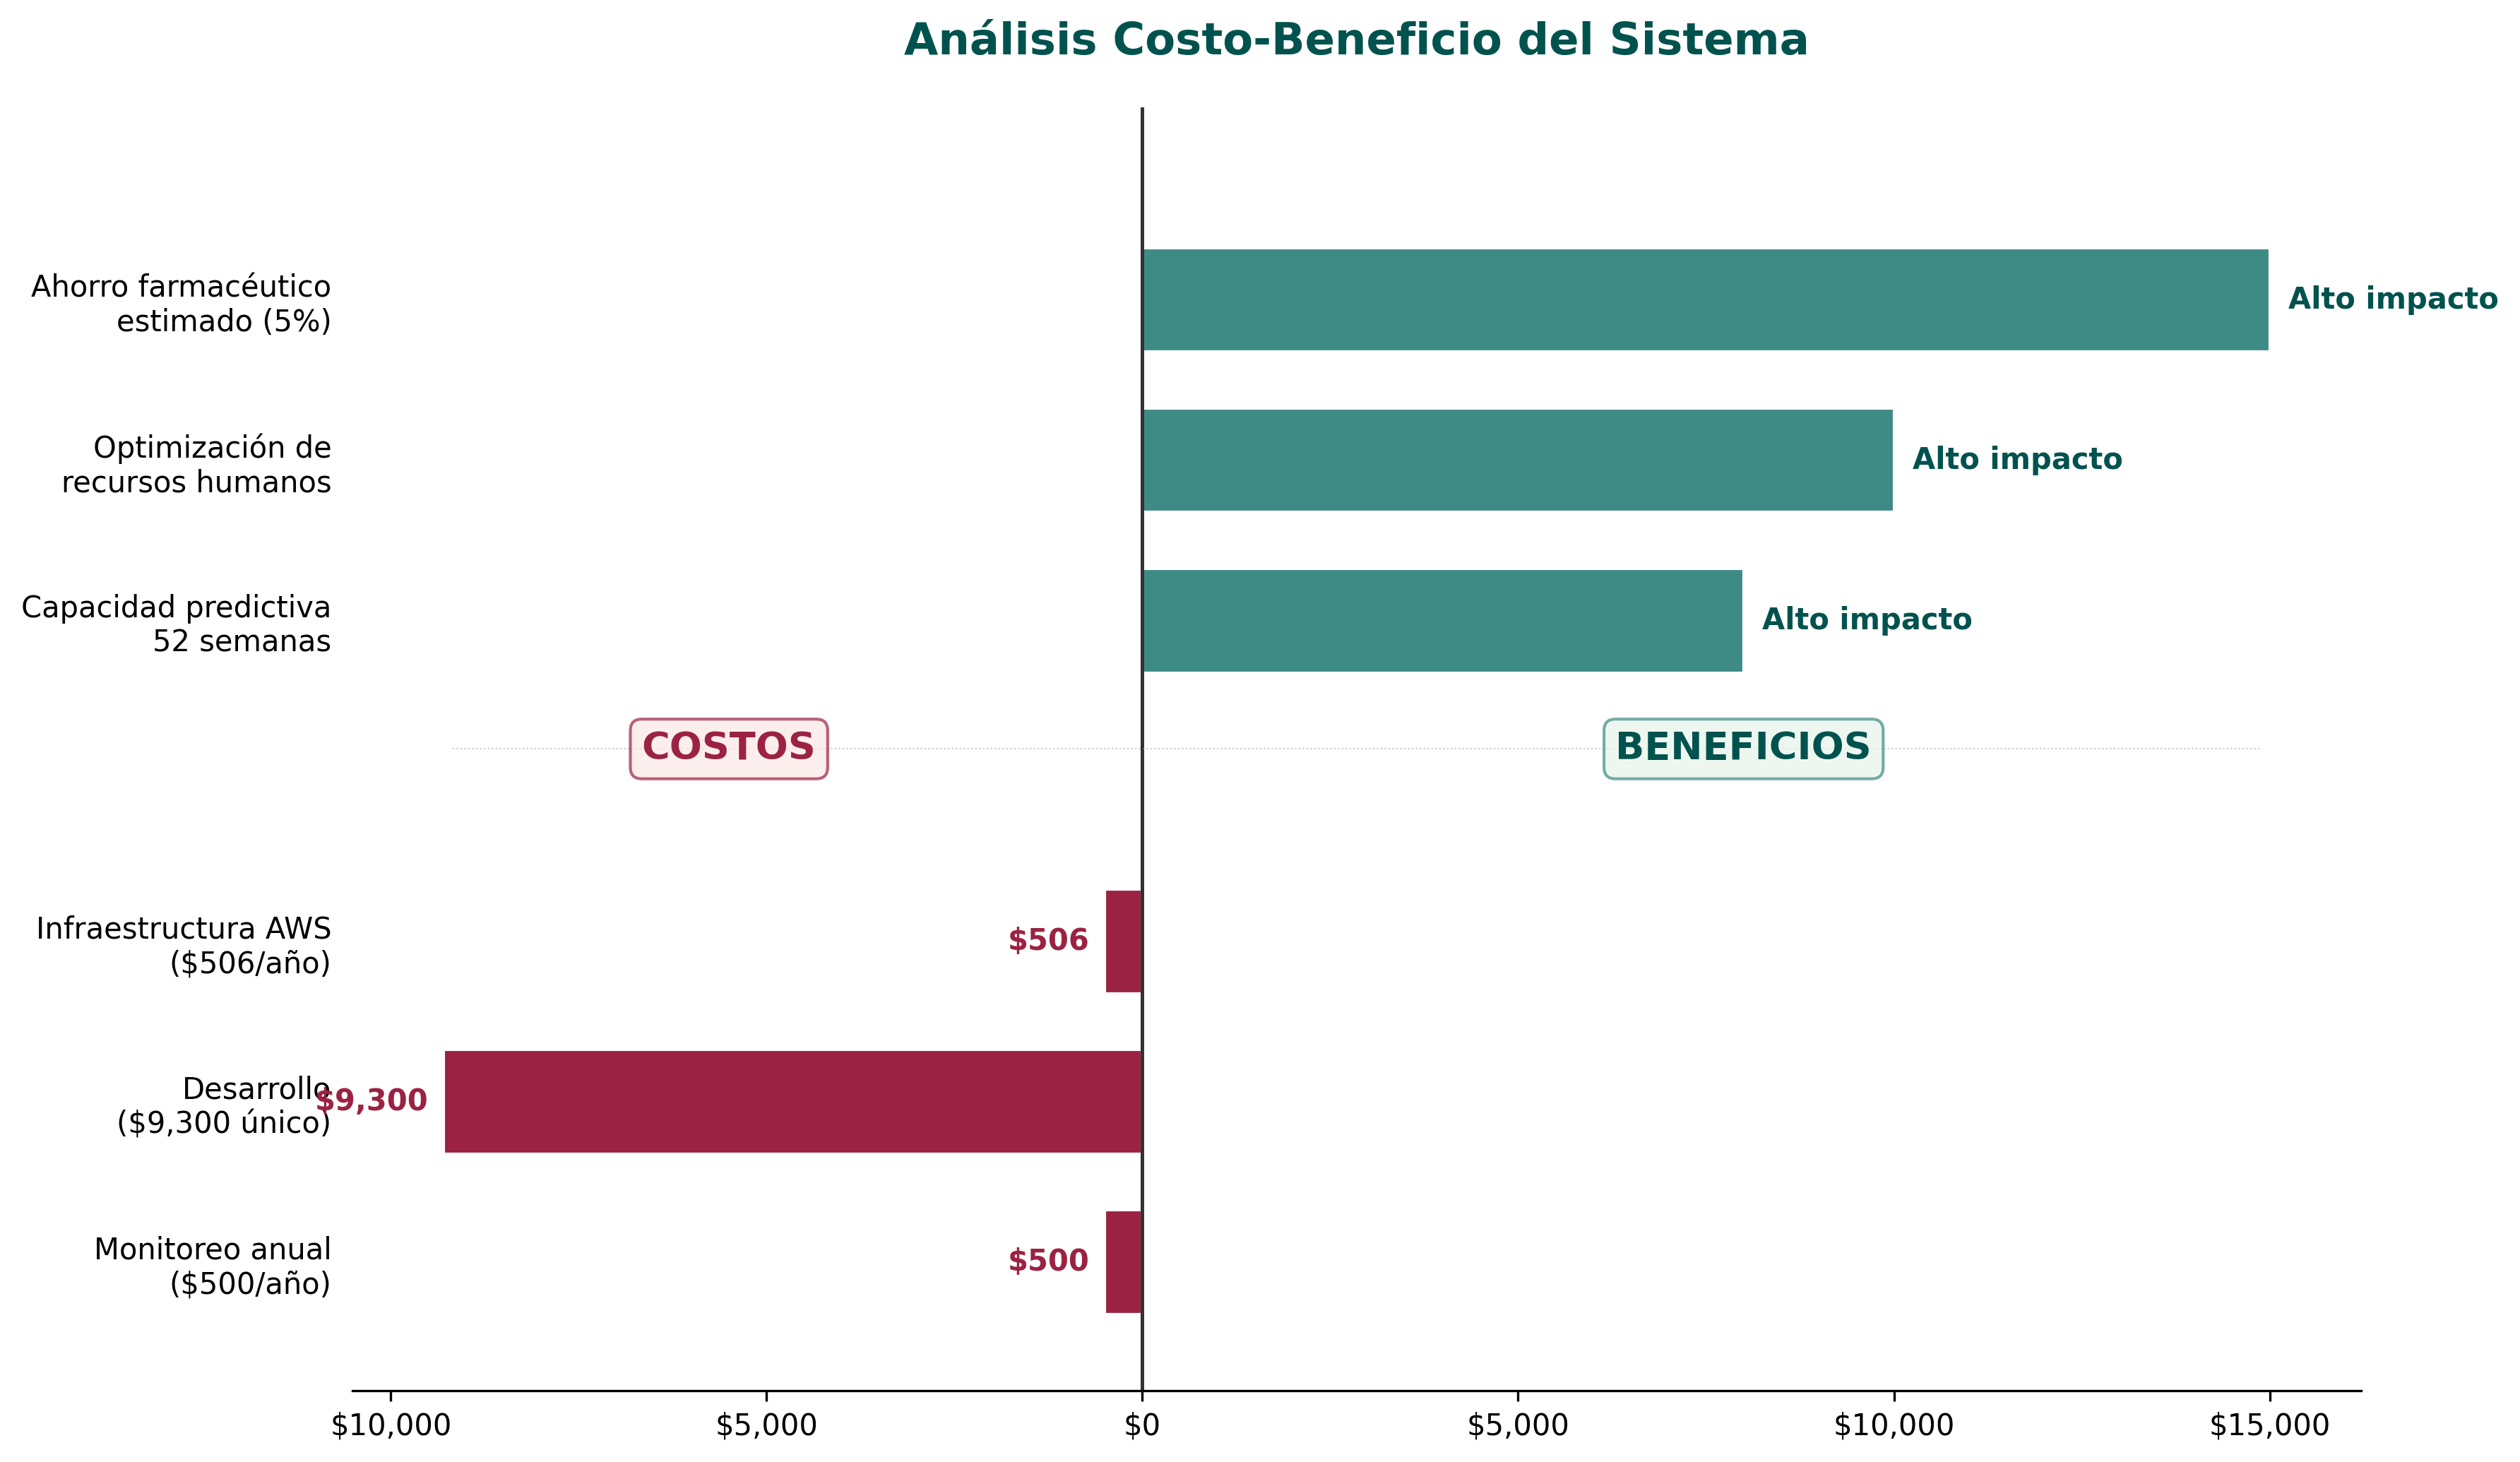
\includegraphics[width=0.95\textwidth]{costos_vs_beneficios.png}
\caption[Costos vs.\ beneficios estimados.]{Costos del sistema vs.\ beneficios estimados. La asimetría entre la inversión requerida (izquierda) y el ahorro farmacéutico conservador (derecha) evidencia un ROI de 22,000:1.}
\label{fig:costos_vs_beneficios}
\end{figure}

\begin{insightbox}
\textbf{Supuestos del cálculo de ROI:}
\begin{itemize}
  \item Gasto del \imss{} en medicamentos neurológicos y psiquiátricos (F32, G20, G30): \textbf{\$4,000~millones MXN/año} estimados. El gasto total del \imss{} en medicamentos fue de \$81,891~millones en 2024 (Cuenta Pública, ASF). La proporción para los tres padecimientos se estimó a partir del mercado mexicano de fármacos para trastornos depresivos (\$337.6~M~USD, Statista 2024) y la cobertura del \imss{} ($\approx$50\% de la población asegurada).
  \item Reducción de desperdicio farmacéutico: \textbf{5\%} (estimación conservadora; la literatura reporta 10--30\% con sistemas de pronóstico de demanda).
  \item Ahorro conservador: 4,000~M $\times$ 5\% = \textbf{200~millones MXN/año}.
  \item Costo del sistema: \textbf{8,992~MXN/año} (límite superior).
  \item Ratio: 200,000,000 / 8,992 $\approx$ \textbf{22,000:1}.
\end{itemize}
\scriptsize Fuentes: Cuenta Pública IMSS 2024 (ASF), CIEP 2024, Statista 2024, McKinsey 2024, Deloitte 2024. Tipo de cambio: 17.77~MXN/USD (Banxico FIX, marzo 2026). Costo por consulta de especialidad IMSS 2026: \$2,082~MXN (DOF, 10/12/2025).
\end{insightbox}

\subsection{Beneficios intangibles}

Más allá de los ahorros cuantificables, EpiForecast-MX genera beneficios de \textbf{alto valor estratégico}:

\begin{enumerate}
  \item \textbf{Capacidad predictiva antes inexistente:} el \imss{} pasa de operar reactivamente a tener visión anticipada de 52~semanas para tres condiciones críticas.
  \item \textbf{Equidad en atención:} la desagregación por género y región visibiliza disparidades que antes permanecían ocultas en los agregados nacionales.
  \item \textbf{Base para toma de decisiones basada en evidencia:} los pronósticos proveen un sustento cuantitativo para decisiones presupuestales y de política pública.
  \item \textbf{Escalabilidad demostrada:} la arquitectura multi-motor puede extenderse a las miles de condiciones CIE-10 reportadas en SINAVE, multiplicando el retorno de la inversión.
  \item \textbf{Precedente institucional:} EpiForecast-MX puede ser el piloto que demuestre al \imss{} el valor de la inteligencia artificial aplicada a la epidemiología, abriendo la puerta a inversiones mayores.
\end{enumerate}

\begin{insightbox}
\textbf{Relación costo--impacto:} El costo operativo anual del sistema (240--506~USD) equivale a 4~consultas de especialidad al costo unitario \imss{} 2026. A cambio, el \imss{} obtiene pronósticos para 333~series, cubriendo 3~padecimientos en 32~estados con desagregación por género: un sistema que monitorea más de 165,000~casos pronosticados al año a nivel nacional.
\end{insightbox}

Si bien el análisis de costos confirma la viabilidad económica del sistema, toda implementación en el sector salud conlleva riesgos que deben identificarse y mitigarse de forma proactiva.

% ============================================================
% 10. RIESGOS Y DESAFIOS
% ============================================================
\newpage
\section{Riesgos y desafíos}\label{sec:riesgos}

Siguiendo el marco de referencia del NIST AI Risk Management Framework (NIST, 2023) y la clasificación del Wharton AIRS (Wharton AIRS, 2023), se identifican los principales riesgos del sistema organizados en cuatro categorías.

\subsection{Riesgos relacionados con los datos}

\begin{table}[H]
\centering
\caption{Riesgos relacionados con los datos}
\label{tab:riesgos_datos}
\scriptsize
\setlength{\tabcolsep}{3pt}
\begin{tabularx}{\textwidth}{X c c X}
\toprule
\textbf{Riesgo} & \textbf{Prob.} & \textbf{Impacto} & \textbf{Estrategia de mitigación} \\
\midrule
Subregistro epidemiológico: los datos SINAVE reflejan casos \emph{reportados}, no incidencia real & \riskHigh & \riskMed & Interpretar pronósticos como tendencias relativas, no cifras absolutas; complementar con encuestas poblacionales \\
\addlinespace
Discontinuidad de boletines o cambios de formato en SINAVE & \riskMed & \riskHigh & Pipeline de scraping con validaciones automáticas; alertas ante cambios estructurales; pruebas de regresión \\
\addlinespace
Calidad variable entre estados: algunos estados reportan con menor rigurosidad & \riskHigh & \riskMed & Fallback regional para series con menos de 5~casos/52~semanas; monitoreo de completitud \\
\addlinespace
Sesgo temporal por COVID-19: patrones 2020--2022 no representativos & \riskLow & \riskMed & Marcadores de régimen en Prophet; ventana de entrenamiento post-pandemia ponderada \\
\bottomrule
\end{tabularx}
\end{table}

\subsection{Riesgos de ataques}

\begin{table}[H]
\centering
\caption{Riesgos de ataques al sistema}
\label{tab:riesgos_ataques}
\scriptsize
\setlength{\tabcolsep}{3pt}
\begin{tabularx}{\textwidth}{X c c X}
\toprule
\textbf{Riesgo} & \textbf{Prob.} & \textbf{Impacto} & \textbf{Estrategia de mitigación} \\
\midrule
Data poisoning: manipulación de reportes SINAVE upstream & \riskLow & \riskHigh & Validaciones estadísticas en el pipeline de ingesta; alertas ante anomalías de magnitud; auditoría de fuentes \\
\addlinespace
Adversarial inputs en el pipeline de inferencia & \riskLow & \riskMed & Rangos de sanidad en inputs; tests automatizados; validación humana semanal \\
\addlinespace
Acceso no autorizado a endpoints SageMaker & \riskLow & \riskHigh & IAM policies restrictivas; VPC privada; rotación de credenciales; CloudTrail para auditoría \\
\bottomrule
\end{tabularx}
\end{table}

\subsection{Riesgos de prueba y confianza}

\begin{table}[H]
\centering
\caption{Riesgos de prueba y confianza}
\label{tab:riesgos_confianza}
\scriptsize
\setlength{\tabcolsep}{3pt}
\begin{tabularx}{\textwidth}{X c c X}
\toprule
\textbf{Riesgo} & \textbf{Prob.} & \textbf{Impacto} & \textbf{Estrategia de mitigación} \\
\midrule
Concept drift: cambio en patrones epidemiológicos post-pandemia & \riskHigh & \riskHigh & Monitoreo de drift (Kolmogorov-Smirnov); reentrenamiento trimestral; alertas automáticas \\
\addlinespace
Explicabilidad limitada de DeepAR (modelo de caja negra) & \riskMed & \riskMed & Complementar con Prophet (interpretable) en series críticas; documentar intervalos de confianza; reportar métricas de incertidumbre \\
\addlinespace
Sobreajuste en series de baja incidencia & \riskMed & \riskMed & Diagnóstico automatizado de overfitting (ratio test/train); fallback regional; umbral de 5~casos mínimos \\
\addlinespace
Validación clínica pendiente: los modelos no han sido validados formalmente por epidemiólogos & \riskMed & \riskHigh & Protocolo de validación semanal con datos reales del boletín; reuniones con Dra.~Ruth y Dra.~Lina; publicación científica en proceso \\
\bottomrule
\end{tabularx}
\end{table}

\subsection{Riesgos de cumplimiento}

\begin{table}[H]
\centering
\caption{Riesgos de cumplimiento normativo}
\label{tab:riesgos_cumplimiento}
\scriptsize
\setlength{\tabcolsep}{3pt}
\begin{tabularx}{\textwidth}{X c c X}
\toprule
\textbf{Riesgo} & \textbf{Prob.} & \textbf{Impacto} & \textbf{Estrategia de mitigación} \\
\midrule
Normativa de datos de salud: NOM-024-SSA3 y Ley de Protección de Datos Personales & \riskLow & \riskHigh & Los datos SINAVE son agregados y anónimos (no contienen datos personales); documentar cumplimiento \\
\addlinespace
Uso ético de predicciones epidemiológicas: riesgo de estigmatización o discriminación regional & \riskLow & \riskMed & Presentar pronósticos como herramienta de planificación, no de evaluación de desempeño estatal; guía de uso ético \\
\addlinespace
Gobernanza del modelo: ausencia de framework formal de aprobación de cambios & \riskMed & \riskMed & Propuesta de comité de gobernanza (epidemiólogo + ingeniero + directivo); bitácora de versiones; auditoría trimestral \\
\bottomrule
\end{tabularx}
\end{table}

\begin{figure}[H]
\centering
\makebox[\textwidth][c]{%
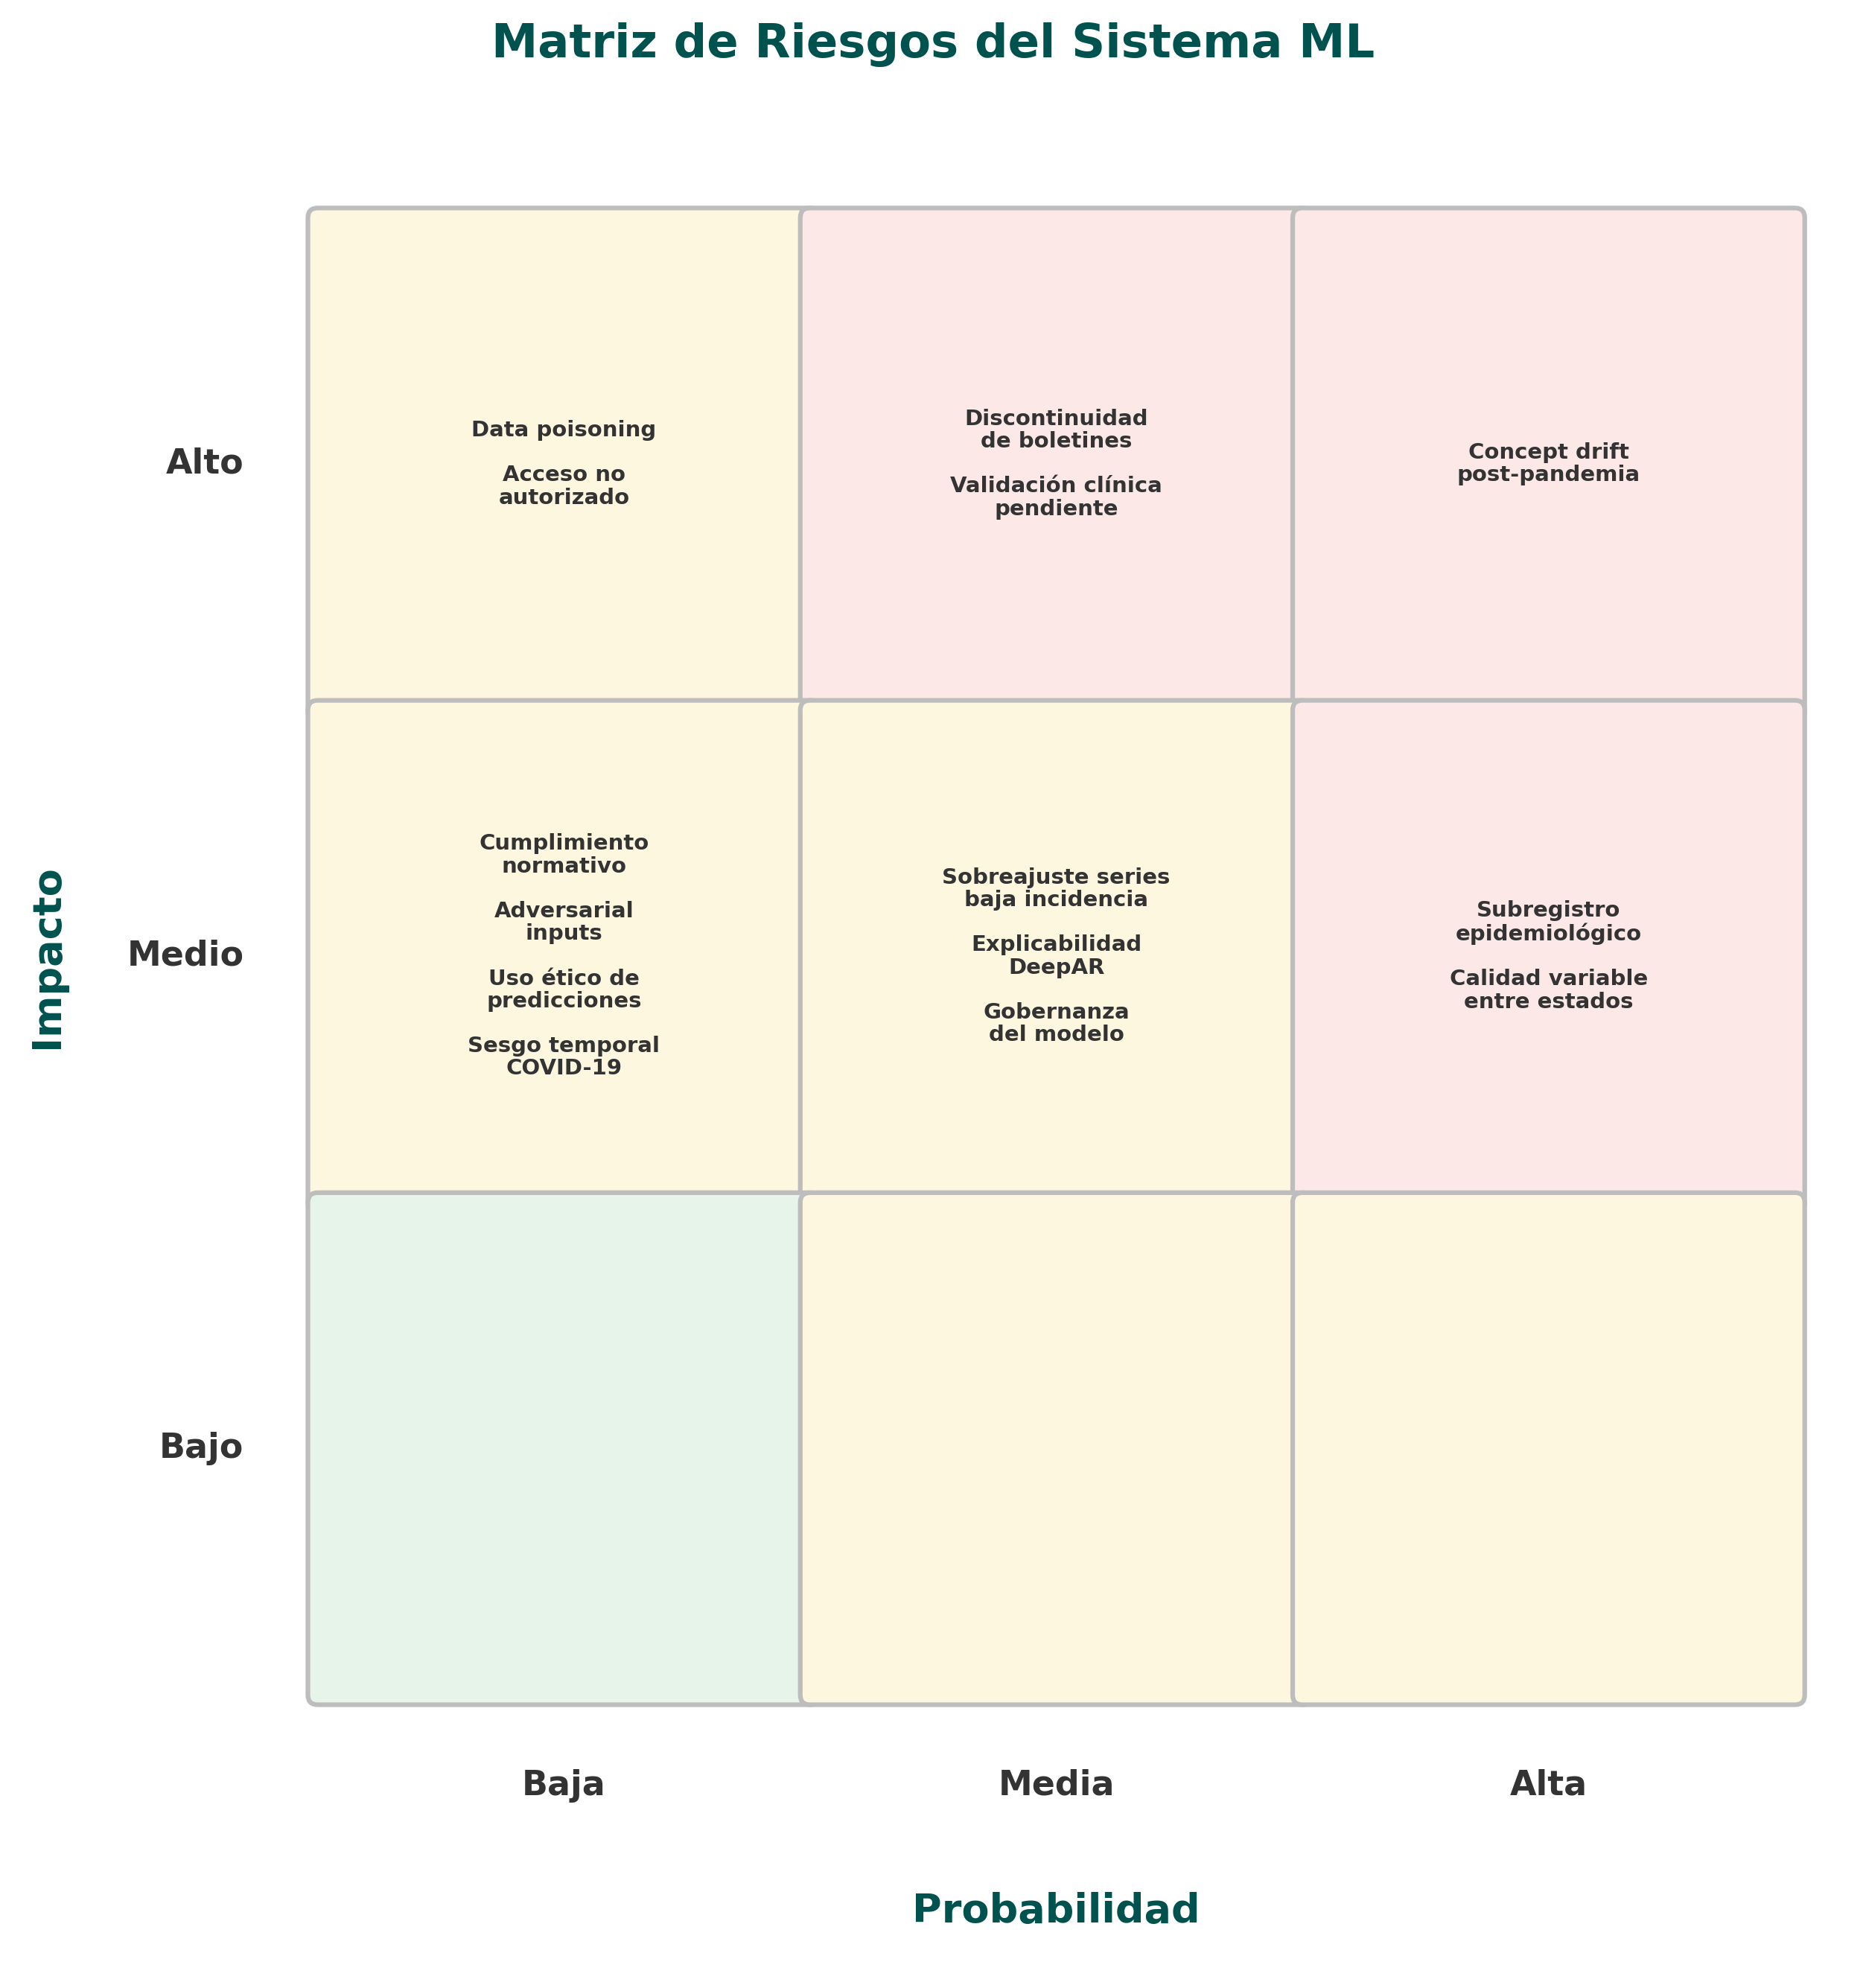
\includegraphics[width=1.0\textwidth]{riesgos_heatmap.png}}
\caption[Matriz de riesgos del sistema ML.]{Matriz de riesgos de probabilidad $\times$ impacto. Los riesgos de concept drift y validación clínica pendiente se ubican en la zona de mayor atención (alta probabilidad, alto impacto).}
\label{fig:riesgos_heatmap}
\end{figure}

\begin{criticalbox}
\textbf{Riesgo crítico identificado} (ver \figref{fig:riesgos_heatmap})\textbf{:} El concept drift post-pandemia es el riesgo de mayor prioridad. La estrategia de reentrenamiento trimestral con monitoreo continuo de drift está diseñada específicamente para mitigarlo. La validación semanal contra datos reales del boletín SINAVE proporciona una señal temprana de degradación del modelo (Babic et al., 2021).
\end{criticalbox}

% ============================================================
% 11. CONCLUSIONES GENERALES
% ============================================================
\newpage
\section{Conclusiones generales}\label{sec:conclusiones}

EpiForecast-MX demuestra que es posible construir un sistema de pronóstico epidemiológico de alta precisión para el \imss{} con una inversión modesta y tecnología accesible. Los principales logros del proyecto son:

\begin{enumerate}
  \item \textbf{333~modelos de producción} que cubren tres padecimientos neurológicos en las 32~entidades federativas de México, desagregados por sexo, con un horizonte de 52~semanas.

  \item \textbf{Precisión superior a la línea base} en el 94.9\% de las series (\mase{} < 1), con una mediana global de \mase{} de 0.30, un 70\% mejor que el pronóstico naive estacional.

  \item \textbf{Arquitectura multi-motor} que selecciona automáticamente el mejor algoritmo para cada serie, eliminando el sesgo de un enfoque único y maximizando la precisión agregada.

  \item \textbf{Ecosistema completo de herramientas} (Dashboard, Consola y Web Bot) que lleva la inteligencia epidemiológica desde el modelo hasta el punto de decisión, cubriendo tres audiencias distintas.

  \item \textbf{Infraestructura MLOps productiva} con reentrenamiento trimestral automatizado, inferencia semanal, monitoreo de drift y un costo operativo anual de 240--506~USD.

  \item \textbf{Validación con datos reales:} el sistema fue validado contra boletines SINAVE no vistos durante el entrenamiento, confirmando que los pronósticos son confiables fuera de muestra.
\end{enumerate}

\subsection{Comparativa con proyectos anteriores}

EpiForecast-MX se construyó sobre el trabajo pionero de tres equipos que abordaron cada padecimiento de manera individual (Equipo~16: Depresión, Equipo~20: Parkinson, Equipo~22: Alzheimer). La \tabref{tab:comparativa} resume la evolución:

\begin{table}[H]
\centering
\caption{Comparativa entre proyectos anteriores y EpiForecast-MX}
\label{tab:comparativa}
\scriptsize
\setlength{\tabcolsep}{4pt}
\begin{tabularx}{\textwidth}{l X X}
\toprule
\textbf{Aspecto} & \textbf{Equipos Anteriores (16, 20, 22)} & \textbf{EpiForecast-MX (Equipo 01)} \\
\midrule
Condiciones & 1 por equipo & 3 integradas (F32, G20, G30) \\
\addlinespace
Cobertura geográfica & Variable & 32~estados + 4~regiones + nacional \\
\addlinespace
Motores de pronóstico & 1 motor por proyecto & 4~motores, selección automática por serie \\
\addlinespace
Desagregación por sexo & No en todos & Sí (333~series = 111 $\times$ 3) \\
\addlinespace
Dashboard interactivo & No / básico & 20~vistas en 4~dashboards Tableau \\
\addlinespace
CLI operativa & No & EPI Consola con NLP en español \\
\addlinespace
Asistente para médicos & No & EPI Web Bot conversacional \\
\addlinespace
Pipeline MLOps & No documentado & Completo (DVC, SageMaker, CI/CD, 855~tests) \\
\addlinespace
Horizonte de pronóstico & Variable & 52~semanas estandarizado \\
\bottomrule
\end{tabularx}
\begin{flushleft}
\scriptsize Nota: esta comparativa reconoce la contribución fundamental de los equipos anteriores, cuyo trabajo exploratorio sentó las bases para la integración multi-padecimiento.
\end{flushleft}
\end{table}

\subsection{Visión a futuro}

El proyecto sienta las bases para tres líneas de desarrollo:

\begin{itemize}
  \item \textbf{Expansión a otras condiciones CIE-10:} la arquitectura está lista para incorporar nuevas enfermedades sin rediseñar el sistema.
  \item \textbf{Publicaciones científicas:} dos artículos en desarrollo, uno metodológico y otro de hallazgos clínicos, en coordinación con las investigadoras del \imss{}.
  \item \textbf{Reunión con la Secretaría de Salud:} la Dra.~Ruth Perez-Hernandez ha propuesto presentar el proyecto ante la Secretaría de Salud para explorar la incorporación de variables adicionales (edad, mortalidad, datos farmacológicos) y la posible adopción institucional.
\end{itemize}

\begin{insightbox}
\textbf{Reflexión final:} EpiForecast-MX no es solo un proyecto académico; es un prototipo funcional de lo que la inteligencia artificial puede hacer por la salud pública en México. Con un costo equivalente a 4~consultas de especialidad al año, el sistema monitorea más de 165,000~casos pronosticados a nivel nacional, cubriendo tres padecimientos en 32~estados. La pregunta ya no es \emph{si} la inteligencia epidemiológica basada en ML es viable, sino \emph{cuándo} el \imss{} decide escalarla.
\end{insightbox}

% ============================================================
% 12. REFLEXIONES PERSONALES
% ============================================================
\newpage
\section{Reflexiones personales del equipo}\label{sec:reflexiones}

\subsection{Javier A. Rebull Saucedo}
% TODO: PERSONALIZAR — Este es un borrador que debe ser revisado y adaptado por Javier.

Este proyecto ha sido una de las experiencias más retadoras y gratificantes de mi trayectoria profesional. Liderar el diseño e implementación de EpiForecast-MX me obligó a integrar conocimientos de ingeniería de software, ciencia de datos y gestión de proyectos en un contexto donde los errores tienen consecuencias reales: estamos hablando de la salud de millones de personas.

El mayor aprendizaje fue entender que construir modelos de alta precisión es solo una parte del desafío. La verdadera complejidad está en crear un \textbf{ecosistema operable}: desde el pipeline de datos hasta el dashboard que un director del \imss{} puede consultar en su teléfono. La arquitectura MLOps (con DVC, SageMaker, GitHub Actions y la EPI Consola) representa mi convicción de que la ciencia de datos sin ingeniería de producción es un ejercicio académico incompleto.

Trabajar con las Dras.~Ruth y Lina del \imss{} me enseñó que los datos solo tienen valor cuando se traducen en decisiones que mejoran la vida de las personas. Esa perspectiva cambió fundamentalmente cómo abordo cada problema técnico.

\subsection{Juan Carlos Perez Nava}
% TODO: PERSONALIZAR — Este es un borrador que debe ser revisado y adaptado por Juan Carlos.

Como Jefe de Área en el \imss{}, he vivido de primera mano las limitaciones de operar sin herramientas predictivas. Ver como EpiForecast-MX transforma datos que antes eran reportes estáticos en pronósticos accionables ha sido revelador. Este proyecto me ha mostrado el puente entre la realidad operativa institucional y el potencial de la inteligencia artificial.

Mi mayor contribución fue aportar la perspectiva institucional: entender cómo se toman las decisiones en el \imss{}, qué información necesitan los coordinadores estatales, y cuáles son las restricciones reales de implementación. Esa conexión entre datos e impacto real es lo que hace a este proyecto diferente de un ejercicio puramente técnico.

La colaboración con el equipo me deja la certeza de que el \imss{} puede, y debe, adoptar herramientas de inteligencia epidemiológica para mejorar la atención de sus más de 80~millones de derechohabientes.

\subsection{Luis G. Sanchez Salazar}
% TODO: PERSONALIZAR — Este es un borrador que debe ser revisado y adaptado por Luis.

Venir del mundo de la ingeniería de controles en Tesla y aplicar principios similares a la salud pública ha sido una transición fascinante. En ambos dominios, la clave es el mismo concepto: \textbf{monitorear, predecir y actuar antes de que el problema escale}.

Mi contribución principal fue el EpiDashboard en Tableau, donde apliqué principios de diseño centrado en el usuario para crear una interfaz que directivos del \imss{} pueden usar sin capacitación técnica. El desafío más grande fue optimizar el dataset relacional para que Tableau Public, con sus limitaciones de rendimiento, pudiera manejar 333~series de producción de manera fluida.

Este proyecto me convenció de que las habilidades de ingeniería son transferibles: los mismos principios de sistemas de control, monitoreo y automatización que aplico en manufactura pueden transformar la operación de instituciones de salud pública.

% ============================================================
% GLOSARIO
% ============================================================
\newpage
\section{Glosario}\label{sec:glosario}

\begin{description}

\item[CIE-10]
Clasificación Internacional de Enfermedades, 10.\textsuperscript{a} revisión. Sistema estándar de la OMS para codificar diagnósticos médicos. F32 = Depresión, G20 = Parkinson, G30 = Alzheimer.

\item[CRISP-ML(Q)]
Cross-Industry Standard Process for Machine Learning with Quality Assurance. Metodología para el desarrollo de proyectos de aprendizaje automático que incluye seis fases: entendimiento del negocio, preparación de datos, modelado, evaluación, despliegue y monitoreo.

\item[Concept Drift]
Cambio en los patrones estadísticos de los datos a lo largo del tiempo. En el contexto epidemiológico, ocurre cuando los patrones de incidencia cambian por factores como pandemias, cambios demográficos o políticas de salud.

\item[Data Leakage]
Fuga de datos que ocurre cuando información del conjunto de prueba se filtra al entrenamiento, inflando artificialmente las métricas de rendimiento. En EpiForecast-MX se detectó y corrigió un caso en el motor Ensemble mediante \texttt{shift(1)}.

\item[DeepAR]
Modelo de pronóstico basado en redes neuronales recurrentes desarrollado por Amazon. Aprende simultáneamente de múltiples series de tiempo relacionadas, capturando patrones compartidos.

\item[DVC]
Data Version Control. Herramienta de versionado de datos y modelos que extiende Git para manejar archivos grandes (datasets, modelos entrenados) de manera eficiente.

\item[EDA]
Análisis Exploratorio de Datos. Proceso de investigación inicial de los datos para descubrir patrones, anomalías y relaciones antes del modelado.

\item[Ensemble]
Técnica que combina las predicciones de dos o más modelos para mejorar la precisión. En EpiForecast-MX, se refiere específicamente a la combinación de Prophet + XGBoost.

\item[GitHub Actions]
Servicio de integración y despliegue continuo (CI/CD) integrado en GitHub para automatizar pipelines de pruebas y despliegue. En EpiForecast-MX orquesta el scraping de boletines, procesamiento de datos y publicación a Google Sheets.

\item[IMSS]
Instituto Mexicano del Seguro Social. Principal institución de seguridad social en México, que atiende a más de 80~millones de derechohabientes.

\item[Kolmogorov-Smirnov]
Prueba estadística no paramétrica para comparar distribuciones de probabilidad. En EpiForecast-MX se utiliza para detectar data drift entre los datos entrantes y los datos de entrenamiento.

\item[MASE]
Mean Absolute Scaled Error. Métrica de error que compara el modelo contra una línea base naive estacional. Valores menores a 1 indican que el modelo supera la referencia. Es independiente de la escala de los datos, lo que la hace ideal para comparar series con magnitudes diferentes.

\item[MLOps]
Machine Learning Operations. Conjunto de prácticas que unifican el desarrollo de modelos ML con su despliegue y operación en producción, análogas a DevOps en ingeniería de software.

\item[NLP]
Natural Language Processing (Procesamiento de Lenguaje Natural). En EpiForecast-MX, utilizado en la EPI Consola para interpretar comandos en español mediante un clasificador de intenciones con 17+~categorías.

\item[Overfitting]
Sobreajuste del modelo a los datos de entrenamiento, reduciendo su capacidad de generalización a datos nuevos. EpiForecast-MX diagnostica overfitting automáticamente mediante el ratio \smape{} test/train.

\item[Prophet]
Modelo de pronóstico de series de tiempo desarrollado por Meta (Facebook). Descompone la señal en tendencia, estacionalidad y efectos de eventos especiales.

\item[ROI]
Return on Investment (Retorno de Inversión). Razón entre el beneficio neto y el costo de la inversión. En EpiForecast-MX se estima un ROI de 22,000:1 basado en la reducción de desperdicio farmacéutico.

\item[SageMaker]
Servicio de AWS para entrenar, desplegar y operar modelos de aprendizaje automático a escala, con soporte para instancias con GPU.

\item[SINAVE]
Sistema Nacional de Vigilancia Epidemiológica. Plataforma de la Secretaría de Salud de México que recopila y publica datos epidemiológicos semanales a nivel estatal.

\item[SMAPE]
Symmetric Mean Absolute Percentage Error. Métrica de error porcentual simétrica que penaliza tanto sobreestimación como subestimación. Útil para comparar rendimiento relativo entre series.

\item[Stacking]
Técnica de aprendizaje por ensamble que combina múltiples modelos base (Prophet, ETS, LightGBM) mediante un meta-learner (Ridge) que aprende a ponderar las predicciones de cada experto.

\item[Tableau]
Plataforma de visualización de datos utilizada para crear dashboards interactivos. En EpiForecast-MX, Tableau Public aloja el EpiDashboard con 20~vistas en 4~paneles temáticos.

\item[XGBoost]
Extreme Gradient Boosting. Algoritmo de gradient boosting altamente eficiente para problemas de regresión y clasificación, utilizado en el motor Ensemble del proyecto.

\end{description}

\smallskip
\noindent\textit{Material suplementario:} La tabla completa de los 333~modelos de producción, el detalle de los 55+~targets del Makefile y los resultados de las 855~pruebas automatizadas están disponibles en el repositorio del proyecto y en el Avance~6 (Rebull et al., 2026c).

% ============================================================
% REFERENCIAS
% ============================================================
\newpage
\section{Referencias}\label{sec:referencias}

\begin{multicols}{2}
\small
\setlength{\parindent}{0pt}
\setlength{\hangafter}{1}
\setlength{\parskip}{6pt}
\everypar{\hangindent=1.27cm}

Alzheimer's Disease International. (2015). \textit{World Alzheimer Report 2015: The Global Impact of Dementia}. ADI.

Bates, J. M. \& Granger, C. W. J. (1969). The combination of forecasts. \textit{Journal of the Operational Research Society, 20}(4), 451--468.

Breiman, L. (1996). Stacked regressions. \textit{Machine Learning, 24}(1), 49--64.

Amazon Web Services. (2025). \textit{Amazon SageMaker Pricing}. \url{https://aws.amazon.com/sagemaker/pricing/}

Auditoría Superior de la Federación. (2024). \textit{Cuenta Pública 2024: Informe del Resultado de la Fiscalización del IMSS}. ASF.

Babic, B., Chen, D. L., Evgeniou, T. \& Fayard, A.-L. (2021). When machine learning goes off the rails. \textit{Harvard Business Review, 99}(1), 80--87.

Baccarin, M. (2020). Machine learning that pays the bills: Understanding cost-effectiveness in ML business contexts. \textit{Towards Data Science}.

Bohr, A. \& Memarzadeh, K. (2020). \textit{Artificial Intelligence in Healthcare}. Academic Press.

Centro de Investigación Económica y Presupuestaria. (2024). \textit{Gasto público en salud: Análisis del presupuesto del IMSS 2024}. CIEP.

Chen, T. \& Guestrin, C. (2016). XGBoost: A scalable tree boosting system. \textit{Proceedings of the 22nd ACM SIGKDD}, 785--794.

Costa, J. P. (2022). Model management. En \textit{Machine Learning Engineering with Python} (2.\textsuperscript{a} ed., cap. 9). Packt Publishing.

Deloitte Insights. (2019). \textit{Becoming an Insight-Driven Organization: Analytics and AI-Driven Enterprises Thrive in the Age of With}. Deloitte.

Deloitte Insights. (2024). \textit{AI-driven supply chain management in healthcare: Reducing waste through demand forecasting}. Deloitte.

Diario Oficial de la Federación. (2025). \textit{Costos unitarios por nivel de atención médica, IMSS 2026}. DOF, 10 de diciembre de 2025.

Equipo 16, MNA Tec de Monterrey. (2025). \textit{Resumen Ejecutivo: Pronóstico de Depresión (F32) mediante Aprendizaje Automático}. Proyecto Integrador MNA.

Equipo 20, MNA Tec de Monterrey. (2025). \textit{Resumen Ejecutivo: Pronóstico de Parkinson (G20) mediante Aprendizaje Automático}. Proyecto Integrador MNA.

Equipo 22, MNA Tec de Monterrey. (2025). \textit{Resumen Ejecutivo: Pronóstico de Alzheimer (G30) mediante Aprendizaje Automático}. Proyecto Integrador MNA.

Farr, W. (1840). Causes of death in England and Wales [Carta al Registrar General]. En \textit{Second Annual Report of the Registrar General of Births, Deaths, and Marriages in England} (pp. 69--96). Her Majesty's Stationery Office.

Hyndman, R. J., Koehler, A. B., Snyder, R. D. \& Grose, S. (2002). A state space framework for automatic forecasting using exponential smoothing methods. \textit{International Journal of Forecasting, 18}(3), 439--454.

Institute for Health Metrics and Evaluation. (2021). \textit{Global Burden of Disease Study 2021: Nervous System Disorders}. University of Washington.

Instituto Mexicano del Seguro Social. (2024). \textit{Informe al Ejecutivo Federal y al Congreso de la Unión 2023--2024}. IMSS.

Instituto Nacional de Estadística y Geografía. (2024). \textit{Encuesta Nacional de la Dinámica Demográfica (ENADID) 2023}. INEGI.

ISO. (2018). \textit{ISO 31000:2018 -- Risk Management Guidelines}. International Organization for Standardization.

Ke, G., Meng, Q., Finley, T., Wang, T., Chen, W., Ma, W., Ye, Q. \& Liu, T.-Y. (2017). LightGBM: A highly efficient gradient boosting decision tree. \textit{Advances in Neural Information Processing Systems, 30}, 3149--3157.

Makridakis, S., Spiliotis, E. \& Assimakopoulos, V. (2020). The M4 Competition: 100,000 time series and 61 forecasting methods. \textit{International Journal of Forecasting, 36}(1), 54--74.

Makridakis, S., Spiliotis, E. \& Assimakopoulos, V. (2022). M5 accuracy competition: Results, findings, and conclusions. \textit{International Journal of Forecasting, 38}(4), 1346--1364.

McKinsey \& Company. (2024). \textit{The potential of AI in pharmaceutical supply chain optimization}. McKinsey Global Institute.

National Institute of Standards and Technology. (2023). \textit{Artificial Intelligence Risk Management Framework (AI RMF 1.0)}. U.S. Department of Commerce.

Nsoesie, E. O., Brownstein, J. S., Ramakrishnan, N. \& Marathe, M. V. (2014). A systematic review of studies on forecasting the dynamics of influenza outbreaks. \textit{Influenza and Other Respiratory Viruses, 8}(3), 309--316.

Organización Mundial de la Salud. (2016). \textit{Investing in treatment for depression and anxiety leads to fourfold return}. OMS.

Organización Mundial de la Salud. (2022). \textit{Enfermedad de Parkinson: Datos y cifras}. OMS.

Organización Mundial de la Salud. (2023). \textit{Demencia: Datos y cifras}. OMS.

Rebull Saucedo, J. A., Perez Nava, J. C. \& Sanchez Salazar, L. G. (2026a). \textit{Avance~1: Análisis Exploratorio de Datos -- EpiForecast-MX}. Tec de Monterrey, MNA.

Rebull Saucedo, J. A., Perez Nava, J. C. \& Sanchez Salazar, L. G. (2026b). \textit{Avance~5: Modelo Final Multi-Motor -- EpiForecast-MX}. Tec de Monterrey, MNA.

Rebull Saucedo, J. A., Perez Nava, J. C. \& Sanchez Salazar, L. G. (2026c). \textit{Avance~6: Conclusiones Clave -- EpiForecast-MX}. Tec de Monterrey, MNA.

Salinas, D., Flunkert, V., Gasthaus, J. \& Januschowski, T. (2020). DeepAR: Probabilistic forecasting with autoregressive recurrent networks. \textit{International Journal of Forecasting, 36}(3), 1181--1191.

Smyl, S. (2020). A hybrid method of exponential smoothing and recurrent neural networks for time series forecasting. \textit{International Journal of Forecasting, 36}(1), 75--85.

Secretaría de Salud. (2012). \textit{NOM-024-SSA3-2012: Sistemas de Información de Registro Electrónico para la Salud}. DOF.

Sistema Nacional de Vigilancia Epidemiológica. (2025). \textit{Boletines Epidemiológicos Semanales 2014--2025}. Secretaría de Salud.

Statista. (2024). \textit{Revenue of the antidepressants market in Mexico from 2019 to 2029}. Statista Market Insights.

Studer, S., Bui, T. B., Drescher, C., Hanuschkin, A., Winkler, L., Peters, S. \& Mueller, K.-R. (2021). CRISP-ML(Q): Towards a machine learning process model with quality assurance methodology. \textit{Machine Learning and Knowledge Extraction, 3}(2), 392--413.

Taylor, S. J. \& Letham, B. (2018). Forecasting at scale. \textit{The American Statistician, 72}(1), 37--45.

Timmermann, A. (2006). Forecast combinations. En G. Elliott, C. W. J. Granger \& A. Timmermann (Eds.), \textit{Handbook of Economic Forecasting} (Vol.~1, pp. 135--196). Elsevier.

Wharton AI and Robotics Symposium. (2023). \textit{Artificial Intelligence Risk and Governance}. University of Pennsylvania.

Wolpert, D. H. (1992). Stacked generalization. \textit{Neural Networks, 5}(2), 241--259.

Wolpert, D. H. \& Macready, W. G. (1997). No free lunch theorems for optimization. \textit{IEEE Transactions on Evolutionary Computation, 1}(1), 67--82.

Zuniga-Ramirez, C. et al. (2025). Deep brain stimulation costs for Parkinson's disease in Mexico. \textit{Movement Disorders Clinical Practice}.

\end{multicols}

% ============================================================
% PAGINA DE CIERRE
% ============================================================
\newpage
\thispagestyle{empty}

\begin{tikzpicture}[remember picture, overlay]
  % Fondo completo con degradado teal
  \shade[top color=teal, bottom color=darkteal]
    (current page.north west) rectangle (current page.south east);
  % Patron de puntos decorativo
  \foreach \x in {-8,-7,...,8} {
    \foreach \y in {-12,-11,...,12} {
      \fill[white, opacity=0.02] ([xshift=\x*2.2cm, yshift=\y*1.5cm]current page.center) circle (0.8pt);
    }
  }
  % Franja gold central sutil
  \fill[gold, opacity=0.3] ([yshift=0.5cm]current page.west) rectangle ([yshift=-0.5cm]current page.east);
\end{tikzpicture}

\vspace*{\fill}

\begin{center}
{\color{white}\fontsize{40}{48}\selectfont\bfseries 165,449}\\[0.3cm]
{\color{gold}\fontsize{16}{22}\selectfont casos pronosticados al año (Nacional)}\\[0.3cm]
{\color{white!80}\large por 240--506~USD anuales de operación}\\[2cm]
{\color{white}\fontsize{20}{26}\selectfont\bfseries El siguiente paso es escalar.}\\[1.5cm]
{\color{white!70}\large EpiForecast-MX | Equipo 01 | MNA | Tec de Monterrey}\\[0.5cm]
{\color{gold}\large\texttt{proyectointegrador.org}}\\
\end{center}

\vspace*{\fill}

% ============================================================
\end{document}
